\documentclass[a4paper,justified,symmetric,notoc,marginals=justified]{tufte-book}

\title{Autonomous VTOL for avalanche buried searching \\ Avionics}
\author{Matteo Ragni}

% SETTINGS

% Font encoding
\usepackage[T1]{fontenc}

% Graphics
\usepackage{graphicx}
\usepackage{animate} % animated gifs
\DeclareGraphicsExtensions{.pdf,.png,.jpg}
\graphicspath{{img/}}

% hyphenation
\usepackage[english]{babel}
% \hyphenation{%
% MATLAB %
% Simulink %
% Maple %
% ARTVA}

% Frontespizio definitions
\usepackage[standard]{frontespizio}

% header and footer
%\usepackage{fancyhdr}

% Hyperref settings
\hypersetup{%
 	pdftitle={Autonomous VTOL for avalanche buried searching: Avionics},%    % title
    pdfauthor={Matteo Ragni},%     % author
    pdfsubject={Master Thesis in Mechatronics Engineering},%   % subject of the document
    pdfcreator={Matteo Ragni -- pdflatex, edited with SublimeText and Latexing package},%   % creator of the document
    pdfproducer={University of Trento, Department of Industrial Engineering}% % producer of the document
}
% minitoc in starting of the chapter
\usepackage{minitoc}
\setcounter{tocdepth}{1}
\setcounter{minitocdepth}{4}
\setcounter{secnumdepth}{3}

% International system units
\usepackage{siunitx}

% Table of symbols
\usepackage[final]{listofsymbols} % To use for final version
%\usepackage{listofsymbols} % To use during editing

% Identation
\usepackage{parskip}

% Bibliography
\usepackage{url}

% Rotate text
\usepackage{rotating}

% composition of table
\usepackage{array}
\usepackage{booktabs}
%\usepackage{slashbox}

% Euro symbol
\usepackage{textcomp}
\usepackage[nointegrals]{wasysym}
\usepackage{mathtools}


% \usepackage[pscoord]{eso-pic}
%\usepackage{titlesec} Already loaded by tufte-book
 
\titleformat{\chapter}[frame]
{\normalfont}{\filright \enspace \sffamily \thechapter\enspace}{8pt}
{\Large\bfseries\filcenter}

\titleformat{\section}[block]
{\normalfont}{\thesection}{6pt}{\large\bfseries}

\titleformat{\subsection}[block]
{\normalfont}{\thesubsection}{6pt}{\bfseries}

% Create animation
% convert immagine.gif -coalesce animation_%d.pdf
% poi inserire nel latex
% \animategraphics[height=%DIMENSIONE%,autoplay,loop]{%POSIZIONE_ANIMAZIONE%/animation_}
% COMMAND DEFINITIONS

% Definition of the abstract environment

\newenvironment{abstract}{%
	\cleardoublepage \thispagestyle{empty} \null \vfill \begin{center}%
	\bfseries \abstractname \end{center}}{%
	\vfill \null%
}

\newenvironment{aknowledgements}{%
	\cleardoublepage \thispagestyle{empty} \null \vspace{\stretch{4}} \begin{center}%
	\bfseries \end{center}}{%
	\vspace{\stretch{1}} \null%
}

\newenvironment{dedication}{%
	\thispagestyle{empty}%
	\begin{flushright}%
	\null \vspace{\stretch{1}}}{%
	\vspace{\stretch{2}} \null%
	\end{flushright}%
}

\newcommand{\listofsymbolspages}{%
	\thispagestyle{empty}%
	\cleardoublepage%
	\chapter*{List of symbols}%
	\addcontentsline{toc}{chapter}{List of symbols}%
	\listofsymbols%
}

\newcommand{\bibliographyinsert}{%
	\bibliography{bib/bibs}%
	\bibliographystyle{plain}%
}

\def\inch{''}
\def\euro{\texteuro}

%% MATH DEFINITION
% d/dt
\def\partialt{\dfrac{\partial}{\partial t}}
\newcommand{\partialtarg}[1]{\dfrac{\partial {#1}}{\partial t}}
\newcommand{\partialttarg}[1]{\dfrac{\partial^2 {#1}}{\partial t^2}}

% versors definition
\newcommand{\vers}[1]{\hat{\mathbf{#1}}}
\def\vrx{\vers{x}}
\def\vry{\vers{y}}
\def\vrz{\vers{z}}
\def\vrr{\vers{r}}
\def\vrtheta{\hat{\boldsymbol{\theta}}}
\def\vrphi{\hat{\boldsymbol{\phi}}}
\newcommand{\ccos}[1]{\cos\left( #1 \right)}
\newcommand{\ssin}[1]{\sin\left( #1 \right)}
\newcommand{\atan}[1]{\arctan\left( #1 \right)}
\newcommand{\braces}[1]{\left( #1 \right)}
\def\ritardotempo{\omegaarva \left( t - \dfrac{r}{\velocitaluce}\right)}
\def\ritardotempolinea{\omegaarva \left( t - r/\velocitaluce\right)}
\newcommand{\abs}[1]{\left| #1 \right|}
\def\magfieldmatrix{\left[\begin{array}{ccc}%
2x^2-y^2-z^2 & 3xy & 3xz \\%
3xy & 2y^2-x^2-z^2 & 3yz \\%
3xz & 3yz & 2z^2-x^2-y^2%
\end{array}\right]}


\newcommand{\arraymath}[1]{%
\[%
\begin{array}{rcl}#1\end{array}%
\]}

% Symbol heading
\renewcommand{\symheadingname}{}

% TODO definition
\newcommand{\TODO}[1]{%
  \colorbox{yellow}{#1}%
}
\opensymdef
	\newsym[Speed of light]{velocitaluce}{c}
	\newsym[Electromagnetic Wavelength]{lunghezzaonda}{\lambda}
	\newsym[Effective height of loop antenna]{altezzaeffettiva}{h_{\losstring\mathrm{eff}}}
	\newsym[Magnetic permeability]{magperm}{\mu}
	\newsym[Electric permittivity]{dielettrico}{\varepsilon}
	\newsym[Radio distance vector]{radiodist}{\mathbf{r}}
	\newsym[Charge density]{chargedens}{\rho}
	\newsym[Current density]{currdens}{\mathbf{J}}
	\newsym[Electric field]{efield}{\mathbf{E}}
	\newsym[Magnetic induction field]{bfield}{\mathbf{B}}
	\newsym[Magnetic field]{hfield}{\mathbf{H}}
	\newsym[Vector potential]{afield}{\mathbf{A}}
	\newsym[Scalar potential]{scpot}{\phi}
	\newsym[Lorentz recalibration potential]{lorentz}{\psi}
	\newsym[Transmitting angular frequency]{omegaarva}{\omega_0}
	\newsym[Transmitting intelligence angular frequency]{omegaint}{\omega_{\losstring\mathrm{int}}}
	\newsym[Magnetic dipole vector]{magdipole}{\mathbf{m}}
	\newsym[Wavenumber]{numeroonda}{\kappa}
	\newsym[Transmitter position]{postx}{\mathbf{p}_{\losstring\mathrm{tx}}}
	\newsym[Receiver position]{posrx}{\mathbf{p}_{\losstring\mathrm{rx}}}
	\newsym[Intelligence signal current]{jint}{J_{\losstring\mathrm{int}}}
	\newsym[Transmitted signal current]{jtx}{J_{\losstring\mathrm{tx}}}
	\newsym[Duty cycle]{dutycycle}{\Delta}
	\newsym[Induced potential tension]{vind}{V_{\losstring\mathrm{ind}}}
	\newsym[Number of antenna coils]{numerospire}{N}
	\newsym[Boltzmann constant: \num{1.38d-23} J/K]{boltzmann}{K}
\closesymdef

% Structure of the thesis
% Frontmatter : {
% 	Title Page
% 	Dedication
% 	Abstract
% 	Acknowledgments
% 	Table of contents and other lists
% 	Table of symbols and notation
% 	Preface	
% }
% Mainmatter : {
% 	Inner chapters
% 	Appendices
% }
% Backmatter : {
% 	Bibliography
% 	List of acronyms
% 	Index
% }

% Check routines to create the front page
\begin{document}
	
% Frontespizio: must be placed after begin document!

\begin{frontespizio}
	\Universita{Trento}
	\Logo[4cm]{img/logo_uni.png}
	\Dipartimento{Ingegneria Industriale}
	\Corso{Ingegneria Meccatronica}
	\Annoaccademico{2013--2014}
	\Titoletto{Master Thesis}
	\Titolo{Autonomous VTOL for avalanche buried searching \\ Avionics}
	\Candidato[161822]{Matteo Ragni}
	\Relatore{Prof. Ing. Paolo Bosetti}
	\Relatore{Prof. Ing. Francesco Biral}

	%\NCandidato{Student}
	%\NRelatore{Advisor}{Advisors}
	\Margini{1.5cm}{1.5cm}{1.5cm}{1.5cm}
\end{frontespizio}

%\maketitle

\frontmatter
		% DEDICATION

\begin{dedication}
To my family and Laura
\end{dedication}

		% ABSTRACT

\begin{abstract}
\noindent
The aim of the thesis is to inspect and derive a model for an autonomous VTOL that could help Mountain Rescue in finding the position of buried person under avalanche.

\noindent
The first part of the thesis will inspect the state of the art in buried searching, ARTVA transmitter and searching algorithms. Also we will show some of the requirements and technical specifications for a searching drone.

\noindent
In the second chapter we will expose the problem of searching the position of a transmitting source in near-field with ferromagnetic antennas. The chapter will be closed with a design for a digital ARTVA receiver

\noindent
In the third chapter, a new kind of searching algorithm will be defined, including routines of obstacle-avoidance and altitude-keeping under the paradigm of perception--action map. Theorical basis and algorithms are exposed. 

\noindent
In the fourth chapter, a model of an hexa-copter and its stabilization controls are derived and simulated in MATLAB/Simulink. The loop is closed on some of the searching algorithm defined in the previous chapter. Results of searching routine are shown and critically examined.

\noindent
The last chapter will take into account all the results to derive some conclusions about the stated problem, with some suggestions for further improvements.
\end{abstract}

		\begin{aknowledgements}
\noindent
There are so many person that helped me through this journey, that I should write an entire thesis only to name them all. But few of them actively suggested me the solution that you find in this text. First of all, Ermes Floriani, that started this project; the men and women of Italian Mountain Rescue Team, that risk their life every day to save person in danger, and helped us in finding information for develop a drone that could be really helpful; Ing. Paolo Bosetti and Ing. Francesco Biral that always believed and inspired me during the Master Course; Luigi Ghinassi, who gave me the intellectual instruments to understand and develop an ARTVA prototype; Matteo Cocetti, that has shared with me his genuine and innate mastering of mathematics and problem solving; my father that has always tried to find a solution for some of the usolveable problem that I've encountered.

\noindent
There are many others, maybe not cited here, but firmly present in my heart. Thank you all.
\end{aknowledgements}

		%\begin{fullwidth}
		%	\thispagestyle{empty}
			\dominitoc
			\tableofcontents
		%\end{fullwidth}
		\renewcommand{\cftsecfont}{\bf}
		
\mainmatter
	% CHAPTER 1

\begin{fullwidth}
\chapter{Introduction to Mountain Rescue \label{ch:chapter1}}
\end{fullwidth}
\minitoc
\thispagestyle{plain}
\renewcommand{\headrulewidth}{0.1pt}

Many people in the last few year have re-discovered a passion for winter mountain sports. Some of them have decided to explore the extreme version of this sports, like winter climbing or free-riding.

The increasing number of riders in extreme snow condition facilitates avalanches falling. Mountain Rescue Team is often called for search probable buried hikers, constrained to operate in an environment with an high residual risk. To facilitate the research, national and regional laws\cite{ARTVAobbligationLaw} have imposed the use of ARTVA transmitter, also called \emph{Avalanche Beacons}, for rider of non-equipped trails.

\section{Some statistics about the avalanche accidents}

During the year 2000, alpine countries decided to start an on line Database of avalanche victims, with the participation of the Italian council called \emph{A.I.NE.VA.}\marginnote{A.I.NE.VA: from the Italian \emph{Associazione Interregionale NEve e VAlanghe}}. The statistics show a mean of 18 victims per year in Italy. The number of accident is clearly related to the higher number of avalanche phenomena, strongly associated to the rising number of riders that are using snowboard. 

A deeper analysis of the data shows that the 40\% of the accidents have victims. Also, the number of buried was analyzed. Statistically:
\begin{itemize}
\item 60\% of the accidents have only one buried 
\item 34\% of the accidents have two or three buried 
\item 16\% of the accidents have four or more or more buried
\end{itemize}
\begin{marginfigure}
	\centering
	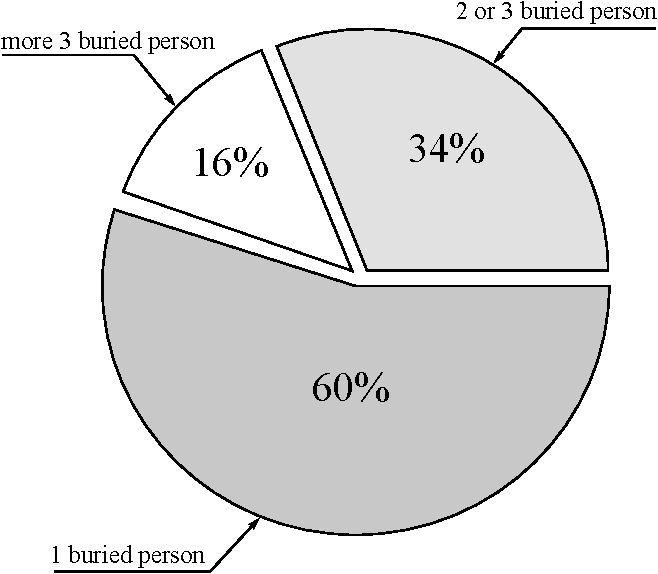
\includegraphics[width=5cm]{ch1/img/statistiche_sepolti.pdf}
	\caption{Number of buried}
\end{marginfigure}

Another important factor is the position of the overwhelms hikers:
\begin{itemize}
\item 37\% remain on the surface of the avalanche
\item 28\% are only partially buried
\item 35\% are completely buried
\end{itemize}

The survival curve, because of frostbite and hypothermia, without considerable traumas, has an upper limit of 15--18 minutes. Here is the the companion rescue that makes the real difference\cite{ManualeSciAlpinismo}.

One last important statistic is the number of hikers found with the ARTVA\marginnote{ARTVA: from the Italian \emph{Apparecchio Ricerca Travolti VAlanga}}. Considering the fact that the statistics do not take into account the episode of auto-rescue, the 7\% of the buried are found by the use of the receivers, a very small amount of the total. This data should be revised in the light of the advent of new digital ARTVA receivers, that simplify the searching method, and reduce the searching time \citep{hereforddigital}. 

As reported in \citep{Brugger2007}, within Europe and North America, avalanche airbags and avalanche transceiver reduce mortality, and companion rescue reduces incredibly the median duration of burial, remarking the extreme importance of those device for all mountaineers.

It is also known that 95\% of complete burial are in the layer between \num{-3} and\num{0} \si{\meter} of the avalanche.

\section{Avalanche Beacons}

There are two main typologies of avalanche transceiver. Differences are mostly in the user interface during receiving. We can divide in \emph{analog} and \emph{digital} ARTVA. Both device are equal for what concerns transmission. ARTVA can not be at the same time in transmission mode and receiving mode. Some models switch from receiving to transmission status after a scheduled amount of time. 

\subsection{Transmission Mode}

During transmission, beacons transmit a so-called \emph{wild-life tag}, or more simply, an intermittent signal at defined frequency, as stated in normative\cite{NormativaARVA}. From the normative, it is possible to extract more informations about the transmitted signal, that are listed in section \ref{sec:a1asegnale}.

\subsection{Receiving Mode}

The normative states for receiver:
\begin{itemize}
	\item the $(S+N)/N$ ratio of \num{6}\si{\decibel} at the terminal of electro--acoustic transducer
	\item a clear optical indication of direction for beacon with optical signal indication of direction
\end{itemize}
\marginnote{The Italian authority in Mountain Rescue is \emph{Soccorso Alpino e Speleologico Italiano}}

\myparagraph{Analog Beacons}
The analog beacon uses a cascade of filters and an identification circuit to extract the strength information of received signal. The strength is thus used as gain command for a sound generator, that rescuer uses to identify the direction of arrival. Typically, those ARTVA have a volume knob to perform a fine search. The main drawback is the extreme difficulty to perform a fast search, that requires an experienced user. Quoting \citep{457andfuture}: \emph{a better term for analog beacon would be \textbf{audible--based}}

\myparagraph{Digital Beacons}
Those beacons implements an user interface that indicates \emph{the field line direction and an artificial distance to the center of the field}. This simplicity makes those beacons perfect for unexperienced user and auto-rescue: those device \textbf{are strongly advised by the Mountain Rescue for all hikers, experienced or not}.

\begin{marginfigure}
	\centering
	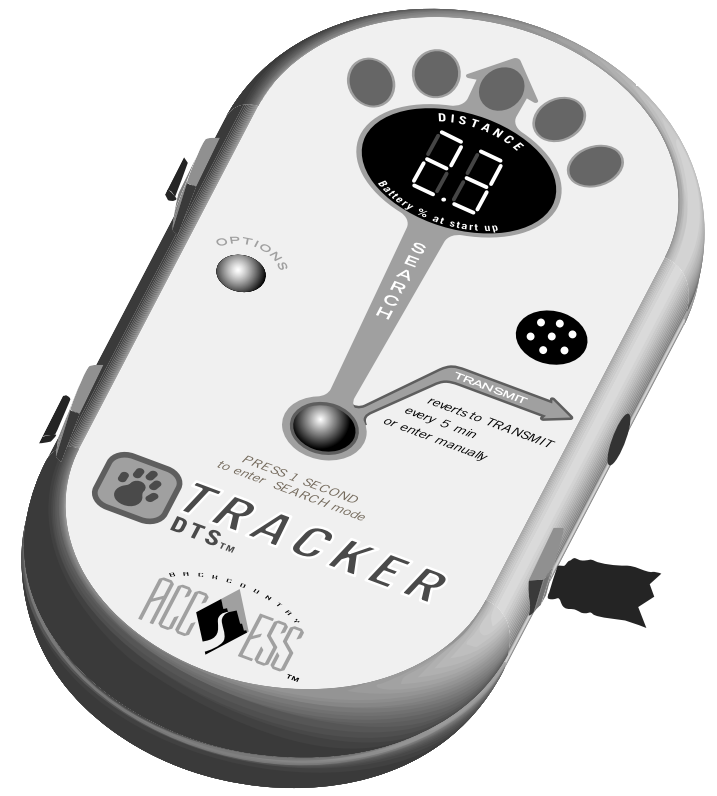
\includegraphics[width=4cm]{ch1/img/digital_baecon}
	\caption{Tracker DTS Avalanche Transceiver, a digital beacon}
\end{marginfigure}

Must be noted that the algorithm inside those transceivers runs on a very low power DPS, due to energy harvesting requirements, so often the rescuer must slow down his speed to gave time to the beacon to analyze received data. Also, it was pointed out from manufacturers that advanced techniques, like multi-buried identification and buried status (hearth-beat) make use of frequencies different from the one described in normative.

\subsection{Italian Mountain Rescue Intervention}
What happens after an avalanche? We interviewed some of the professionals of the Mountain Rescue Team in province of Trento, and asked them to explain us the actual procedure.

\myparagraph{Intervention on Avalanche}
The intervention begin after a witness call. Usually the witness is one of the hikers that is on the accident location. In the best situation, the witness begins the companion rescue procedure, with his own avalanche beacon, and calls the emergency number.

During the emergency call, the operator tries to understand the location, alerts the rescue team on shift and tries to figure out the general situation that the team may encounter. A rescue unit is formed by:
\begin{itemize}
\item Mountain Rescue heli-ambulance expert
\item Mountain Rescue canine unit
\item Health equip and nurse
\end{itemize}
If heli-ambulance is cleared to take off, those are the first rescuers on the avalanche. The clearance is related to weather and light conditions, because flight is performed by eye-sight. If heli-ambulance mission is aborted, Mountain Rescue team have to reach the avalanche with ground vehicle.

Under certain strict condition, it is possible to perform an ARTVA search from the helicopter.

Once arrived on the location, if residual risk make it possible, the rescue team is dropped from the heli-ambulance and starts the searching procedure, with canine unit and with personal ARTVAs. The rescuers with the beacons follow a scheme that allow them to cover the avalanche front. This scheme is called primary search. While a signal is identified, the rescuer start a fine search to pinpoint the buried position.

\myparagraph{Equipment}
There is a procedural and moral obligation in having the last generation device, even if does not exist a directive that defines a specific model for the equipment. Each rescuer has a VHF transmitter and cellphone, along with the personal beacon. 

It is possible to perform a search with other technology, like RECCO\sidenote[]{RECCO is a passive searching method, composed by a reflector included in hikers clothing, and a detector used by rescue teams. A RECCO detector usually performs passive search and \num{457}\si{\kilo\hertz} avalanche beacons search at the same time. The last generation detector has an average weight of \num{1}\si{\kilogram}, while the reflector weights only few grams. RECCO cannot be used for companion rescue}, even if the detector is heavy and not always reliable.

\section{State of the Art}

In this section we will analyze the state of the art in the field of beacons construction and signal analysis.

\subsection{Transmission}

Normative states the use of a very long wavelength ($\lunghezzaonda$) (\num{656}\si{\meter}). Such a long wavelength reduces the interference effects of snow, body and rocks and also multi-bouncing and multi-path effects\citep{balanis2012antenna} that may afflict some shorter waves. This is one of the main reason why GPS technology never erupted in this field\citep{457andfuture}.

This advantage also bring a consistent number of drawbacks, such as the fact that the search is always performed in near--field (distance less of $\lunghezzaonda/2\pi$). In the near--field, as we will see, interpretation of flux lines is quite complex, and it is difficult to derive a general direction of arrival algorithm.

Avalanche transceiver for companion rescue has to be small, therefore antennas and batteries has to be small. As we will see in the next chapter, to increase receiver antenna gain (also called effective height $\altezzaeffettiva$), ferrite core antennas are commonly used, but the efficiency and the noise introduced is not good. Those brings to transmitter that may be identified in the range of \numrange{40}{60}\si{\meter}, in function of type of receiver.

There is no big evolution in transmitters; almost all devices implement a simple amplitude--shifting--key (ASK) transmitter, build with an oscillator for the carrier, and a variable gain amplifier that modulates the intelligence signal.

\subsection{Reception}

Usually, an analog receiver has a little more bigger receiving radius with respect to a digital one. This difference is due to stronger filtration routines implemented in digital ARTVA, with respect to analog, and because of the dimension of the z--axis antenna.

A digital ARTVA implements multiple antennas. Some typical configurations are:
\begin{itemize}
\item two crossing antennas
\item three perpendicular antennas
\end{itemize}
The signal from whips are preprocessed using analog circuitry and then converted and processed in a DSP microprocessor. There are some advanced techniques\citep{Salos2007} implemented for the identification of the direction of the vectorial H--field, and also to help hikers and rescuers to find a transmitter. 

In general, the circuit may be resumed as follows:

\begin{figure}
	\centering
	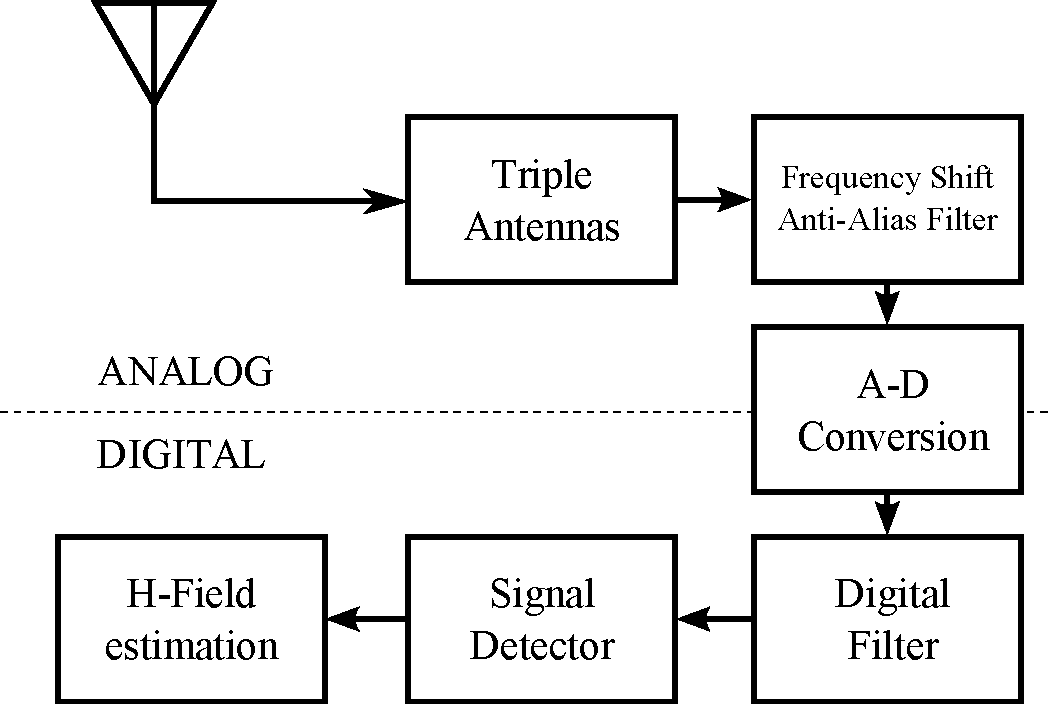
\includegraphics[width=7cm]{ch1/img/img_schema_arva.pdf}
	\caption{Block diagram of a commercial digital beacon, taken from \citep{Salos2007}}
	%\forceversofloat
\end{figure}


\begin{itemize}
\item signal is received through the antennas
\item the first stage of filtering is a frequency shift and  an anti-aliasing filter, that is necessary to avoid problems during AD-conversion
\item the signal is converted in the digital domain
\item other filtration techniques are analyzed  in \citep{Salos2007}, and are one of the main research topic in this field, in association with phase analysis to better understand the direction of the single components of the H--field
\item the signal detector and magnetic field estimator is implemented via software
\end{itemize}

One of the main challenge is the problem of the noise introduced by antennas. This noise is proportional to the received signal, phenomenon that induces an unsurmountable issue in the identification of multiple burial signal.

\subsection{Searching Algorithms}

\myparagraph{The magnetic momentum problem}
The main problem is the searching of the burial. Until now, only few are the example of automatic searching, while quite consolidated is the practice of the manual searching. One of the key aspects is the problem of the orientation of the transmitter: as we will see in the next chapter, the direction of the transmitter antenna change radically the shape of the field. From a general point of view, with respect to classical far--field identification problem, in this case we have to identify 6 state for each transmitter\sidenote[]{3 states refer to the position of the transmitter, while the latter 3 refers to the magnetic dipole momentum that is parallel to the axis of the antenna}, instead of 3, while we can only collect 3 measurements (the H--field vector components).

Even if there are some solutions for near--field qualitative direction of arrival, as explained in detail in \citep{hutchinson2000arrl}, typically those algorithms require a very prohibitive electro--mechanical circuitry, not suitable as mountain equipment (or in our case, a drone).

So far, only one solution earns the right to be cited: the solution proposed in \citep{pinies2006fast,pinies2006localization}, based upon Bayesian estimation theory and Kalman filters, is a remarkable attempt to find new approach to this problem, even if based on the weak assumption of a perfect knowledge of the covariance matrix related to the noise. One step ahead in this direction should be the redefinition of the problem in a dual form, from the Kalman filter to the information filter, in which the complete uncertainty is presented with a null matrix of the canonical form, instead of a infinite--valued matrix of the normal form. 

\myparagraph{Multiple Burial}
Those algorithms do not analyze the problem of multiple burial, and the subsequent possible situation of overlapping signal. An almost complete dissertation about this problem, with some test on beacon present on the market, may be found in \citep{signaloverlappingARVA1,signaloverlappingARVA2}. From those technical documents, distributed by one of the most well-know company in snow--safety, rises the evident lack of a solution for the overlapping problem, due to transmitted signal limitation. The most suggest solution is to run--away from an identified source in the hope to find another new signal. Some producer try to avoid this using parallel carrier frequency with additional information coded into intelligence signal (unique ID, heartbeat status, \dots). Those alternative frequencies are device/model dependent.

\myparagraph{A complex procedure}
Standard de facto is an algorithm of flux line following, in parallel with different assumption that user shall analyze, to derive the possible orientation of the buried person transmitting antenna, and subsequently find the best way to reach the hikers position. The complete explanation for the searching procedure is long even if not too complex, but based upon qualitative observation and deduction derived from expertise of the rescuer.

Generally speaking, what we need to know is the fact that a simple translation of this procedure in a machine with limited computational power is not practically possible.

A comprehensive description of the companion search and Mountain Rescue procedure could be found in \citep{ManualeSciAlpinismo}.

\section{Autonomous VTOL for buried searching}

The thesis is built around the main thread of inspect and derive the avionics of an autonomous VTOL. Even if avionics refer to the complete set of instrumentation and algorithms necessary to stabilize and control the flight, in this work we will focus on some of the main aspects necessary to perform the main task of buried searching.

This work is not the first attempt to bring an automatic drone on avalanches. Some remarkable examples are 
\begin{itemize}
\item SHERPA, European project born to create a robotic framework of helpers for Mountain Rescue, coordinated by University of Bologna
\item An user--piloted quad-copter research is just started in Politecnico di Torino
\item the project Alcedo from the Eidgen\"{o}ssische Technische Hochschule Z\"{u}rich\cite{projectAlcedoZurigo}
\end{itemize}

\subsection{Why the use of a VTOL?}
The use of a drone in the searching area depends on various factors. During design it is necessary to understand and think a system the fit entirely the actual search strategy.

One practical example of use could be a situation of high residual danger and an uncertainty about the presence of buried under the avalanche. In a case like that, the VTOL could be used to test the necessity of drop the rescue team on the avalanche.

The main advantage is obviously the ability to move faster on the avalanche with respect to an human rescuer, avoiding ground difficulties. At the same time, the drone should be able to identify and avoid obstacle like trees and ski--lift pillars.

\subsection{Quality Function Deployment}
The best way to define the characteristics of a new product is to inspect customer needs, and from qualitative user domain extrapolate quantitative engineering dimensions\cite{akao1994development}.

\myparagraph{Customer Needs}
From our interviews of Mountain Rescue members, we have derived some conclusions:
\begin{itemize}
\item one of the main cause of an avalanche is the weather, that modifies snow characteristics; during one day multiple avalanches may fall, so it is fundamental to guarantee a long, even if discontinue, operative time
\item the VTOL should be portable, with limited size and weight, but at the same time ready to be used in a short amount of time
\item all design process should take in to account the extreme low temperature and the high altitude (lower air density)
\item ARTVA device on the drone has to be robust with respect to electromagnetic interferences (propeller engines, radio, \dots)
\item user interface is simple while complete
\item the marking of the victims shall be hardware, with the use of visible darts
\end{itemize}
\begin{margintable}
	\begin{center}
		\begin{tabular}{ p{3.7cm} p{0.7cm} }
			\hline \textbf{Customer Need} & \textbf{Rating} \\ \hline
			Identifies buried person & 5 \\
			Is autonomous & 5 \\
			Returns to rescuer position & 5 \\
			Searches for the signall & 5 \\
			Is fast & 5 \\
			Marks physically buried position & 5 \\
			Operates at avalanche temperatures & 5 \\
			Performs more than one operation during the day & 3 \\
			Is usable by anyone & 3 \\
			Is robust with respect to EM interferences & 5 \\
			Is portable in a \num{35}\si{\liter} bag & 3 \\
			Is quiet & 2 \\
			Is compatible with other rescue vehicles & 5 \\
			Disengages from the winch & 5 \\
			Respects ENAC normatives & 3 \\
			\hline
		\end{tabular}
	\end{center}
	\caption{Customer needs \label{tbl:customer_needs}}
\end{margintable}

We are now able to define a table \ref{tbl:customer_needs} in which at each customer needs a rating is given.

In future, the automatic recognition of the avalanche dimensions could be a good starting point for some advanced research in the field of computer vision, or the improvements of user interface using voice recognition over radio.

\myparagraph{Technical Specification}
The next step in the definition of a good design is a list of technical specifications that will help us to identify the most challenging problems in and the gravity of those problems with respect to the costumer needs.

For sure, one of the first and most challenging complication is the weight reduction, that guarantees a longer flying time. Also those elements are related to the number of  propulsion vector and the main dimension (the length of the arm). It is evident the correlation between the number of lift vectors with respect to the maximum wind interference.

For the definition of a good searching algorithm, as we will see, it is important a good resolution of position and attitude of the drone; while to avoid obstacle it is important the resolution and the maximum revealing distance of the range finders.

One final aspect that should be considered are the data related to the system that performs the marking of a buried person.

All the specifications are listed in table \ref{tbl:tech_specs}
\begin{margintable}
	\begin{center}
		\begin{tabular}{ p{3.7cm}  p{0.7cm} }
			\hline \textbf{Technical Spec.} & \textbf{Dim.}  \\ \hline
			Flying time & \si{\minute} \\
			Weight & \si{\kilogram} \\
			N. of antennas & ~ \\
			Battery Temperature & \si{\celsius} \\
			Range Ultrasonic RF & \si{\meter} \\
			Arm Length & \si{\meter} \\
			Control TX distance & \si{\meter} \\
			GPS Resolution & \si{\meter} \\
			Lateral Speed & \si{\meter\per\second} \\
			 Wind Speed & \si{\meter\per\second} \\
			 ARTVA RX distance & \si{\meter} \\
			 Resolution Ultrasonic RF & \si{\meter} \\
			 Lift Force & \si{\newton} \\
			 N. dissembled pieces & ~ \\
			 N. Darts & ~ \\
			 N. Lift Vector & ~ \\
			 Maximum inclination & \si{\radian} \\
			 Operative height & \si{\meter} \\
			 IMU Resolution & \si{\meter\per\second} \\
			 Weight Marking Device & \si{\kilogram} \\
			 Weight Dart & \si{\kilogram} \\
			 Weight ARTVA & \si{\kilogram} \\
			\hline
		\end{tabular}
	\end{center}
	\caption{Technical specifications \label{tbl:tech_specs}}
\end{margintable}

% TODO invertire colonna 1 e 2 e nella nuoova colonna 2 inserire la dimensione 

\myparagraph{Merging the tables and comparison}
In table \ref{tbl:need_vs_spec} all data are compared with a weighting method. The table shows the comparison between technical specifications and customer needs and also between technical specifications and the other technical specifications.

\myparagraph{Components selection}
From the merged data it was possible to select the components that will be used in the prototype. All components are listed in table \ref{tbl:components_list}

We have also decide not to use a commercial ARTVA, but instead try to build a digital one from scratch. This will allow us to get a lighter model, and also extract exactly the information that we want from the received signal. Even if some device have a serial port, the output data are filtered with models that incorporate the possible speed of a rescue, that is different from our VTOL.
\begin{table}
	\begin{center}
		\begin{tabular}{ p{0.3cm} p{3.7cm} p{3.7cm} p{1cm} }
			\hline \scriptsize{\textbf{N}} & \footnotesize{\textbf{Component}} & \scriptsize{\textbf{Description}} & \footnotesize{\textbf{Price}} \\ \hline
			\scriptsize{$1\times$} & \footnotesize{Autoquad 6 Flight Controller} & \scriptsize{Imu board and stabilization controller} & \footnotesize{299.00\texteuro} \\
			\scriptsize{$6\times$} & \footnotesize{Autoquad ESC32} & \scriptsize{Electronic speed controller} & \footnotesize{239.40\texteuro} \\
			\scriptsize{$6\times$} & \footnotesize{Flyfuino HE4108 700kV Outrunner} & \scriptsize{Motors} & \footnotesize{299.40\texteuro} \\
			\scriptsize{$6\times$} & \footnotesize{HQ 12\inch per 4.5\inch CW and CCW Carbon propeller} & \scriptsize{Propeller} & \footnotesize{73.80\texteuro} \\
			\scriptsize{$2\times$} & \footnotesize{SLS Xtron \num{5000}\si{\milli\ampere\hour} \num{14.8}\si{\volt}} & \footnotesize{Batteries} & \footnotesize{119.98\texteuro} \\
			\scriptsize{$3\times$} & \footnotesize{USB UART Adapter} & \scriptsize{Bridge between USB and device UART} & \footnotesize{9.90\texteuro} \\
			\hline
			\multicolumn{3}{r}{\footnotesize{\textbf{Total}}}  & \footnotesize{1041.48\texteuro} \\
			\hline
		\end{tabular}
	\end{center}
	\caption{Components list \label{tbl:components_list}}
\end{table}

\newcommand{\rotatenovsmalll}[1]{\begin{sideways}\scriptsize{\textbf{#1}}\end{sideways}}
\newcommand{\smallbold}[1]{\scriptsize{\textbf{#1}}}

%\def\nine{\scriptsize{\textbf{9}}}
%\def\three{\scriptsize{3}}
\def\nine{\scriptsize{$\CIRCLE$}}
\def\three{\scriptsize{$\RIGHTcircle$}}
\def\point{\scriptsize{$\ocircle$}}

\def\upnin{\scriptsize{\begin{sideways}$\RHD$\end{sideways}}}
\def\upthr{\scriptsize{\begin{sideways}$\rhd$\end{sideways}}}
\def\dwnin{\scriptsize{\begin{sideways}$\LHD$\end{sideways}}}
\def\dwthr{\scriptsize{\begin{sideways}$\lhd$\end{sideways}}}

\begin{table*}[p]
    \centering
    \begin{tabular}{ b{4cm} b{0.08cm} b{0.08cm} b{0.08cm} b{0.08cm} b{0.08cm} b{0.08cm} b{0.08cm} b{0.08cm} b{0.08cm} b{0.08cm} b{0.08cm} b{0.08cm} b{0.08cm} b{0.08cm} b{0.08cm} b{0.08cm} b{0.08cm} b{0.08cm} b{0.08cm} b{0.08cm} b{0.08cm} b{0.08cm} }
    \hline
    \smallbold{Identifies buried person}                            &  \nine   &  \point  &  \nine   &  \point  &  \point  &  \point  &  \point  &  \nine   &  \three  &  \point  &  \nine   &  \point  &  \point  &  \point  &  \nine   &  \point  &  \point  &  \point  &  \point  &  \three  &  \three  &  \three  \\
    \smallbold{Is autonomous}                                       &  \three  &  \nine   &  \nine   &  \point  &  \nine   &  \point  &  \nine   &  \nine   &  \three  &  \nine   &  \nine   &  \three  &  \point  &  \point  &  \point  &  \point  &  \point  &  \point  &  \nine   &  \point  &  \point  &  \point  \\
    \smallbold{Returns to rescuers position}                        &  \nine   &  \point  &  \point  &  \point  &  \point  &  \point  &  \nine   &  \nine   &  \three  &  \nine   &  \point  &  \nine   &  \point  &  \point  &  \point  &  \point  &  \point  &  \three  &  \three  &  \point  &  \point  &  \point  \\
    \smallbold{Searches for the signal}                             &  \nine   &  \point  &  \nine   &  \point  &  \point  &  \point  &  \point  &  \nine   &  \nine   &  \point  &  \nine   &  \point  &  \point  &  \point  &  \point  &  \point  &  \point  &  \nine   &  \three  &  \point  &  \point  &  \nine   \\
    \smallbold{Is fast}                                             &  \three  &  \nine   &  \point  &  \point  &  \three  &  \nine   &  \point  &  \nine   &  \point  &  \nine   &  \point  &  \nine   &  \nine   &  \point  &  \point  &  \nine   &  \nine   &  \point  &  \nine   &  \three  &  \point  &  \point  \\
    \smallbold{Marks physically buried position}                    &  \point  &  \point  &  \point  &  \point  &  \point  &  \point  &  \nine   &  \nine   &  \point  &  \nine   &  \point  &  \nine   &  \point  &  \point  &  \nine   &  \point  &  \point  &  \point  &  \nine   &  \three  &  \nine   &  \point  \\
    \smallbold{Operates at avalanche temperature}                   &  \point  &  \point  &  \point  &  \nine   &  \point  &  \point  &  \nine   &  \nine   &  \point  &  \nine   &  \point  &  \nine   &  \point  &  \point  &  \point  &  \point  &  \point  &  \nine   &  \nine   &  \nine   &  \point  &  \point  \\
    \smallbold{Performs more than one operation during the day}     &  \nine   &  \three  &  \point  &  \nine   &  \point  &  \point  &  \point  &  \point  &  \point  &  \point  &  \point  &  \point  &  \three  &  \point  &  \three  &  \three  &  \point  &  \three  &  \point  &  \point  &  \three  &  \point  \\
    \smallbold{Is usable by anyone}                                 &  \point  &  \point  &  \point  &  \point  &  \three  &  \point  &  \three  &  \point  &  \point  &  \point  &  \point  &  \point  &  \point  &  \nine   &  \point  &  \point  &  \point  &  \point  &  \point  &  \three  &  \point  &  \point  \\
    \smallbold{Is robust with respect to EM}                        &  \point  &  \point  &  \nine   &  \point  &  \point  &  \point  &  \nine   &  \nine   &  \point  &  \nine   &  \three  &  \point  &  \point  &  \point  &  \point  &  \nine   &  \point  &  \point  &  \nine   &  \point  &  \point  &  \nine   \\
    \smallbold{Is portable  in a 35L bag}                           &  \point  &  \nine   &  \point  &  \three  &  \point  &  \nine   &  \point  &  \point  &  \point  &  \point  &  \point  &  \point  &  \point  &  \nine   &  \nine   &  \nine   &  \point  &  \point  &  \point  &  \point  &  \three  &  \nine   \\
    \smallbold{Is quiet}                                            &  \point  &  \point  &  \point  &  \point  &  \point  &  \point  &  \point  &  \point  &  \three  &  \point  &  \point  &  \point  &  \three  &  \point  &  \point  &  \nine   &  \three  &  \point  &  \point  &  \nine   &  \point  &  \point  \\
    \smallbold{Is compatible with other rescue vehicles}            &  \point  &  \point  &  \nine   &  \nine   &  \point  &  \point  &  \point  &  \nine   &  \point  &  \point  &  \nine   &  \point  &  \point  &  \point  &  \point  &  \point  &  \point  &  \point  &  \point  &  \point  &  \point  &  \point  \\
    \smallbold{Disengages from the winch}                           &  \point  &  \three  &  \point  &  \three  &  \point  &  \three  &  \point  &  \point  &  \point  &  \point  &  \point  &  \point  &  \point  &  \point  &  \point  &  \point  &  \point  &  \point  &  \point  &  \point  &  \nine   &  \nine   \\
    \smallbold{Respects ENAC normatives}                            &  \point  &  \nine   &  \three  &  \nine   &  \nine   &  \nine   &  \nine   &  \three  &  \three  &  \three  &  \point  &  \nine   &  \point  &  \point  &  \point  &  \nine   &  \point  &  \nine   &  \point  &  \three  &  \three  &  \three  \\
    \hline \\ 


    \scriptsize{\textbf{Legend}: \newline \scriptsize{\emph{Cust. needs vs. Tech. spec.}: \newline\point \hspace{1.5mm} no relation \newline\three \hspace{1.5mm} light relation \newline\nine \hspace{1.5mm} strong relation \newline \emph{Tech. spec. vs. Tech. spec.}: \newline\dwnin \hspace{1.5mm} negative strong relation \newline\dwthr \hspace{1.5mm} negative light relation \newline\point \hspace{1.5mm} no relation \newline\upthr \hspace{1.5mm} positive light relation \newline\upnin \hspace{1.5mm} positive strong relation}}

     & \rotatenovsmalll{Flying time} & \rotatenovsmalll{Weight} & \rotatenovsmalll{N. ARTVA antennas} & \rotatenovsmalll{Battery Temperature} & \rotatenovsmalll{Range Ultrasonic RF} & \rotatenovsmalll{Arm Length} & \rotatenovsmalll{Control TX distance} & \rotatenovsmalll{GPS resolution} & \rotatenovsmalll{Lateral speed} & \rotatenovsmalll{Wind speed} & \rotatenovsmalll{ARTVA RX distance} & \rotatenovsmalll{Resolution Ultrasonic RF} & \rotatenovsmalll{Lift Force} & \rotatenovsmalll{N. dissembled pieces} & \rotatenovsmalll{N. Darts} & \rotatenovsmalll{N. Lift vector} & \rotatenovsmalll{Maximum inclination} & \rotatenovsmalll{Operative Height} & \rotatenovsmalll{IMU resolution} & \rotatenovsmalll{Weight Marking Device} & \rotatenovsmalll{Weight Darts} & \rotatenovsmalll{Weight ARTVA}  \\
    \hline
    \multicolumn{2}{r}{\smallbold{Flying Time}}                                &  \dwnin  &  \dwthr  &  \dwthr  &  \point  &  \dwnin  &  \upthr  &  \upthr  &  \dwthr  &  \dwthr  &  \point  &  \point  &  \dwthr  &  \dwthr  &  \dwthr  &  \point  &  \point  &  \dwthr  &  \point  &  \dwnin  &  \dwnin  &  \dwnin  \\
    \multicolumn{3}{r}{\smallbold{Weight}}                                                &  \upnin  &  \upthr  &  \point  &  \upthr  &  \point  &  \point  &  \point  &  \upthr  &  \point  &  \point  &  \upthr  &  \upnin  &  \upnin  &  \upnin  &  \point  &  \point  &  \point  &  \upnin  &  \upnin  &  \upnin  \\
    \multicolumn{4}{r}{\smallbold{N. ARTVA antennas}}                                                &  \point  &  \point  &  \point  &  \point  &  \point  &  \point  &  \point  &  \upnin  &  \point  &  \dwthr  &  \upnin  &  \point  &  \point  &  \point  &  \point  &  \point  &  \point  &  \point  &  \upnin  \\
    \multicolumn{5}{r}{\smallbold{Battery temperature}}                                                         &  \point  &  \point  &  \point  &  \point  &  \dwthr  &  \point  &  \point  &  \point  &  \dwnin  &  \point  &  \point  &  \point  &  \point  &  \upnin  &  \point  &  \point  &  \point  &  \point  \\
    \multicolumn{6}{r}{\smallbold{Range Ultrasonic RF}}                                                                    &  \point  &  \point  &  \point  &  \upthr  &  \upthr  &  \point  &  \dwnin  &  \point  &  \point  &  \point  &  \point  &  \upnin  &  \point  &  \point  &  \point  &  \point  &  \point  \\
    \multicolumn{7}{r}{\smallbold{Arm length}}                                                                                        &  \point  &  \point  &  \upnin  &  \upnin  &  \point  &  \point  &  \dwthr  &  \point  &  \point  &  \point  &  \upthr  &  \point  &  \point  &  \point  &  \point  &  \point  \\
    \multicolumn{8}{r}{\smallbold{Control TX distance}}                                                                                          &  \upthr  &  \upthr  &  \point  &  \point  &  \point  &  \point  &  \point  &  \point  &  \point  &  \point  &  \point  &  \point  &  \point  &  \point  &  \point  \\
    \multicolumn{9}{r}{\smallbold{GPS Resolution}}                                                                                                          &  \point  &  \upthr  &  \point  &  \point  &  \point  &  \point  &  \point  &  \point  &  \point  &  \point  &  \dwthr  &  \point  &  \point  &  \point  \\
    \multicolumn{10}{r}{\smallbold{Lateral speed}}                                                                                                                     &  \point  &  \point  &  \point  &  \upnin  &  \point  &  \point  &  \upnin  &  \upnin  &  \point  &  \point  &  \point  &  \point  &  \point  \\
    \multicolumn{11}{r}{\smallbold{Wind speed}}                                                                                                                                   &  \point  &  \point  &  \upnin  &  \point  &  \point  &  \upnin  &  \upthr  &  \point  &  \upnin  &  \upthr  &  \upthr  &  \upthr  \\
    \multicolumn{12}{r}{\smallbold{ARTVA RX distance}}                                                                                                                                       &  \point  &  \point  &  \point  &  \point  &  \point  &  \point  &  \point  &  \point  &  \point  &  \point  &  \upnin  \\
    \multicolumn{13}{r}{\smallbold{Resolution Ultrasonic RF}}                                                                                                                                           &  \point  &  \point  &  \point  &  \point  &  \point  &  \point  &  \point  &  \point  &  \point  &  \point  \\
    \multicolumn{14}{r}{\smallbold{Lift Force}}                                                                                                                                                                    &  \point  &  \point  &  \upnin  &  \upthr  &  \upnin  &  \point  &  \point  &  \point  &  \point  \\
    \multicolumn{15}{r}{\smallbold{N. disassembled pieces}}                                                                                                                                                                   &  \upnin  &  \upnin  &  \point  &  \point  &  \point  &  \upthr  &  \upthr  &  \upthr  \\
    \multicolumn{16}{r}{\smallbold{N. Darts}}                                                                                                                                                                                            &  \point  &  \point  &  \point  &  \point  &  \upnin  &  \dwnin  &  \point  \\
    \multicolumn{17}{r}{\smallbold{N. Lift vector}}                                                                                                                                                                                                 &  \upnin  &  \upnin  &  \point  &  \point  &  \point  &  \point  \\
    \multicolumn{18}{r}{\smallbold{Maximum inclination}}                                                                                                                                                                                                       &  \dwthr  &  \point  &  \point  &  \point  &  \point  \\
    \multicolumn{19}{r}{\smallbold{Operative Height}}                                                                                                                                                                                                                     &  \point  &  \point  &  \point  &  \point  \\
    \multicolumn{20}{r}{\smallbold{IMU Resolution}}                                                                                                                                                                                                                                  &  \point  &  \point  &  \point  \\
    \multicolumn{21}{r}{\smallbold{Weight Marking Device}}                                                                                                                                                                                                                                      &  \upnin  &  \point  \\
    \multicolumn{22}{r}{\smallbold{Weight Darts}}                                                                                                                                                                                                                                                          &  \point  \\
    \end{tabular}
    \caption{Comparison Table\label{tbl:need_vs_spec}}
    \forceversofloat
\end{table*}

%\marginnote{\textbf{How to read table \ref{tbl:need_vs_spec}}: \newline \scriptsize{\emph{Cust. needs vs. Tech. spec.}: \newline\point \hspace{1.5mm} no relation \newline\three \hspace{1.5mm} light relation \newline\nine \hspace{1.5mm} strong relation \newline \emph{Tech. spec. vs. Tech. spec.}: \newline\dwnin \hspace{1.5mm} negative strong relation \newline\dwthr \hspace{1.5mm} negative light relation \newline\point \hspace{1.5mm} no relation \newline\upthr \hspace{1.5mm} positive light relation \newline\upnin \hspace{1.5mm} positive strong relation}}

\let\nine\undefined
\let\three\undefined
\let\point\undefined
\let\upnin\undefined
\let\upthr\undefined
\let\dwthr\undefined
\let\dwnin\undefined

\FloatBarrier

	% CHAPTER 2

\chapter{Design of a digital ARTVA \label{ch:chapter2}}
\minitoc
%% Enlarge array size
\renewcommand{\arraystretch}{2}

In this chapter we will try to design a digital receiver for the ARTVA signal. Before starting with the design, \emph{ARTVA signal} is deeply analyzed, with the derivation of a simplified model for a field pattern that could be used  for the implementation of the searching algorithm. After that, ferrite antennas are studied, as they are the only way to receive such a long wavelength. In the last part of the chapter the circuitry for the ARTVA receiver is shown and explained.

\section{Analysis of transmitting pattern}

A formal model of the transmitting pattern is fundamental for the implementation of the searching algorithm. We start from the basic Maxwell's equation and we arrive to a simpler model numerically usable.

As we will see, radiating pattern is quite complex due to the fact that we are working in the \textbf{near--field} region, condition that constraint us to not use classical DoA\marginnote{\emph{DoA}: Direction of Arrival}, such as MUSIC or ESPRIT, that operates in far-field condition and at higher frequencies. DoA systems for long waves usually requires too big electro--mechanical devices.

\subsection{Maxwell's Equations}
The following investigation is based upon Maxwell's Equation, in which the magnetic permeability $\magperm$ and dielectric constant $\dielettrico$ are considered constant (the radiation is assumed to propagate at speed of light in air). Also we consider some field properties, that are function of radio distance $\radiodist$ and time $t$:
\[
f(\radiodist,t) = f \qquad f \in \left[\; \chargedens,\; \currdens,\; \efield,\; \bfield,\; \hfield \; \right]
\]
The equations that rule the induction are the \emph{Gauss equation of magnetic induction} and the \emph{Faraday law of electric induction}:
\begin{equation}
\nabla\cdot\bfield = 0
\label{eq:gauss1}
\end{equation}
\begin{equation}
\nabla\times\efield = -\partialt \bfield
\label{eq:faraday}
\end{equation}
while the equations that rule the interaction with materials are \emph{Gauss equation} and \emph{Ampere law}:
\begin{equation}
\nabla\cdot\efield = \dfrac{\chargedens}{{\dielettrico}_0}
\label{eq:gauss2}
\end{equation}
\begin{equation}
\nabla\times\bfield = {\magperm}_0 \left( \currdens + {\dielettrico}_0 \partialt \efield \right)
\label{eq:ampere}
\end{equation}

\subsection{EM field dynamic potentials}

Starting from equation \ref{eq:gauss1}, we can define a vectorial function called \emph{potential vector} $\afield$ of $\bfield$:
\begin{equation}
\bfield = \nabla\times\afield
\label{eq:potvett}
\end{equation}
\marginnote{The existence of $\afield$ is verified by property of $\nabla$ operator, whom states that the divergence of a curl of a vector field is zero\citep{bramanti2009analisi}} 
We insert \ref{eq:potvett} in \ref{eq:faraday}:
\[
\nabla\times\efield = - \partialt \left( \nabla\times\afield \right)
\]
\begin{equation}
\nabla\times\left( \efield + \partialtarg{\afield} \right) = 0
\end{equation}
From the previous equation it is evident that the argument between parentheses is an irrotational vector field, thus a potential function exists such that:
\[
-\nabla\scpot = \efield + \partialtarg{\afield}
\]
and we derive the following definition of electric field:
\begin{equation}
\efield = - \nabla \scpot - \partialtarg{\afield}
\label{eq:efieldvett}
\end{equation}
Equation \ref{eq:potvett} and \ref{eq:efieldvett} are used to express a new formulation for the Maxwell's equation based upon vector potential\sidenote{The proof is in chapter appendix \ref{eq:evidence1}}:
\begin{equation}
\begin{array}{rcl}
\nabla^2\scpot + \partialt \nabla \cdot \afield & = & - \dfrac{\chargedens}{\dielettrico_0} \\
\nabla^2 \afield - \dfrac{1}{\velocitaluce^2} \partialttarg{\afield} - \nabla\left( \nabla \cdot \afield + \dfrac{1}{\velocitaluce^2} \partialtarg{\scpot} \right) & = & -\magperm_0 \currdens
\end{array}
\label{eq:potvecmaxwell}
\end{equation}
Those equation, even if complex, could be resolved with a well posed boundaries condition problem. Equation are coupled with the current formulation, but could be decoupled using the \textbf{Gauge transformation}\citep{mencuccini1988fisica}, also called \textbf{recalibration map}, that is in the form:
\begin{equation}
\left\{ \begin{array}{rcl}
\afield' & \mapsto & \afield + \nabla \lorentz \\
\scpot' & \mapsto & \scpot - \partialtarg{\lorentz}
\end{array}
\right.
\end{equation}
in which $\lorentz = \lorentz(\radiodist,t) \in C^2$. As proofed in \ref{eq:prooftransformationmap}, this map represents an invariant with respect to dynamic potential formulation. If we consider a $\lorentz$ such that it verifies the \textbf{Lorentz equation}
\begin{equation}
\nabla \cdot \afield' = - \dfrac{1}{\velocitaluce^2} \partialtarg{\scpot'}
\end{equation}
we obtain the decoupled version:
\begin{equation}
\begin{array}{rcl}
\nabla^2 \scpot - \dfrac{1}{\velocitaluce^2} \partialttarg{\scpot} & = & - \dfrac{\chargedens}{\dielettrico_0} \\
\nabla^2 \afield - \dfrac{1}{\velocitaluce^2} \partialttarg{\afield} & = & - \magperm_0 \currdens 
\end{array}
\end{equation}
Those dynamic equations describe the time evolution of an EM--field. If field sources are located in a finite region, the problem admit as solution a generalization of the well know stationary formulation, called retarded potential:
\begin{equation}
\begin{array}{rcl}
\scpot(\radiodist,t) & = & \dfrac{1}{4\pi \dielettrico_0} \displaystyle\iiint\limits_{\Omega} \dfrac{1}{\mid \radiodist - \radiodist' \mid} \chargedens\left( \radiodist',t-\dfrac{\mid \radiodist - \radiodist' \mid}{\velocitaluce} \right) d\radiodist   \\
\afield(\radiodist,t) & = & \dfrac{\magperm_0}{4\pi} \displaystyle\iiint\limits_{\Omega} \dfrac{1}{\mid \radiodist - \radiodist' \mid} \currdens\left( \radiodist',t-\dfrac{\mid \radiodist - \radiodist' \mid}{\velocitaluce} \right) d\radiodist 
\end{array}
\end{equation}
in which the vector distance ${\radiodist - \radiodist'}$ is the distance between the point where retarded potential is evaluated and the point where the element of volume $d\radiodist$ of the localized sources is located. The delay is due to the definition of time:
\[
t_r = t - \dfrac{\mid \radiodist - \radiodist' \mid}{c}
\]

\subsection{Magnetic dipole radiation}

\myparagraph{Potential of a magnetic dipole}
Our antenna may be seen as an ideal magnetic dipole\citep{balanis2012antenna}. The transmitting antenna is a solenoid with a ferrite core, that acts as source of the electro--magnetic field. The source is subject to a dipole magnetic moment induced by the current $J = J_0 \cos(\omegaarva t)$, with no free charges (null scalar potential). 
\begin{figure}[h]
	\centering
	
	\tdplotsetmaincoords{60}{130}
	\begin{tikzpicture}[auto,>=latex,tdplot_main_coords]
		\coordinate (origin) at (0,0,0);
		
		% Axis
		\draw [->] (origin) -- (4,0,0) node[anchor=north east]{\scriptsize{$x$}}; \draw (origin) -- (-0.2,0,0);
		\draw [->] (origin) -- (0,4,0) node[anchor=north west]{\scriptsize{$y$}}; \draw (origin) -- (0,-0.2,0);
		\draw [->] (origin) -- (0,0,2) node[anchor=south]{\scriptsize{$z$}}; \draw (origin) -- (0,0,-0.2);

		\tdplotdrawarc[->,line width=3]{(0,0,0)}{2.7}{90}{360+80}{}{}
		\tdplotdrawarc[line width=6]{(0,0,0)}{2.7}{25}{35}{}{}
		\tdplotdrawarc[<->]{(0,0,0)}{3.5}{0}{30}{anchor=north west,xshift=-10}{$\varphi'$}
		\coordinate (drpoint) at (30:2.7);
		\node at (-2.3,2.3,0) {$\mathbf{J}$};
		\node [at=(drpoint),xshift=5,yshift=-10] {$d\mathbf{r}$};

		\node [circle,draw,inner sep=1pt, fill=black] at (7.5,0,6) (rpoint) {};
		\draw[->] (origin) -- node[pos=0.8,above]{$\mathbf{r}$} (rpoint);
		\draw [dashed] (rpoint) -- (7.5,0,0) -- ++(-2.5,0,0);
		\coordinate [at=(drpoint),yshift=3] (drpoint2);
		\draw [<->] (rpoint) -- node[pos=0.425,below,xshift=-22]{$\kappa=|\mathbf{r}-\mathbf{r}'|$} (drpoint2);
		\draw [->] (origin) -- node[right]{$\mathbf{r}'$} (drpoint2);

		\tdplotsetrotatedcoords{90}{90}{180}
		\tdplotsetrotatedcoordsorigin{(origin)}
		\draw[tdplot_rotated_coords,<->] (0.5,0) arc (0:52.5:0.5) node[left,xshift=5,yshift=10]{$\theta$};

		\tdplotsetrotatedcoords{29.5+270}{-23.75}{0}
		\tdplotsetrotatedcoordsorigin{(origin)}
		\draw[tdplot_rotated_coords,<->] (0.75,0) arc (0:90:0.75) node[left,xshift=-15,yshift=10]{$\psi$};
		
	\end{tikzpicture}
	\tdplotsetmaincoords{0}{0}

	\caption{Formulation of magnetic dipole problem}
	\label{eq:dipolomagnetico}
	\forceversofloat
\end{figure}
The magnetic dipole moment is:
\begin{equation}
\magdipole = \pi r'^2\; J \vrz = m_0 \cos(\omegaarva t) \vrz
\label{eq:dipolodacorrente}
\end{equation}
From figure \ref{eq:dipolomagnetico} we define the retarded potential equation, with ${\kappa = \mid \radiodist-\radiodist'\mid}$:
\[
\afield(\radiodist,t) = \dfrac{\magperm_0}{4\pi}\int{\dfrac{J_0\cos(\omegaarva (t - \kappa/c))}{r}\ccos{\varphi'}d\varphi'}\hat{\boldsymbol{\phi}}
\]
In the hypothesis of ${\radiodist\parallel\vrz\times\vrx}$, we obtain a vector $\afield$ directed along $\vry$:
\[\begin{array}{rcl}
\radiodist & = & r \sin(\theta) \vrx + r \cos(\theta) \vrz \\
\radiodist' & = & r' \cos(\varphi') \vrx + r' \sin(\varphi') \vry \\
\kappa & = & \sqrt{(\radiodist - \radiodist')\cdot(\radiodist - \radiodist')}
\end{array}\]
Those elements in retarded potential formulation lead us to the integral formulation that has only one angular dependency:
\begin{equation}
\label{eq:integraledacalc}
\afield(\radiodist,t) = \dfrac{\magperm_0 J_0 r'}{4\pi}\int\limits_{0}^{2\pi}{\dfrac{\cos(\omegaarva (t - \kappa/c))}{\kappa} \cos(\varphi') d\varphi' \hat{\boldsymbol{\phi}}}
\end{equation}
The solution of this integral is reported in appendix; we recall only the simplification used:
\begin{itemize}
\item we assume $r' \ll r$
\item we assume $r' \ll \lambda = 2\pi c/\omegaarva$
\end{itemize}
that brings us to the following solution:
\begin{equation}
\label{eq:soluzioneint}
\afield(\radiodist,t) = \dfrac{\magperm_0 m_0}{4\pi r}\,\sin(\theta)\left( \dfrac{1}{r} \sin\left(\omegaarva(t-r/c)\right) - \dfrac{\omegaarva}{r}\cos\left(\omegaarva(t-r/c)\right)\right)\hat{\boldsymbol{\phi}}
\end{equation}
in which $m_0$ identifies the total dipole moment, considering also the number of the coils of antenna. The rest of the equation describes the propagation of the transmission in near--field conditions.

\myparagraph{Electric and magnetic field}
With null scalar potential we obtain the electric field and the magnetic field from the equations:
\begin{equation}
\begin{array}{rcl}
\efield & = & - \partialtarg{\afield} \\
\bfield & = & \nabla\times\afield 
\end{array}
\end{equation}
The application of differential operator $\nabla$:
\marginnote{In polar coordinates: \newline $\nabla=\left[ \begin{array}{c} \dfrac{\partial}{\partial r} \\ \dfrac{1}{r}\;\dfrac{\partial}{\partial\theta} \\ \dfrac{1}{r \sin(\theta)}\;\dfrac{\partial}{\partial\phi} \end{array} \right]$}
\begin{equation}
\efield = \left[ \begin{array}{c} 0 \\ 0 \\ \partialtarg{A_{\phi}} \end{array} \right]
\qquad
\bfield = \left[ \begin{array}{c} \dfrac{1}{r}\;\dfrac{\partial A_{\phi}}{\partial \theta} \\ - \dfrac{\partial A_{\phi}}{\partial r} \\ 0 \end{array} \right]
\end{equation}
The final formulation for th EM field of a magnetic dipole is\citep{knoepfel2008magnetic}:
\begin{equation}
\begin{array}{rcl}
\label{eq:campidef1}
\tau & = &  t - \dfrac{r}{\velocitaluce} \\
E_{\phi} & = & \dfrac{\magperm_0 m_0}{4\pi}\sin(\theta)\left( \dfrac{\omegaarva}{r^2}\sin\left( \omegaarva\tau \right) + \dfrac{\omegaarva^2}{c}\cos\left( \omegaarva\tau \right) \right) \\
B_{r} & = & \dfrac{\magperm_0 m_0}{2\pi r^2}\cos(\theta)\left( \dfrac{1}{r}\cos\left( \omegaarva\tau \right) + \dfrac{\omegaarva}{c}\sin\left( \omegaarva\tau \right) \right) \\
B_{\theta} & = & \dfrac{\magperm_0 m_0}{4 \pi r^3 c^2}\sin(\theta)\left( \left( \velocitaluce^2 - \omegaarva^2 r^2 \right)\cos\left( \omegaarva\tau \right) + \omegaarva r \velocitaluce \sin\left( \omegaarva\tau \right) \right) 
\end{array}
\end{equation}
In figure \ref{fig:animazionifield} are shown some animation referred to the magnetic field defined in the previous equations. The animation are performed using ARTVA typical parameters, even if time is scaled. The equations are parametric with respect to a value, $m_0$ that is the transmitter magnetic dipole. As we have seen in chapter \ref{ch:chapter1}, the real transmitting power of an avalanche beacon is not known, but it shall have the maximum at \num{10}\si{\meter} inside a range. The animations consider an unitary magnetic dipole moment.

\begin{figure*}[p]
\label{fig:animazionifield}
\animategraphics[width=6.5cm,autoplay,loop]{15}{ch2/img/xz_10m/animation_}{0}{59}
\animategraphics[width=6.5cm,autoplay,loop]{15}{ch2/img/xz_40m/animation_}{0}{59} \newline
\animategraphics[width=6.5cm,autoplay,loop]{15}{ch2/img/xz_100m/animation_}{0}{59}
\animategraphics[width=6.5cm,autoplay,loop]{15}{ch2/img/xz_2lambda/animation_}{0}{59} \newline
\animategraphics[width=6.5cm,autoplay,loop]{15}{ch2/img/xy_10m/animation_}{0}{59} 
\animategraphics[width=6.5cm,autoplay,loop]{15}{ch2/img/xy_2lambda/animation_}{0}{59}
\caption{Graphical animation of the magnetic field $\bfield$ with retarded potential formulation. Those graph derives directly from the equations \ref{eq:campidef1}. To see the animations, please use \texttt{Adobe Acrobat viewer}}
\end{figure*}

\subsection{Magnetic field model simplification}
From animations it is evident that the effect of retarded propagation is almost null inside a radius of \num{40}\si{\meter} from the transmitting source, that is roughly the maximum distance at which an avalanche beacon receives the signal. This brings us to other simplifications for our model, as we will see in this section. From now on, all the simplifications are performed with the intent to find a model computationally convenient to be used in our algorithms.

\myparagraph{Re--definition in complex domain}
The next step is to bring equation of magnetic field in complex domain, but keeping in mind that only real part of the equations retains the physical meaning of the field. The re--interpretation is based upon Euler relationship and on the definition of wavenumber:
\[
e^{j\beta} = \ccos{\beta} + j \ssin{\beta}
\]
\[
\numeroonda = \dfrac{\omegaarva}{\velocitaluce}
\]
\begin{equation}
\begin{array}{rcl}
B_r & = & \dfrac{1}{2} \dfrac{\magperm_0 m_0}{\pi} \ccos{\theta} \braces{\dfrac{1}{r^3}\ccos{\omegaarva \tau} - \dfrac{\kappa}{r^2} \ssin{\omegaarva \tau}} \\
 & = & -\dfrac{1}{2} j \dfrac{\magperm_0 m_0}{\pi} \kappa^3 \ccos{\theta} \braces{\dfrac{1}{j^2 r^2 \kappa^2} + \dfrac{1}{j^3 r^3 \kappa^3}} e^{j\omegaarva \tau}
\end{array}
\end{equation}
\begin{equation}
\begin{array}{rcl}
B_{\theta} & = & \dfrac{1}{4} \dfrac{\magperm_0 m_0}{\pi r^3 c^2} \ssin{\theta} \braces{\braces{\velocitaluce^2 - \omegaarva^2 r^2}\ccos{\omegaarva \tau} - \omegaarva r \velocitaluce \ssin{\omegaarva \tau}} \\
 & = & -\dfrac{1}{4} j \dfrac{\magperm_0 m_0}{\pi} \kappa^3 \ssin{\theta} \braces{\dfrac{1}{j r \kappa} + \dfrac{1}{j^2 r^2 \kappa^2} + \dfrac{1}{j^3 r^3 \kappa^3}} e^{j\omegaarva \tau}
\end{array}
\end{equation}
The proof of those relations is in appendix.

\myparagraph{From Polar to Cartesian coordinates}
\begin{marginfigure}
	\centering
	%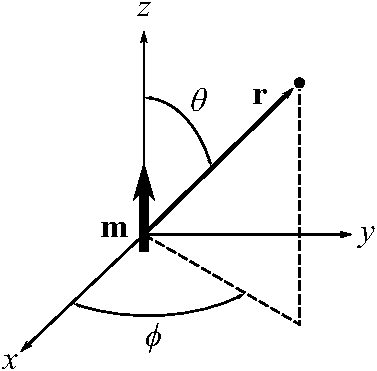
\includegraphics[width=4cm]{ch2/img/coord_pol_cart.pdf}
	\tdplotsetmaincoords{70}{110}
	\begin{tikzpicture}[auto,>=latex,tdplot_main_coords]
		\coordinate (origin) at (0,0,0);
		\tdplotsetrotatedcoords{-45}{-90}{0}
		\tdplotsetrotatedcoordsorigin{(origin)}
		%\riferimento
		% Axis
		\draw [->] (origin) -- (3,0,0) node[anchor=north east]{\scriptsize{$x$}}; \draw (origin) -- (-0.2,0,0);
		\draw [->] (origin) -- (0,2.5,0) node[anchor=west]{\scriptsize{$y$}}; \draw (origin) -- (0,-0.2,0);
		\draw [->] (origin) -- (0,0,2.5) node[anchor=south]{\scriptsize{$z$}}; \draw (origin) -- (0,0,-0.2);

		\draw[->,line width=2] (0,0,-0.1) -- node[left]{$\hat{\mathbf{m}}$} (0,0,1.5);
		\node [circle,draw,inner sep=1pt, fill=black] at (3,3,3) (rpoint) {};
		\draw [->] (origin) -- node[pos=0.8,above]{$\mathbf{r}$} (rpoint);
		\draw [dashed] (origin) -- (3,3,0) -- (3,3,3);
		\draw[tdplot_rotated_coords,<->] (2,0) arc (0:55:2) node[pos=0.5]{$\theta$};
		\draw [<->] (2,0,0) arc (0:45:2) node[pos=0.5,below]{$\phi$};
	\end{tikzpicture}
	\caption{From Polar coordinates to Cartesian coordinates}
	\label{fig:polar2cartesian}
\end{marginfigure}
\begin{marginfigure}
	\centering
	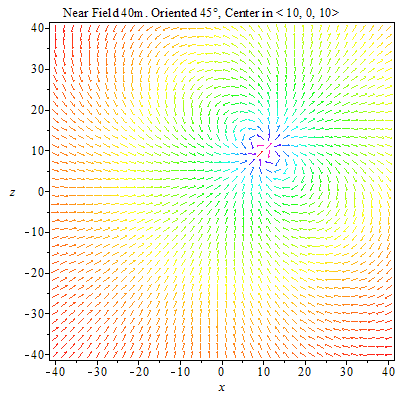
\includegraphics[width=5cm]{ch2/img/campo_casuale.png}
	\caption{Representation of a magnetic field with source: \newline $\postx = [10, 0, 10]^T$ \newline $\magdipole=[\ccos{\pi/4},0,\ssin{\pi/4}]^T$}
	\label{fig:dipolomagneticocasuale}
\end{marginfigure}
The last approximation is related to the nature of the receiver:
\begin{itemize}
\item the receiver act as an identifier of the constant quantity of the field, or the magnitude of the oscillating field
\item the distance of the receiver is always in a radius that allows us to not consider the effect of retarded potential: 
		\[\tau = \left. t - \dfrac{r}{c} \;\right|_{r\ll c}  \longrightarrow t \]
\end{itemize}

Under those considerations, and with MacLaurin first order transformation of $B_{\theta}$, the formulation of magnetic field real part takes the form:
\begin{equation}
\bfield = \dfrac{\magperm_0}{4 \pi r^3} \braces{ 2 m_0 \ccos{\theta} \vers{r} + m_0 \ssin{\theta} \vrtheta }
\label{eq:magneticfieldpolar}
\end{equation}

The projection of the field in cartesian coordinates is:
\begin{equation}
\bfield(\radiodist,\magdipole) = \dfrac{\magperm_0}{4 \pi r^5} \magfieldmatrix \magdipole
\end{equation}
A final generalization grants us the ability to write a general form of the field that has origin in position different from the origin:
\begin{equation}
\bfield(\hexastate - \postx,\magdipole)
\end{equation}
That is the form used for our simulations.

\section{Analytical signal analysis - A1--A \label{sec:a1asegnale}}

The ARTVA signal is a wild-life tag, specifically an \textbf{A--1A} signal. From the normative\cite{NormativaARVA}:
\begin{itemize}
\item A1A Signal:
	\begin{itemize}
	\item amplitude modulated signal
	\item digital information (keying)
	\item carrier frequency: \num{457}\si{\kilo\hertz}
	\item no auxiliary carrier
	\item frequency error shall not exceed $\pm$\num{80}\si{\hertz}
	\end{itemize}
\item carrier keying characteristics:
	\begin{itemize}
	\item on-time: \num{70}\si{\milli\second} minimum
	\item off-time: \num{400}\si{\milli\second} minimum
	\item period: \num{1000}\si{\milli\second} $\pm$ \num{300}\si{\milli\second}
	\end{itemize}
\item H--field peak at \num{10}\si{\meter}
	\begin{itemize}
	\item must be greater than \num{0.5}\si{\micro\ampere\per\meter}
	\item must be lower than \num{2.23}\si{\micro\ampere\per\meter}
	\end{itemize}
\end{itemize}

\begin{marginfigure}
	\centering
	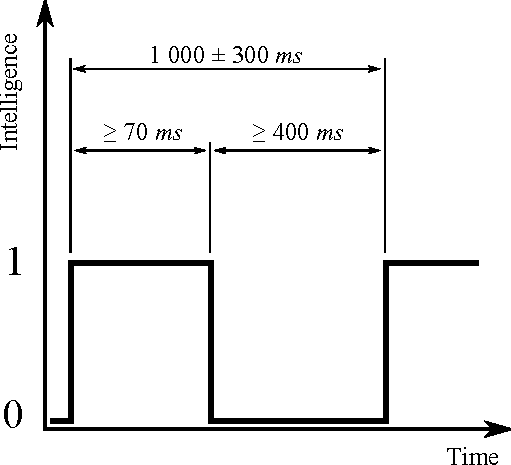
\includegraphics[width=5cm]{ch1/img/artva_signal.pdf}
	\caption{Intelligence signal of avalanche beacons}
	\label{fig:squarewaves}
\end{marginfigure}

The variable duty cycle is a challenge for the formulation of a searching algorithm, with a duty cycle ($\dutycycle$) that varies from a minimum of 5.4\% to a maximum of 42.9\%. The amplitude modulation, from a mathematical point of view is:
\begin{equation}
\jtx(t) = \braces{1+\mu \,\jint}\ccos{\omegaarva t}
\end{equation}
\begin{marginfigure}
	\centering
	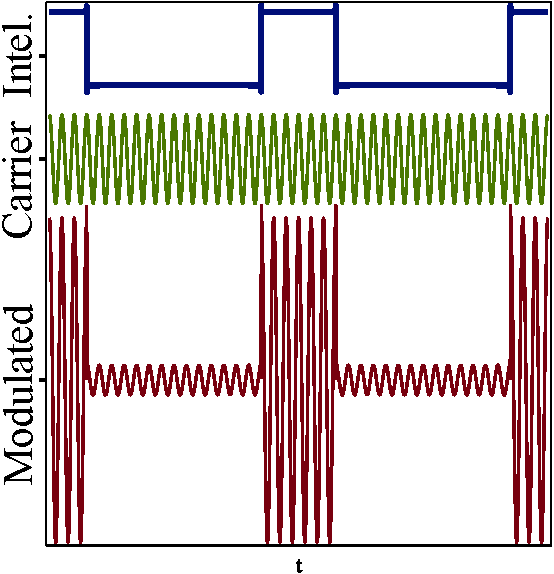
\includegraphics[width=5cm]{ch2/img/modulation_example.pdf}
	%\forceversofloat
	\caption{Example of a A--1A modulated signal}
	%\forceversofloat
\end{marginfigure}
There are 3 key elements:
\begin{itemize}
\item $\jint$ is the current of the intelligence signal, the representation of the square wave in figure \ref{fig:squarewaves}:
\begin{equation}
\jint(t) = A\dutycycle + \sum\limits_{n=1}^{\infty}\braces{\dfrac{2A}{n\pi}\ssin{n\pi \dutycycle} \ccos{\omegaint n t}}
\end{equation}
in which $A$ represents the signal amplitude and $\Delta$ is the duty cycle. 
\item the frequency of the carrier signal is ${f_0 = 2\pi\omegaarva}$, and it is \num{457}\si{\kilo\hertz}
\item $\mu$ is called modulation factor
\end{itemize}
From this current we are able to obtain the magnitude of dipole magnetic vector, using equation \ref{eq:dipolodacorrente}. Many of those parameter are device dependent and not known.

\section{Receiving antenna}

To receive such a long wavelenght for our appplication there is almost only one solution: use a ferrite core loop antenna, that is also the antenna used for transmission. In the next section, ferrite antenna is analyzed deeply, as a crucial part for the receiver. As we will see from the prototype, obtain a good receiver antenna is a very difficult task.

\subsection{Coils receiver}

\myparagraph{Single coil receiver}
\begin{marginfigure}
	\centering
	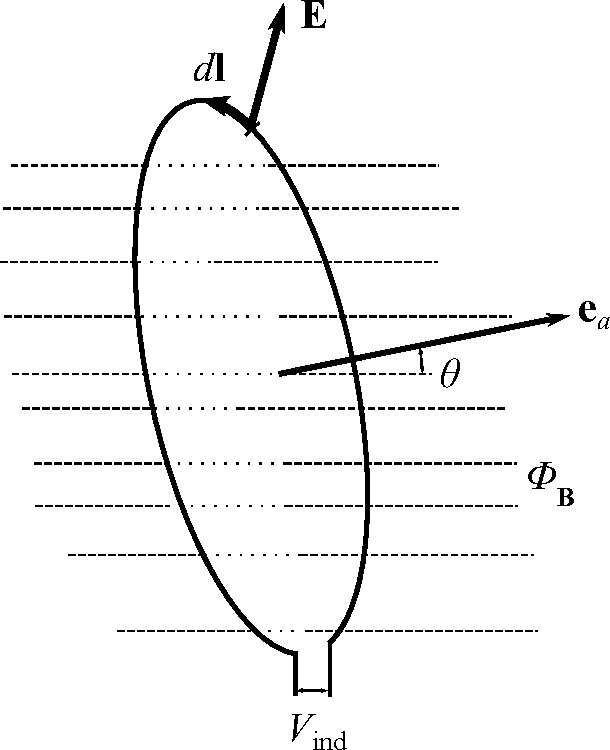
\includegraphics[width=5cm]{ch2/img/spira_singola.pdf}
	\caption{Single coil in field}
\end{marginfigure}
Under the hypothesys of an uniform EM field, using Maxwell's equations it is possible to derive potential difference induced in the coil:
\begin{equation}
\label{eq:tensioneindotta}
\vind = \oint\limits_{\diameter}\efield\cdot\mathbf{l} = -\dfrac{d\Phi_{\bfield}}{dt}
\end{equation}
where flux is:
\begin{equation}
\begin{array}{rcl}
\Phi_{\bfield} & = & \int\limits_{A_c} \bfield \cdot \hat{\mathbf{e}}_a dA \\
 & = & \magperm_0 H A \ccos{\theta}
\end{array}
\end{equation}
It is evident a cosine relation between field and axiis of the coil. The value of induced potential is maximum when the magnetic field $\hfield$ is orthogonal to the coil. $\theta$ is the angle between the field an the axis of the coil. Fusing two previous equations, we get:
\[
\vind = \magperm_0 A_c \dfrac{dH}{dt}
\]
that for our example:
\[
\vind = -j \omegaarva H A_c \magperm_0
\]
For conformity with the litterature, we express the magnetic field in terms of electric field\sidenote{It is known that: \newline $\magperm_{0} H = \dfrac{E}{\velocitaluce}$}:
\begin{equation}
\vind = \omegaarva \numerospire A_c \dfrac{E}{\velocitaluce}
\end{equation}

\myparagraph{Ferrite effect}
Inserting a ferrite bar brings to a deviation of the magnetic field flux. Fields lines are bended inside the ferrite because of its grater magnetic permeability
\begin{figure}
	\centering
	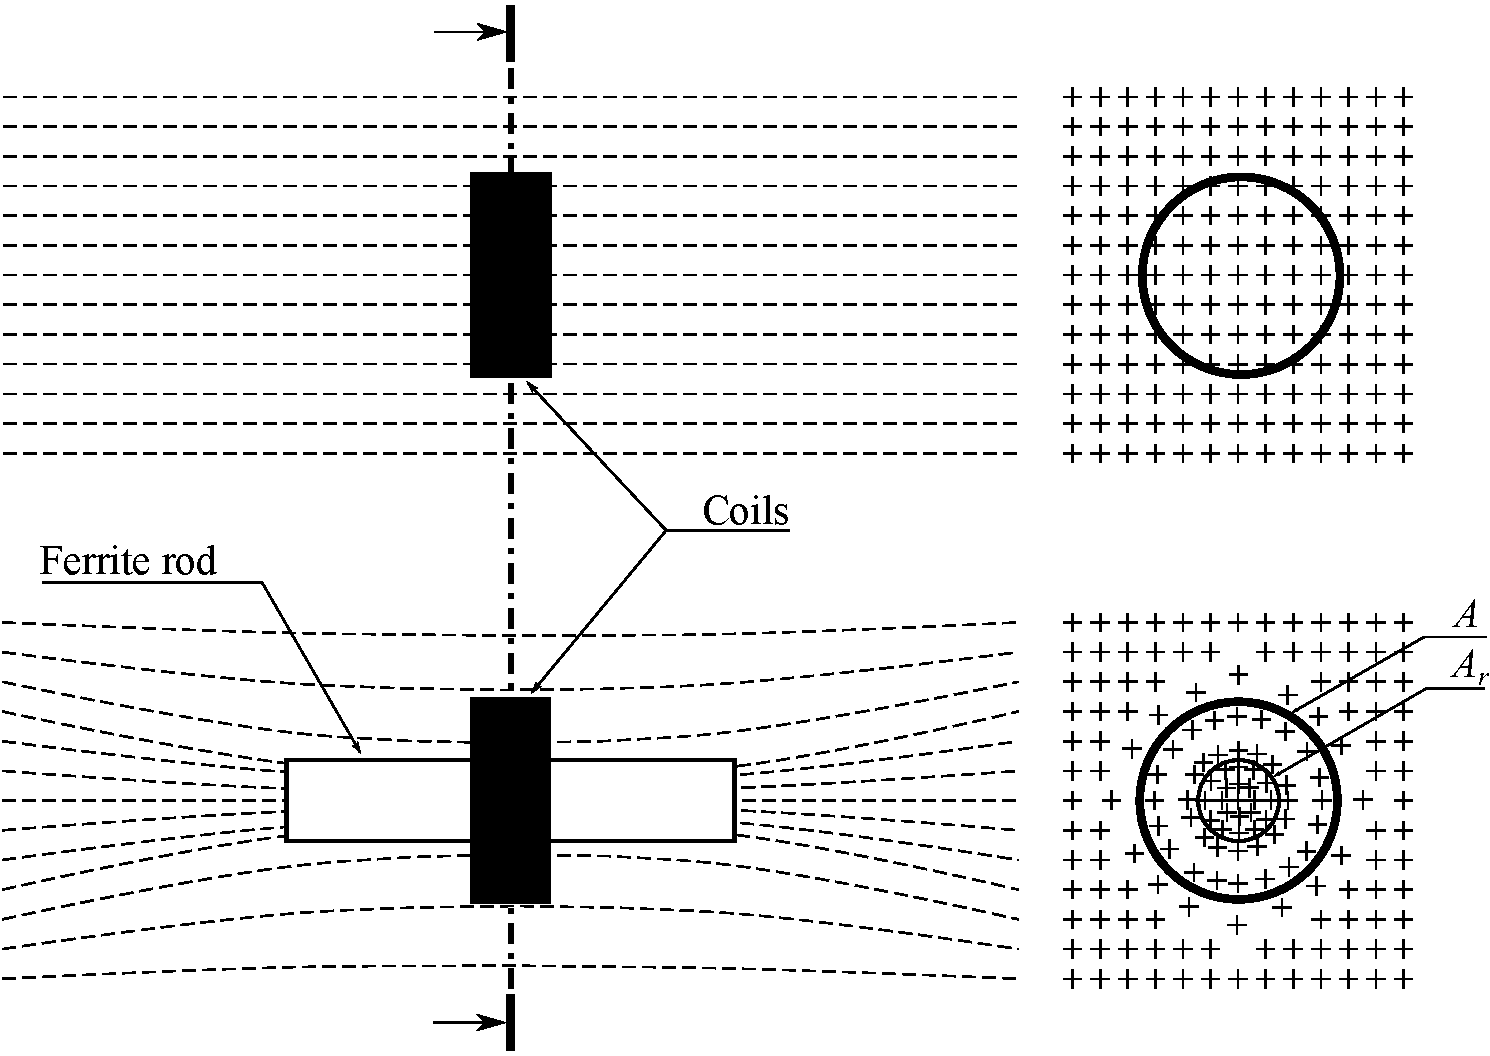
\includegraphics[width=11cm]{ch2/img/flux_lines.pdf}
	\label{fig:flussoferrite}
	\caption{Flux lines through coil and ferrite rod}
	\forceversofloat
\end{figure}
The total flux in section $A$ of figure \ref{fig:flussoferrite} is given by the flux that crosses area $A-A_r$ and flux that crosses area $A_r$:
\arraymath{
	\Phi_T & = & \Phi_{\bfield_1} + \Phi_{\bfield_2} \\
	\Phi_{\bfield_1} & = & \magperm_r A_r H \\
	\Phi_{\bfield_2} & = &\magperm_0 (A-A_r) H
}
and thus the total field is:
\begin{equation}
\Phi_T = H A_r \braces{ \magperm_r + \magperm_0 \braces{ \dfrac{A}{A_r} - 1} }
\end{equation}
bringing the previous equation in \ref{eq:tensioneindotta}, and simplifying with respect to constant parts of area, we get:
\begin{equation}
\vind = \omegaarva \numerospire \dfrac{E}{c} A_r \braces{\magperm_r + \braces{\dfrac{\diameter_c^2}{\diameter_r^2}-1}}
\end{equation}
In a real coil, we have a coil diameter that is equal to $\diameter_c = \diameter_c' + \diameter_\mathrm{wire}$, and it is usual to approximate $\diameter_c \approx \diameter_r$, and our antenna equation becomes:
\begin{equation}
\vind = \omegaarva \numerospire \dfrac{E}{c} A_r \magperm_r
\end{equation}
From which appears that the insertion of a ferrite rod in a coils inductance brings to an increase of induced tension proportional to the value of magnetic permeability of the ferrite itself. The identification of this value is not trivial and should be done experimentally. There are only some numerical approximation to the value of $\magperm_0$ related to the dimensions of ferrite bar, but it appears evidently a correlation between the ratio bar length/bar diameter. The greater this ratio, the greater the value of permeability\sidenote{We could give a trivial interpretation of this statement: the greater the length of the ferrite bar, the greater the number of flux lines that are bended into the bar; also the smaller the diameter, the grater the density of bended flux lines, thus the greater permeability value.}. 
\begin{equation}
\magperm_r \propto \dfrac{l_r}{\diameter_r}
\end{equation}

\myparagraph{Antenna effective height}
Effective height of antenna is defined as the ratio between the induced potential in the coils end the electric field intensity:
\begin{equation}
\altezzaeffettiva = \dfrac{\vind}{E}
\end{equation}
Applying previous equation to the definition of effective height:
\begin{equation}
\altezzaeffettiva = \dfrac{\omegaarva \numerospire A_r}{c} \braces{\magperm_r + \braces{\dfrac{\diameter_c^2}{\diameter_r^2}-1}}
\end{equation}

\subsection{Equivalent circuit and noise}
From a pure circuit point of view, ferrite antenna is seen as an an RLC circuit, in which we identify three passive components:
\begin{itemize}
\item $L\rightarrow\mathbf{Z}_L = j\omega L$: coil inductance
\item $R_p\rightarrow\mathbf{Z}_R = R_p$: wire resistance
\item $C\rightarrow\mathbf{Z}_C = (j\omega L)^{-1}$: parassite capacitance
\end{itemize}
The input voltage of the circuit is $\vind=\altezzaeffettiva E$
\begin{marginfigure}
	\centering
	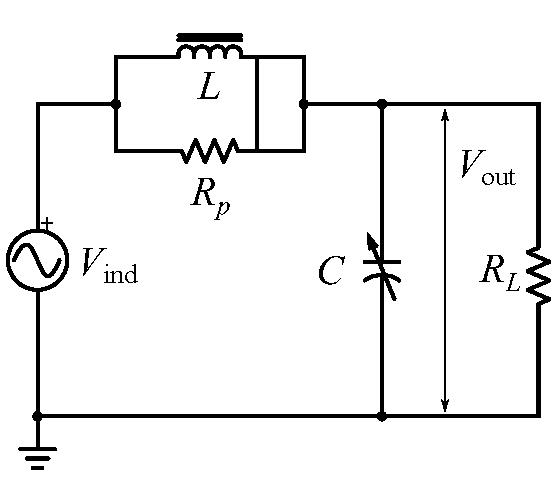
\includegraphics[width=5cm]{ch2/img/circuito_eq.pdf}
	\caption{Antenna equivalent circuit}
\end{marginfigure}

\myparagraph{Signal}
Starting from the definition of the equivalent circuit, with an external resistive load $R_L$ it is possible to derive a transfer function (full derivation in appendix at equation \ref{eq:transferfunc}):
\begin{equation}
\dfrac{V_{\mathrm{out}}}{\vind} = G(s) = \dfrac{\omega_{LC}}{Q_{\alpha}} \dfrac{s + Q_{\alpha} \omega_{LC}}{s^2 + \dfrac{\omega_{LC}}{Q_{\beta}} s + \omega_{LC}^2}
\end{equation}
\marginnote{\arraymath{
	\omega_{LC}^2 & = & \dfrac{1}{LC} \\
	Q_{\alpha} & = & \omega_{LC} R_P C \\
	Q_{\beta} & = & \omega_{LC} \dfrac{R_P R_L}{R_P + R_L} C
}}
if we obtain an $\omega_{LC} = \omegaarva$, we get resonance for an ARTVA incident signal: $s=j\omegaarva$:
\begin{equation}
G(j\omegaarva) = \left( -j Q_{\beta} \right) \left( 1 + \dfrac{j}{Q_{\alpha}} \right)
\end{equation} 
and then:
\begin{equation}
V_{\mathrm{out}} = \altezzaeffettiva \dfrac{Q_{\beta}}{Q_{\alpha}} E
\end{equation}

\myparagraph{Noise}
We could consider different sources of noise for our ferrite antenna:
\begin{itemize}
\item Boltzmann temperature noise
\item ferrite polarization noise
\item skin effect noise
\item auto-inductance noise
\end{itemize}

Even if some of those source are easily to model, some of them are not and require an experimental interpolation. For the Boltzmann withe noise:
\[
V_{n,B} = \sqrt{4 \boltzmann T \Delta f Q_{\beta} \mathbf{Z}_{L}}
\]
that is environment dependent. For the other sources, some more considerations must be driven. Skin effect and ferrite noise are proportional to the received field. 
Those two effects must be carefully taken into account and analyzed from experimental point of view. The first one is due to the distribution of the current in the section of the coil wire: current tends to accumulate in the skin layer of the wire, generating eddy currents that are sources of noise. To this effect, some special woven wire, like litz wire, should be used.
The second effect, ferrite noise, derives from the polarization of the magnetic crystal inside ferrite. To polarize the whole ferrite bar, some energy must be spent to move magnetic domain, and the movement of those domain generates a noise. This effect is strictly related to the quality of material and cannot be mitigated.
Auto-inductance noise is due to the current that is absorbed by the serial circuit of antenna and load. In a production of a prototype it is important that input of identification circuit has a very high impedance to reduce a generation of this current on antenna. Some high quality devices implement a secondary loop on the antenna that acts as a re-generator, that tries to null those parasitic currents effect.

It is straightforward now, that all those noise effect could be resumed in an unique interpolated expression $n \braces{\vind,T}$.

For simulation purpose it is possible to simulate this as Gaussian white noise as follows:
\begin{equation}
\sigma = N\braces{\mathbf{0}, V_{n,B}} + 10^{x} \abs{\vind} N\braces{\mathbf{0}, \Sigma}
\end{equation}
with $x$ a value that scales the proportional noise.
\section{Digital ARTVA prototype}
\begin{figure*}
	\centering
	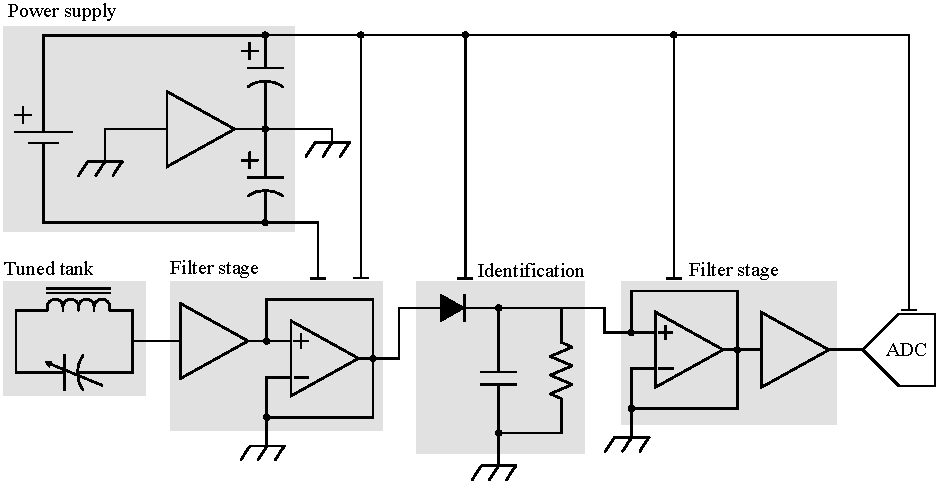
\includegraphics[scale=0.7]{ch2/img/block_circuit.pdf}
	\caption{Block diagram for the circuit}
	\label{fig:block_circuit}	
\end{figure*}
In the last section of this chapter, we use the knowledge collected to develop a prototype of an ARTVA receiver, in which there is not a transmission part. The receiver is the only fundamental module that we need for our drone, a transmitter will only be useless weight. 

In figure \ref{fig:block_circuit} there is the block outline of the device:
\begin{itemize}
\item the first block is the tuned tank, or tuned amplifier
\item the second block is the buffer and conditioner stage
\item the third block is the identification part
\item an amplification and a second buffer
\item digital component
\item dual supply stage
\end{itemize}
Through this section, each block will be discussed and explained. The design process has taken into account the tollerances for passive components\sidenote{Resistors: 5\%\newline Capacitors: 20\%}

\subsection{Tuned tank}
% \begin{figure}[b]
% 	\includegraphics[viewport=x y x y]{ch2/img/receiver3.pdf}
% 	\caption{}
% 	\label{fig:circuit}
% 	%\forceversofloat
% \end{figure}
\begin{figure}[h]
	\centering
	\includegraphics*[viewport=3 3 240 457,scale=0.4]{ch2/img/receiver3.pdf}
	\caption{Tuned tank portion of circuit}
	\label{fig:tunedtank}
	%\forceversofloat
\end{figure}

The tuned tank is composed by a ferrite antenna, with a rod of \num{10}\si{\centi\meter} per \diameter \num{1}\si{\centi\meter}. The wire of the coil is a \num{30} AWG enameled copper wire, with a final parasite resistance of \num{22}\si{\ohm}. The coil as \num{70} windings. For more informations about this tuned circuit, check previous section.

\subsection{Buffer and filter}
\begin{figure*}[h]
	\centering
	\includegraphics*[viewport=170 3 1250 380,scale=0.4]{ch2/img/receiver3.pdf}
	\caption{First filter stage}
	\label{fig:filter1}
	%\forceversofloat
\end{figure*}

This block is composed by a first stage that acts as a separation between the tuned tank and the filter, thus is also called voltage follower. To limit the number of components on the board this stage is obtained with an operational amplifier. To grant a longer receiving range, an high--gain selective active filter is in cascade to the buffer before the identification. It is important to select an operational amplifier with an high bandwidth--gain--product to grant the gain at \num{457}\si{\kilo\hertz}, at which the filter is centered. Also, this stage depends to the dual \num{\pm 5}\si{\volt} supply stage. 
\begin{marginfigure}
	\centering
	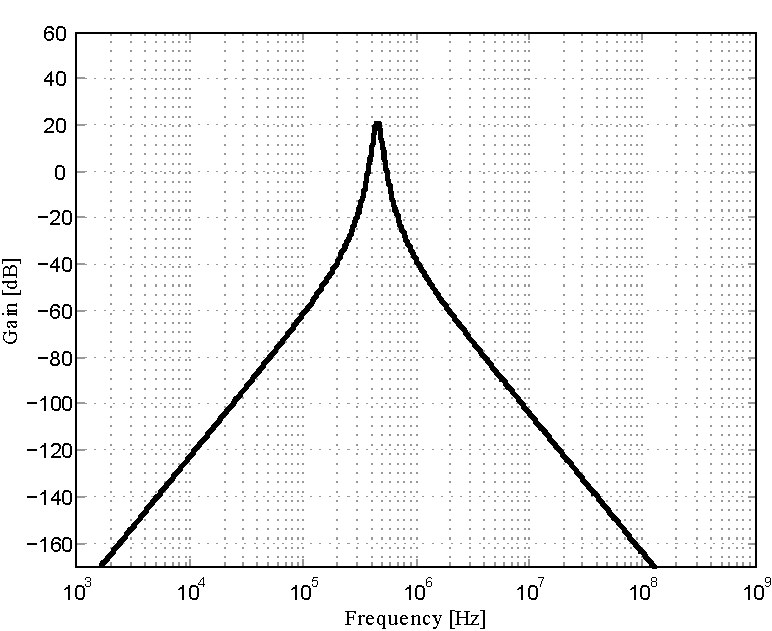
\includegraphics[width=5cm]{ch2/img/filter1.pdf}
	\caption{Filter magnitude characteristic}
\end{marginfigure}

The op--amp chosen is \texttt{LF347N}, even if a faster amplifier may be selected, it is advised to stay below the \num{60}\si{\mega\hertz} BW, to avoid auto--resonance effects.

\subsection{Identification}
\begin{figure}[h]
	\centering
	\includegraphics*[viewport=1251 3 1580 595,scale=0.4]{ch2/img/receiver3.pdf}
	\caption{Identification stage}
	\label{fig:identifier}
	%\forceversofloat
\end{figure}
\begin{marginfigure}
	\centering
	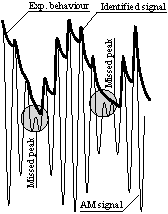
\includegraphics[width=4.5cm]{ch2/img/identificatore.pdf}
	\caption{Logical function of an identifier}
	\label{fig:identifier_log}
\end{marginfigure}
The central part of the circuit is an identification circuit, obtained with the monolithic classical IC \texttt{TA7641}\sidenote{A.k.a.: \texttt{MK484} or \texttt{ZN414}},  that acts as a one chip radio solution in AM. All receiver is derived from the modification of the basic circuit provided in schematics of this IC, extended with filtering and buffers, and the removal of the auto gain control resistance in the output feedback. Also, transistor amplification stage is removed. The output of this circuitry is in \numrange{40}{60}\si{\milli\volt}, with a very low current required. The input pin has a good impedance 

To better understand the use of this stage, look at figure \ref{fig:identifier_log}, in which an extremely simplified version of the IC is represented with common components. The IC straightens the received signal and identifies the envelope of the modulated intelligence with a low pass filter that has a dynamic not too slow, to not loose some of the higher frequencies information modulated (also called missed peak). IC implements this function with an high quality envelope detector.
\begin{figure*}[h]
	\centering
	\includegraphics*[viewport=1443 3 2320 350,scale=0.4]{ch2/img/receiver3.pdf}
	\caption{Low pass filter and amplification stage}
	\label{fig:filter2}
	\forceversofloat
\end{figure*}

\subsection{Amplifier}

The identified signal is, again, amplified and filtered, to a lower frequency, to grant the isolation of the square wave, with respect to the residual carrier and other source of interference. A \num{10}\si{\decibel} gain filter, with 2 stages was implemented. After the filter, another buffer connects analog circuitry with digital micro--controller.
\begin{marginfigure}
	\centering
	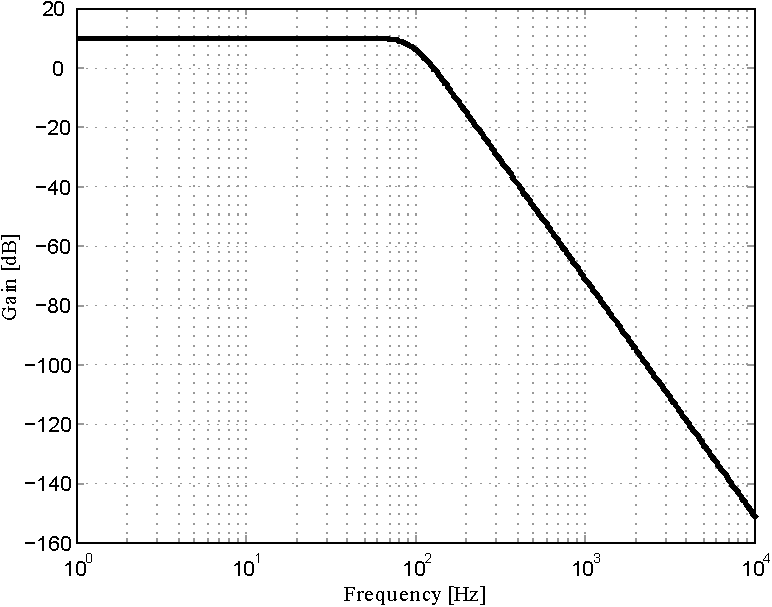
\includegraphics[width=5cm]{ch2/img/filter2.pdf}
	\caption{Filter magnitude characteristic}
\end{marginfigure}

\subsection{Digital stage}
\begin{figure}[h]
	\centering
	\includegraphics*[viewport=2320 3 2650 350,scale=0.4]{ch2/img/receiver3.pdf}
	\caption{Digital stage}
	\label{fig:adc}
	%\forceversofloat
\end{figure}
One last stage is he ADC and the UART interface on the micro--controller. Using an \texttt{MSP430} it is easy to develop in \texttt{C} the routines necessary to perform the task. To reduce the power consumption, ADC sampling is performed with ALU in power saving mode. Once the sampling task is completed, an interrupt brings up the ALU that set up the variables too be sent over serial interface UART (or SPI or I2C).

\subsection{Dual supply}
The supply is obtained through the use of a virtual ground and a symmetrical classical regulation circuit. This scheme is sometimes called rail splitter, and it is necessary for the first regulation stage, to avoid op--amps saturation.
\begin{figure}[h]
	\centering
	\includegraphics*[viewport=3 450 580 750,scale=0.4]{ch2/img/receiver3.pdf}
	\caption{Example of a sampling result}
	\label{fig:sampling_res}
	\forceversofloat
\end{figure}

\subsection{Tri--axes ARTVA}
In figure \ref{fig:sampling_res} there is an example of sampling from the real prototype, using MATLAB serial reading capabilities. A complete prototype uses three equal antenna--filter--identification--amplifier stage, with orthogonal antennas, and one single ADC micro--controller and power supply.
\begin{figure}[h]
	\centering
	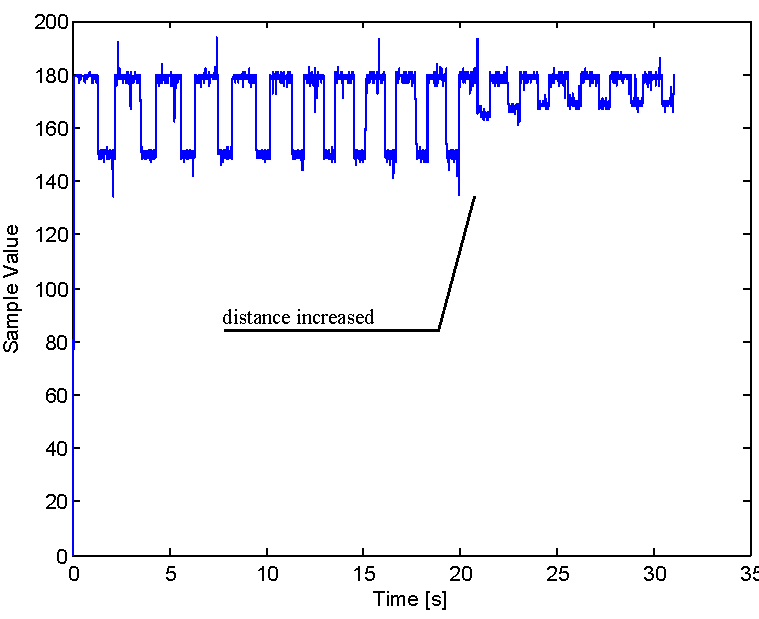
\includegraphics[scale=0.65]{ch2/img/sampling_result.pdf}
	\caption{Complete circuit}
	\label{fig:completecirc}
	%\forceversofloat
\end{figure}
\begin{figure}[p]
	\centering
	\includegraphics[scale=0.25,angle=90]{ch2/img/receiver3.pdf}
	\caption{Complete circuit}
	\label{fig:completecirc}
	\forceversofloat
\end{figure}

%\FloatBarrier
\clearpage
%%%%%%%%%% Appendix %%%%%%%%%%%%%%%%%%%%%%%%%%%%%%%%%%%%
% Appendix of chapter 2

\section{Appendix}

\subsection{Polar coordinates}

Maps:
\begin{equation} \left\{ \begin{array}{rcl} x & = & r \sin(\theta) \cos(\phi) \\ y & = & r \sin(\theta) \sin(\phi) \\ z & = & r \cos(\theta) \end{array}\right. \rightarrow \left\{ \begin{array}{rcl} r & = & \sqrt{x^2+y^2+z^2} \\ \theta & = & \arctan\left(\dfrac{z}{\sqrt{x^2+y^2}}\right) \\ \phi & = & \arctan\left( \dfrac{x}{y} \right) \end{array} \right. \end{equation}

Versors in Cartesian coordinates:
\begin{equation} \left[ \begin{array}{ccc} \vrr & \vrtheta & \vrphi \end{array}\right] = \dfrac{1}{\sqrt{x^2+y^2+z^2}} \left[ \begin{array}{ccc} x & \dfrac{xz}{\sqrt{x^2+y^2}} & -\dfrac{y}{\sqrt{x^2+y^2}} \\ y & -\dfrac{yz}{\sqrt{x^2+y^2}} & \dfrac{x}{\sqrt{x^2+y^2}} \\ z & -\dfrac{x^2+y^2}{\sqrt{x^2+y^2}} & 0 \end{array} \right] \end{equation}

\subsection{Evidences}

\myparagraph{EM field dynamic potential}
The following equations are the proof for \ref{eq:potvecmaxwell}
\begin{equation}
\begin{array}{rcl}
\nabla \cdot \left(  - \nabla \scpot - \partialtarg{\afield} \right) & = & \dfrac{\chargedens}{\dielettrico_0} \\
\nabla^2 \scpot + \partialt{\nabla \cdot \afield} & = & -\dfrac{\chargedens}{\dielettrico_0} \\
 & & \\
\magperm_0 \left( \currdens + \dielettrico_0 \partialt\left(- \nabla \scpot - \partialtarg{\afield}\right) \right) & = & \nabla \times \left( \nabla \times \afield \right) \\
\magperm_0 \currdens - \magperm_0 \dielettrico_0 \dfrac{\partial^2 \afield}{\partial t^2} - \magperm_0 \dielettrico_0 \nabla \dfrac{\partial \scpot}{\partial t} & = & \nabla \left( \nabla \cdot \afield \right) - \nabla^2 \afield \\
\nabla^2 \afield - \dfrac{1}{c^2} \dfrac{\partial^2 \afield}{\partial t^2} - \nabla \left( \nabla \cdot \afield + \dfrac{1}{c^2} \dfrac{\partial \scpot}{\partial t} \right) & = & - \magperm_0 \currdens
\end{array}
\label{eq:evidence1}
\end{equation}

In the following equation invariance with respect to recalibration map is showed:
\begin{equation}
\label{eq:prooftransformationmap}
\begin{array}{rcl}
\nabla \times \afield' & = & \nabla(\afield + \nabla \lorentz) \\
 & = & \nabla \times \afield + \nabla \times \nabla \lorentz \\
 & = & \nabla \times \afield \\
 & = & \bfield \\
 & & \\
- \nabla\scpot' - \partialtarg{\afield'} & = & -\nabla \left( \scpot - \partialtarg{\lorentz} \right) - \partialt\left( \afield + \nabla \lorentz \right) \\
 & = & -\nabla \scpot + \nabla \partialt \lorentz - \partialtarg{\afield} - \partialt\nabla\lorentz \\
 & = & -\nabla \scpot - \partialtarg{\afield} \\
 & = & \efield
\end{array}
\end{equation}

\myparagraph{Magnetic dipole radiation}
To evaluate the integral \ref{eq:integraledacalc}  we should consider some simplifications.

$r' \ll r$: for an ideal dipole, coils radius shall be really with respect to radio vector:
\[
\begin{array}{rcl}
\kappa & = & \sqrt{(\radiodist - \radiodist') \cdot (\radiodist - \radiodist')} = \\
 & = & \sqrt{\radiodist \cdot \radiodist + \radiodist' \cdot \radiodist' - 2\; \radiodist \cdot \radiodist'} \\
 & = & \sqrt{r^2 + r'^2 - 2\,r\,r'\,sin(\theta)cos(\varphi')} \\
 & = & r\;\sqrt{1 + \dfrac{r'^2}{r^2} - 2\,\dfrac{r'}{r}\,sin(\theta)cos(\varphi')}
\end{array}
\]
the simplification is performed by the use of Taylor expansions, under the hypothesis of $r'^2/r^2 \approx 0$:
\arraymath{
\kappa & = & \mathrm{Taylor}_2\left[ r\;\sqrt{1 - 2\,\dfrac{r'}{r}\,sin(\theta)cos(\varphi')} \right]_{\dfrac{r'}{r} \rightarrow 0} \\
 & \approx & r\left( 1 - \dfrac{r'}{r}\,sin(\theta)cos(\varphi') \right)
}
imposing the inverse:
\arraymath{
\dfrac{1}{\kappa} & = & \dfrac{1}{r}\left( 1 - \dfrac{r'}{r}\,sin(\theta)cos(\varphi') \right)^{-1} \\
 & = & \mathrm{Taylor}_2\left[ \dfrac{1}{r}\left( 1 - \dfrac{r'}{r}\,sin(\theta)cos(\varphi') \right)^{-1} \right]_{\dfrac{r'}{r} \rightarrow 0} \\
 & \approx & \dfrac{1}{r}\left( 1 - \dfrac{r'}{r}\,sin(\theta)cos(\varphi') \right)
}

$r' \ll \lambda = 2\pi\velocitaluce/\omegaarva$: this observation permits us to simplify the cosine in the argument of the integral, with $\tau$ as defined in \ref{eq:campidef1}:
\marginnote{$\cos(\gamma + \beta) = \cos\gamma\cos\beta - \sin\gamma\sin\beta$\\for $\gamma\rightarrow0$ we get $\ssin{\gamma} \approx \omegaarva\tau$ and $\ccos{\gamma} \approx 1$}
\arraymath{
\ccos{\omegaarva \left( t - \dfrac{\kappa}{\velocitaluce}\right)} & \approx & \ccos{\omegaarva\tau} + \dfrac{\omegaarva r'}{\velocitaluce} \ssin{\theta} \ccos{\varphi'} \\
 & = & \ccos{\omegaarva\tau}\ccos{\dfrac{\omegaarva r'}{\velocitaluce} \ssin{\theta} \ccos{\varphi'}} - \\
 &   & + \ssin{\omegaarva\tau} \ssin{\dfrac{\omegaarva r'}{\velocitaluce} \ssin{\theta} \ccos{\varphi'}} \\
 & \approx & \ccos{\omegaarva\tau} - \\ & & + \ssin{\omegaarva\tau} \ssin{\dfrac{\omegaarva r'}{\velocitaluce} \ssin{\theta} \ccos{\varphi'}}
}

The union of the two simplifications give us as integral argument:
\[\begin{array}{l}
\dfrac{1}{r}\braces{1+\dfrac{r' \ccos{\theta} \ssin{\varphi'}}{r}} \cdot \\
\cdot \braces{\ccos{\omegaarva\tau} - \dfrac{\omegaarva r' \ssin{\theta} \ccos{\varphi'}\ssin{\omegaarva\tau}}{\velocitaluce}}
\end{array}\]
expanding and considering $\xi = \ssin{\theta}\ccos{\varphi'}$ we obtain:
\[
\dfrac{1}{r} \braces{ \dfrac{\omegaarva\ssin{\omegaarva\tau}\xi r'}{c} + \ccos{\omegaarva\tau} - \dfrac{\omegaarva\ssin{\omegaarva\tau}\xi r'^2}{cr} + \dfrac{\ccos{\omegaarva\tau}\xi r'}{r} }
\]
where the term $\frac{r'^2}{cr} = \frac{r'}{r}\;\frac{\omegaarva}{2\pi}\;\frac{r'}{\lambda} \approx 0$ as we have already stated:
\[
\dfrac{1}{r} \braces{ \ccos{\omegaarva\tau} -\braces{\dfrac{\omegaarva}{c}\ssin{\omegaarva\tau} - \dfrac{1}{r}\ccos{\omegaarva\tau}}r'\xi}
\]
extracting only the parts that are function of integration variable $\varphi'$:
\arraymath{
a_1 & = & \dfrac{1}{r} \ccos{\omegaarva\tau} \\
a_2 & = & \dfrac{1}{r} \braces{\dfrac{\omegaarva}{c}\ssin{\omegaarva\tau} - \dfrac{1}{r}\ccos{\omegaarva\tau}}r'\ssin{\theta}
}
The final integral is in the form:
\[
\afield(\radiodist,t) = \dfrac{\magperm_0 J_0 r'}{4\pi r} \int\limits_{0}^{2\pi}a_1 \ccos{\varphi'} - a_2 \cos^2\braces{\varphi'} d\varphi' \hat{\phi}
\]
and thus solved:
\marginnote{$\begin{array}{l} \int\limits_0^{2\pi}\ccos{\varphi'}d\varphi' = 0 \\ \int\limits_0^{2\pi}\cos^2\braces{\varphi'}d\varphi' = \pi \end{array}$}
\arraymath{
\afield(\radiodist,t) & = & -\dfrac{\magperm_0 J_0 r'}{4\pi} \pi a_2 \\
 & = & \dfrac{\magperm_0 J_0 r'^2 \pi}{4\pi r} \braces{\dfrac{1}{r}\ccos{\omegaarva\tau} - \dfrac{\omegaarva}{c}\ssin{\omegaarva\tau}}
}
Applying the substitution $m_0 = \pi r'^2 J_0$ we found the solution reported in equation \ref{eq:soluzioneint}.

\myparagraph{Complex version of magnetic field}
Here the proof of complex magnetic field equations:
\[
\begin{array}{rcl}
B_r & = & \dfrac{1}{2} \dfrac{\magperm_0 m_0}{\pi} \ccos{\theta} \braces{\dfrac{1}{r^3}\ccos{\omegaarva \tau} - \dfrac{\kappa}{r^2} \ssin{\omegaarva \tau}} \\
 & = & \dfrac{1}{2} \dfrac{\magperm_0 m_0}{\pi} \ccos{\theta} \kappa^3 \braces{ \dfrac{1}{r^3 \kappa^3} \ccos{\omegaarva\tau} - \dfrac{1}{r^2 \kappa^2} \ssin{\omegaarva\tau} } \\
 & = & \dfrac{1}{2} \dfrac{\magperm_0 m_0}{\pi} \ccos{\theta} \kappa^3 \braces{ \dfrac{1}{r^3 \kappa^3} + \dfrac{j}{r^2 \kappa^2}} e^{j\omegaarva \tau} \\
 & = & \dfrac{1}{2} \dfrac{\magperm_0 m_0}{\pi} \ccos{\theta} \kappa^3 \braces{ \dfrac{j}{r^2 \kappa^2} + \dfrac{1}{r^3 \kappa^3}} e^{j\omegaarva \tau} \\
 & = & -\dfrac{1}{2} j \dfrac{\magperm_0 m_0}{\pi} \kappa^3 \ccos{\theta} \braces{\dfrac{1}{j^2 r^2 \kappa^2} + \dfrac{1}{j^3 r^3 \kappa^3}} e^{j\omegaarva \tau}
\end{array}
\]

\[
\begin{array}{rcl}
B_{\theta} & = & \dfrac{1}{4} \dfrac{\magperm_0 m_0}{\pi r^3 c^2} \ssin{\theta} \braces{\braces{\velocitaluce^2 - \omegaarva^2 r^2}\ccos{\omegaarva \tau} - \omegaarva r \velocitaluce \ssin{\omegaarva \tau}} \\
 & = & \dfrac{1}{4} \dfrac{\magperm_0 m_0}{\pi} \ssin{\theta} \braces{ \braces{\dfrac{1}{r^3}-\dfrac{\omegaarva^2}{c^2 r}}\ccos{\omegaarva \tau} - \dfrac{\omegaarva}{r^2 c} \ssin{\omegaarva \tau}} \\
 & = & \dfrac{1}{4} \dfrac{\magperm_0 m_0}{\pi} \ssin{\theta} \braces{ \braces{\dfrac{1}{r^3}-\dfrac{\kappa^2}{r}}\ccos{\omegaarva \tau} - \dfrac{\kappa}{r^2} \ssin{\omegaarva \tau}} \\
 & = & \dfrac{1}{4} \dfrac{\magperm_0 m_0}{\pi} \ssin{\theta} \kappa^3 \braces{ \braces{\dfrac{1}{r^3 \kappa^3}-\dfrac{1}{r \kappa}}\ccos{\omegaarva \tau} - \dfrac{1}{r^2 \kappa^2} \ssin{\omegaarva \tau}} \\
 & = & \dfrac{1}{4} \dfrac{\magperm_0 m_0}{\pi} \ssin{\theta} \kappa^3 \braces{ \braces{\dfrac{1}{r^3 \kappa^3}-\dfrac{1}{r \kappa}} + \dfrac{j}{r^2 \kappa^2}} e^{j\omegaarva \tau} \\
 & = & \dfrac{1}{4} \dfrac{\magperm_0 m_0}{\pi} \ssin{\theta} \kappa^3 \braces{-\dfrac{1}{r \kappa} + \dfrac{j}{r^2 \kappa^2} + \dfrac{1}{r^3 \kappa^3}} e^{j\omegaarva \tau} \\
 & = & -\dfrac{1}{4} j \dfrac{\magperm_0 m_0}{\pi} \kappa^3 \ssin{\theta} \braces{\dfrac{1}{j r \kappa} + \dfrac{1}{j^2 r^2 \kappa^2} + \dfrac{1}{j^3 r^3 \kappa^3}} e^{j\omegaarva \tau}
\end{array}
\]

\myparagraph{The field in cartesian coordinates}
From the figure \ref{fig:polar2cartesian} we derive the following relations:
\arraymath{
\vers{r} & = & \dfrac{\radiodist}{\abs{\radiodist}} \\
\vrtheta & = & \dfrac{ (\magdipole \times \radiodist) \times \radiodist }{ \abs{ (\magdipole \times \radiodist) \times \radiodist } } 
}
and the magnetic dipole vector is the projection on the two versors:
\arraymath{
\magdipole \cdot \vers{r} & = & m_0 \ccos{\theta}\\
\magdipole \cdot \vrtheta & = & -m_0 \ssin{\theta}
}
thus equation \ref{eq:magneticfieldpolar} becomes:
\arraymath{
\bfield & = & \dfrac{\magperm_0}{4 \pi r^3} \braces{ 2 m_0 \ccos{\theta} \vers{r} + m_0 \ssin{\theta} \vrtheta } \\
 & = & \dfrac{\magperm_0}{4 \pi r^3}\braces{2\braces{\magdipole \cdot \vers{r}} \vers{r} - \braces{\magdipole \cdot \vrtheta} \vartheta} \\ 
 & = & \dfrac{\magperm_0}{4 \pi r^3}\braces{3\braces{\magdipole \cdot \vers{r}} \vers{r} - \braces{\magdipole \cdot \vers{r}} \vers{r} - \braces{\magdipole \cdot \vrtheta} \vartheta} \\ 
 & = & \dfrac{\magperm_0}{4 \pi r^3}\braces{3\braces{\magdipole \cdot \vers{r}} \vers{r} - \magdipole}
}
putting the last equation in an analytical math engine, we derive this compact version, using as notation $\radiodist = [x,\,y,\,z]^T$:
\begin{equation}
\bfield = \dfrac{\magperm_0}{4 \pi r^5} \magfieldmatrix \magdipole
\end{equation}

\subsection{Antenna transfer function}
It is easy to derive transfer function, if we consider the system as a voltage divider:
\begin{equation}\label{eq:transferfunc}
\begin{array}{ccl}
\dfrac{V_{\mathrm{out}}}{\vind} & = & \dfrac{\left(R_L \parallel C s \right)}{\left(R_L \parallel C s \right) + \left(R_P \parallel L s \right)} \\
& = & \dfrac{\dfrac{1}{\dfrac{1}{R_L} + Cs}}{\dfrac{1}{\dfrac{1}{R_L} + Cs} + \dfrac{1}{\dfrac{1}{R_L} + \dfrac{1}{L s}}} \\
& = & \dfrac{ \dfrac{1}{R_p}+\dfrac{1}{Ls} }{ \dfrac{1}{R_L} + Cs + \dfrac{1}{R_P} + \dfrac{1}{Ls} } \\
& = & \dfrac{1}{R_P C} \dfrac{s + \dfrac{R_P}{L}}{s^2 + \dfrac{1}{C \dfrac{R_P R_L}{R_P + R_L}}s + \dfrac{1}{LC}} 
\end{array}
\end{equation}



	\chapter{Drone Avionics}
\minitoc
\thispagestyle{plain}

\renewcommand{\arraystretch}{1.75}

In this chapter we explore the searching algorithm applied to a dynamic simulated device really close to our drone. The simulation will use a simpler control model (LQR) and will implement the perception action paradigm for the searching part. Searching part will be performed with device implemented in previous chapter, with auxiliary range finder for obstacle avoidance and altitude keeping. All those elements build what is called avionic framework of the drone. The basic idea is to create a stacked structure that could be easily expanded in future; again, what we are discussing in an initial platform that could be improved with the use of more increasingly complex sensor--fusion, that allows to exploit the most sophisticated searching algorithm possible. 

\section{Perception Action paradigm}
The perception--action (PA) paradigm has a very strict connection with the definition of our searching algorithm. Lets try to understand what this paradigm is.

\subsection{The basic paradigm}
A PA map consider an agent in which external stimuli derive from a sensor network, that perform the perception section of the agent. Perception is therefore translated into a symbol that could be handled by the action section of the agent.
\begin{figure}[h]
\caption{Classical percetion--action map}
\centering
\begin{tikzpicture}[auto, node distance=2cm,>=latex']
	\node[input] (input) {};
	\node[block,right of=input] (perception) {Perception};
	\node[block,right of=perception] (action) {Action};
	\node[output, right of=action] (output) {};

	\draw[->] (input) -- node[pos=0.2] {Sensors} (perception);
	\draw[->] (perception) -- (action);
	\draw[->] (action) -- node[pos=0.7] {Actuators} (output);
\end{tikzpicture}
\end{figure}

Making a straight example on our device: we consider as sensor elements our digital ARTVA; the input to the perception stage, should be analyzed to perform an action, that is the movement of the drone towards buried position.

The relationship between the agent and the environment is called \emph{situatedness}, while the intercourse within what represents the \emph{body} on what represents the \emph{mind} of the agent is called \emph{embodiment}, as explained in \citep{thedynamicsofactivecaterogicalperception}.
\begin{marginfigure}
\centering
\begin{tikzpicture}[auto, node distance=1cm,>=latex']
	\node [rectangle, draw=black, minimum width=5cm,minimum height=3cm] (envir) {};
	\node [rectangle, draw=black, minimum width=3cm,minimum height=2.25cm] (body) at ++(0.75cm,-0.25cm) {};
	\node [rectangle, draw=black, dashed, minimum width=1.5cm,minimum height=1.5cm] (body) at ++(1.25cm,-0.5cm) {};
	\node [rectangle, fill=white] (situatedness) at ++(-0.75cm,-0.65cm) {$\underset{situatedness}{\longleftrightarrow}$};
	\node [rectangle, fill=white] (embodiment) at ++(.5cm,-0.85cm) {$\underset{embodiment}{\longleftrightarrow}$};
	\node [rectangle, fill=white, draw=black] at ++(-1.25cm,1.5cm) {\textbf{Environment}};
	\node [rectangle, fill=white, draw=black] at ++(1.5cm,0.85cm) {\textbf{Agent}};
	\node at(-0.3cm,0.6cm) {Body};
	\node at(1cm,0cm) {Mind};
\end{tikzpicture}
\caption{Embodiment and situatedness}
\end{marginfigure}

\subsection{Exploiting more complex behavior}
\myparagraph{Expanding PA}
Apart the basic behavior, the advantages of PA maps are related too the implementation of extremely complex actions using other techniques such as:
\begin{itemize}
\item subsumption and grounding
\item innate knowledge
\item bootstrapping
\item historical knowledge
\item shared knowledge
\end{itemize}
All those element could be serially implemented, one after the other, while they run together to create a coherent attitude with respect to the problem. One of the advanced feature that we will use in this project is the subsumption and the grounding of the symbols.

\myparagraph{Subsumption and grounding}
The \emph{symbols grounding} is an implementation of the embodiment of the agent as a stacked architecture in which different layer (subsumption), that performs different operations, are piled up in such a way that higher level, of higher complexity, could transparently use lower levels (symbols grounding \citep{harnad1990symbolgrounding}), and incorporate them to reach more complex behavior.
\begin{marginfigure}
\begin{tikzpicture}[auto, node distance=2cm,>=latex']

	\matrix [draw=white, row sep=0.1cm, column sep=1.5cm] {	
	   	& \node [block, right, anchor=west, text width=1.5cm, minimum width=1.5cm] (levelD) {Level 3}; & \\
		& \node [block, right,anchor=west, text width=1.8cm, minimum width=1.8cm] (levelC) {Level 2}; & \\
	 	& \node [block, right,anchor=west, text width=2.1cm, minimum width=2.1cm] (levelB) {Level 1}; & \\
		\node [input,right] (input) {}; & \node [block,anchor=west, text width=2.4cm, right, minimum width=2.4cm] (levelA) {Level 0}; & \node[output](output){} ; \\
 	};

	\draw [->] (input) -- node[below](mid) {Sensors} (levelA);
	\draw [->] (mid) |- node {} (levelB);
	\draw [->] (mid) |- node(midU) {} (levelC);
	\draw [->] (mid) |- node (midUb)  {} (levelD);
	\draw [->] (levelA) -- node[below] (midA) {Actuators} (output);
	\draw [->] (levelB) -| node[pos=0.3] (midB) {} (midA);
	\draw [->] (levelC) -| node[pos=0.3] (midC) {} (midB.south);
	\draw [->] (levelD) -| node[pos=0.3] (midD) {} (midC.south);

	\draw [->,dashed] (midUb.south) -- node  {} ++(0,0.8);
	\draw [<-,dashed] (midD.south) -- node {} ++(0,0.8);
\end{tikzpicture}
\caption{Subsumption and grounding architecture}
\end{marginfigure}

As an example, the very basic level that could be implemented is a stabilization control, that could be used to keep the plant in a controllable state. From this layer, an upper tracking layer will try to reduce the input error using the lower layer to preserve a safe stability for the system.

This techniques, introduced in \citep{layeredmobilerobot}, will be used in our avionics definition.

\myparagraph{Innate knowledge and emulation}
Evolution and generalization of the map are referred to the embodiment, with the implementation of an innate knowledge, that may be used to perform an internal emulation of the perceived environment. A typical example of this is the co--driver model implemented in \citep{artificialcodriver}, where emulation, defined as a mathematical model, is used to infer driver actions.

This techniques is also implemented in our avionics.
\begin{figure}[h]
\centering
\caption{Emulation in an agent}
\forceversofloat
\begin{tikzpicture}[auto, node distance=2.7cm,>=latex']
	% EMULATION
	\matrix[draw=black, row sep=0.1cm, column sep=0.2cm] (emulator) {
	 \node {\scriptsize{Model}}; \\ 
	 \node {\scriptsize{Hypothesis}};  \\
	};
	\node[above of=emulator] at ++(0,-1.8cm) {Emulator};

	% GROUNDING
	\matrix [draw=black,minimum width=4cm, minimum height=2.5cm, row sep=0.1cm, column sep=1cm, above of=emulator] (grounding) at ++(0,0cm) {	
		& \node [block, right,anchor=west, minimum width=1cm ,minimum height=0.5cm] (levelC) {}; & \\
	 	& \node [block, right,anchor=west, minimum width=1.25cm ,minimum height=0.5cm] (levelB) {}; & \\
		\node [input,right] (input) {}; & \node [block,anchor=west, right, minimum width=1.5cm, minimum height=0.5cm] (levelA) {}; & \node[output](output){} ; \\
 	};
	\node[above of=grounding] at ++(0,1.5cm) {Grounding};

	% EMULATOR
	\node[block,below of=emulator] (environment) at ++(0,1.2cm) {\textbf{Environment}};


	\draw [->] (input) -- node[below](mid) {} (levelA);
	\draw [->] (mid) |- node (midK) {} (levelB);
	\draw [->] (mid) |- node(midU) {} (levelC);
	
	\draw [->] (levelA) -- node[below] (midA) {} (output);
	\draw [->] (levelB) -| node[pos=0.3] (midB) {} (midA);
	\draw [->] (levelC) -| node[pos=0.3] (midC) {} (midB.south);


	\draw [->,dashed] (mid) -- node  {} ++(0,1.8);
	\draw [<-,dashed] (midC.south) -- node {} ++(0,0.5);

	\node[right of=grounding] (gr) {};
	\node[left of=grounding] (gl) {};

	\draw [->] (emulator.west) -|  (gl.south) |- (grounding);
	\draw [<-] (emulator.east) -|  (gr.south) |- (grounding);

	\node[block,minimum width=6cm, minimum height=5.25cm,dashed] (agent) at ++(0,1.9cm) {};
	\node[above of=agent] at ++(0,2cm) {\textbf{Agent}};

	\draw [<-] (environment.east) -- ++(2.5cm,0) |- (grounding);
	\draw [<-] (environment.west) -- ++(-2.5cm,0) |- (grounding);

\end{tikzpicture}
\end{figure}

\myparagraph{Bootstrapping and more}
In this paragraph, for completeness, we could cite other techniques that generalize embodiment and situatedness. One of the most recent generalization approach is called \emph{bootstrapping}. From \citep{sun2001implicit} and \citep{hierarchicalbootstrapping}, a cognitive system should identify and define its motion primitives\marginnote{Even if this procedure is clearly different from innate knowledge, the implementation of this technique do not exclude the implementation of some kind of innate knowledge.}. 

The exploration of motion domain is performed through the use of random inputs and fuzzy logic\citep{aframeworkforhierarchicalperceptionaction} on perception:
\begin{itemize}
\item random exploration gives an initial model for the primitives
\item repetition on the primitives allows the system to remove redundancies
\item further repetition remove unused parameters
\item last repetitions allows to perform an optimization and update of the model parameters
\end{itemize}

\section{Building the PA map of the drone}

\subsection{Overview of our searching map}

In figure \ref{fig:genPAmap} a comprehensive version of the map is presented. The map shows a tri--dimensional evolution in the upper side, where two different aims are achieved. One one side we have the searching for the signal, and on the other side we have the searching for the signal source. This particular design in the map was implement to grant to the avionics the ability to perform a sort of reasoning and reach a multiple objective, as it will be explained later on.

The drone has a complex control system, already implemented in IMU shield, that takes in consideration a linearized feedback that feeds an LQR control loop\citep{belanger1995control}. 

The system could be modified to solve a tracking problem, that will be used by the upper level. The tracking problem uses transparently the stabilization layer and it is used by the searching layer.

Upper layers, obstacle avoiding and altitude keeping, preserve drone to collide with isolated obstruction and at an altitude that is safe for rescuers. 
\begin{figure}[h]
	\centering
	%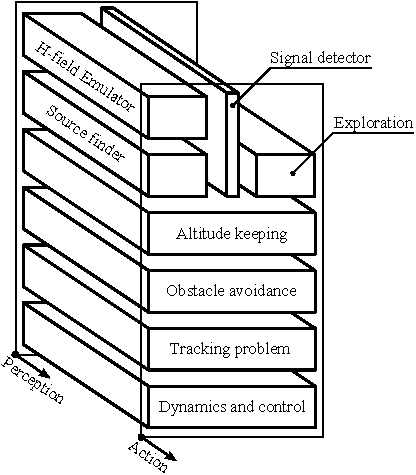
\includegraphics[scale=0.9]{ch3/img/PA_map_general.pdf}

	\begin{tikzpicture}[>=latex']
		\drawplanexy{-0.3}{-0.3}{-0.3}{6.7}{10}{dashed}{perception}
		\node [at=(perception_D),xshift=30,yshift=-10] {\textbf{Perception}};
		\drawcube{0}{0}{5}{6.4}{1}{white}{dinamica}{Dynamics and control}{};
		\drawcube{0}{1.2}{5}{6.4}{1}{white}{tracking}{Tracking Problem}{};
		
		\drawcube{0}{2.4}{5}{6.4}{1}{white}{ostacoli}{Obstacle Avoidance}{};
		\drawcube{0}{3.6}{5}{6.4}{1}{white}{altitude}{Altitude Keeping}{};
		
		\drawcube{0}{4.8}{5}{3}{1.5}{white}{source}{Source searching}{text width=2cm,align=center};
		\drawcube{0}{6.5}{5}{3}{1.5}{white}{emulatore}{Emulation}{text width=2cm,align=center};

		\drawplanezy{3.2}{4.8}{5}{4.5}{radar_det}{fill=white,opacity=0.90}{Radar detect}{rotate=45,xslant=1};

		\drawcube{3.4}{4.8}{5}{3}{3.2}{white}{alpha}{Exploration routines}{text width=2cm,align=center};
		\drawplanexy{-0.3}{-0.3}{5.3}{6.7}{10}{dashed}{action}
		\node [at=(action_D),xshift=20,yshift=-10] {\textbf{Action}};

		\draw [->,line width=1.5] (action_D) -- ++(0,0,2);
		\draw [->,line width=1.5] (perception_D) -- ++(0,0,2);

		\coordinate [at=(radar_det_D), yshift=-20] (arrows_point);
		\draw [->,dashed]  (arrows_point) -- ++(1.5,0,0); 
		\draw [->,dashed]  (arrows_point) -- ++(-1.5,0,0); 
	\end{tikzpicture}
	\forcerectofloat
	\caption{General Perception--Action map for our drone}
	\label{fig:genPAmap}
\end{figure}
\FloatBarrier
\section{Hexa--copter model}

The drone could be modeled with dynamical equations. The derivation of those equation will be performed from force analysis and control scheme is derived. A \texttt{C} version of the model, to be used in simulations is presented.

\subsection{Motion equations}
The system is governed by Euler--Newton equations, simplified with the imposition of the center of motion for Euler equations in center of mass of the drone. With character $g$ we refer to global coordinate system, while with $b$ we identify the coordinate system, that is attached to body and has origin in CoM:
\begin{equation}
\left\{
\begin{array}{rcl}
\totforcehexa_g & = & \massadrone \ddot{\hexastate}_g \\
\tottorquehexa_g & = & \dot{\mathbf{K}}_g + \dot{\hexastate}_g \times \mathbf{Q}_g%
\end{array}
\right.  \rightarrow  \left\{
\begin{array}{rcl}
\totforcehexa_b & = & m \mathbf{a}_b \\
\tottorquehexa_b & = & \dot{\mathbf{K}}_b%
\end{array}
\right.
\end{equation}
\myparagraph{External force and torque analysis}
There are several force that act on the body of the drone:
\begin{equation}
\totforcehexa_b = \sum\limits_{\mathrm{external}} F_b
\end{equation}

\textbf{Weight}:
\begin{equation}
\mathbf{P}_g = \vettore{0 \\ 0 \\ - m g}
\end{equation}

\textbf{Motor thrust}:
\begin{equation}
\mathbf{L}_b = \sum\limits_{i=1}^6 \vettore{0 \\ 0 \\ -L_{b,i}}
\end{equation}

\textbf{Total force}:
\begin{equation}
\totforcehexa_b = \vettore{\sin(\theta) \\ -\sin(\phi)\cos(\theta) \\ - \cos(\phi)\cos(\theta)} m g + \vettore{ 0 \\ 0 \\ - \sum\limits_{i=1}^6 L_{b,i}}
\end{equation}

For what concerns total external torque applied to the system:
\begin{equation}
\tottorquehexa_{b,\mathbf{0}} = \sum\limits_{\mathrm{external}} M_b + \sum\limits_{\mathrm{external}} (\mathbf{p}_b - \mathbf{0}) \times \totforcehexa_b
\end{equation}

\textbf{Thrust torque}, with $l$ distance between center of propeller and CoM
\begin{equation}
\mathbf{M}_b = \sum\limits_{i=0}^5 \vettore{ l \cos(i \pi/3) \\ l \sin(i \pi /3) \\ 0 } \times \mathbf{L}_{b,i}
\end{equation}

\textbf{Drag torque}, with $\beta$ the proportional factor between thrust and drag torque
\begin{equation}
\mathbf{D}_b = \sum\limits_{i=1}^6 \vettore{ 0 \\ 0 \\ \beta L_{b,i}}
\end{equation}

In general, the total torque is:
\begin{equation}
\tottorquehexa_{b,0} = \left[ \begin{array}{c}
-\dfrac{\sqrt{3}}{2} l \left( L_2 +L_3 - L_5 - L_6 \right) \\
\dfrac{1}{2} l \left( 2 L_1 + L_2 -L_3 - 2 L_4 - L_5 + L_6 \right) \\ 
\beta \left( L_1 - L_2 + L_3 - L_4 + L_5 - L_6 \right)
\end{array}
\right]
\end{equation}

\myparagraph{Inertial analysis}
We could define speed vector in body system of coordinates:
\begin{equation}
\vettore{\dot{x} \\ \dot{y} \\ \dot{z}} = \rotmat \vettore{u\\v\\w}
\end{equation}
\marginnote{The rotational matrix form body to ground is obtained through a sequence of elementary rotations:
${\mathcal{R} = \mathcal{R}_z(\psi)\;\mathcal{R}_y(\theta)\;\mathcal{R}_x(\phi)}$}.  that allows us to define the accelerations vector in the form:
\begin{equation}
\mathbf{a}_b = \dot{\mathbf{v}}_b + \boldsymbol{\omega}_b \times \mathbf{v}_b
\end{equation}
The relation that connects angular ratios in body coordinates and ground coordinates are derived from the so called \emph{Gimball's relations}\sidenote{Just a clarification on the notation used. Square parentheses $[\cdot]$ identifies vector element that belongs to the same basis, while vectorial elements in curly brackets $\{\cdot\}$ do not share the same basis}:
\begin{equation}
\boldsymbol{\omega}_b = \mathcal{R}_x (\phi) \dot{\phi} \vers{e}''_x + \mathcal{R}_x(\phi) \mathcal{R}_y(\theta) \dot{\theta} \vers{e}'_y + \mathcal{R}_x(\phi) \mathcal{R}_y(\theta) \mathcal{R}_z(\psi) \dot{\psi} \vers{e}_z
\end{equation}
that is simplified in the matrix form:
\begin{equation*}
\left[ \begin{array}{c} p \\ q \\ r \end{array} \right] = \left[ \begin{array}{ccc}
 1 & 0 & -\sin(\theta) \\
 0 & \cos(\phi) & \sin(\phi)\cos(\theta) \\
 0 & -\sin(\phi) & \cos(\phi)\cos(\theta)
 \end{array} \right] \left\{ \begin{array}{c} \dot{\phi} \\ \dot{\theta} \\ \dot{\psi} \end{array} \right\}
\end{equation*}
that through inversion gives:
\begin{equation}
\left\{ \begin{array}{c} \dot{\phi} \\ \dot{\theta} \\ \dot{\psi} \end{array} \right\} = 
\left[ \begin{array}{ccc}
 1 & \dfrac{\sin(\phi) \sin(\theta)}{\cos(\theta)} &  \dfrac{\cos(\phi) \sin(\theta)}{\cos(\theta)}\\
 0 & \cos(\phi) & -\sin(\phi) \\
 0 & \dfrac{\sin(\phi)}{\cos(\theta)} & \dfrac{\cos(\phi)}{\cos(\theta)} 
 \end{array} \right]
\left[ \begin{array}{c} p \\ q \\ r \end{array} \right]
\end{equation}
For what concerns angular inertia in body reference frame:
\begin{equation}
\begin{array}{rcl}
\dot{\mathbf{K}}_b &=& \matriceinerzia \dot{\boldsymbol{\omega}}_b + \boldsymbol{\omega}_b \times \matriceinerzia \boldsymbol{\omega}_b \\
&=& \left[ \begin{array}{c} I_x \dot{p} \\ I_y \dot{q} \\ I_z \dot{r} \end{array} \right] + \left[ \begin{array}{c} (I_z-I_y) q r \\ (I_x-I_z) p r \\ (I_y-I_x) p q \end{array} \right]
\end{array}
\end{equation}

\myparagraph{Newton--Euler equations}
Defined state vectors and control vectors:
\arraymath{%
\hexastate & = & \left[ x,y,z,u,v,w,\phi,\theta,\psi,p,q,r \right]^T \\
\hexacontrol & = & \left[ L_1, L_2, L_3, L_4, L_5, L_6 \right]^T%
}
we get the following Newton--Euler equations that describes dynamical behavior of the drone:
\begin{margintable}
	\renewcommand{\arraystretch}{1.2}
	\begin{center}
	\begin{tabular}{p{0.5cm} p{2cm} p{1.5cm}}
	\hline \textbf{Sym.} & \textbf{Description} & \textbf{Value} \\ \hline
	$g$     & Gravity        & $9.81 $ \si{\kilo\gram\per\square\second} \\
	$m$     & Mass           & $2$     \si{\kilo\gram}\\
	$I_x$   & $x$ Inertia    & $0.008$ \si{\kilo\gram\square\meter}\\
	$I_y$   & $y$ Inertia    & $0.01$  \si{\kilo\gram\square\meter}\\
	$I_z$   & $z$ Inertia    & $0.05$  \si{\kilo\gram\square\meter}\\
	$\beta$ & Drag parameter & $0.2$   \si{\kilo\gram\square\meter}\\
	$l$     & Frame arm      & $0.3$   \si{\meter} \\ \hline
	\renewcommand{\arraystretch}{1.75}
	\end{tabular}
	\end{center}
	\caption{Mechanicals parameters of the simulated model}
\end{margintable}
\begin{equation}
\left\{\begin{array}{rcl}
\dot{x} &=&\cos ( \psi) \cos ( \theta) u +\sin ( \psi) \cos ( \theta) v -\sin ( \theta) w \\
\dot{y} &=& \cos ( \psi ) u \sin ( \theta ) \sin ( \phi) +\sin( \psi) v \sin ( \theta) \sin ( \phi ) + \\ & &  +\cos ( \psi) v  \cos ( \phi) +\cos ( \theta) \sin ( \phi ) w -u \sin ( \psi) \cos ( \phi) \\
\dot{z} & = &\cos ( \psi) u \sin ( \theta ) \cos ( \phi) +\sin( \psi) v \sin ( \theta) \cos ( \phi ) + \\ & & -\cos ( \psi) v  \sin ( \phi) +\cos (\theta) \cos ( \phi ) w +u \sin ( \psi) \sin ( \phi) \\
\dot{u} & = & - q\;w + r\;v + g \sin(\theta) \\
\dot{v} & = & - r\;u + p\;w - g \sin(\phi) \cos(\theta) \\
\dot{w} & = & - p\;v + q\;u - g \cos(\theta) \cos(\phi) + \\ & &-\dfrac{1}{m} \left(L_1 + L_2 + L_3 + L_4 + L_5 + L_6 \right) \\

\dot{\phi} & = & p + \dfrac{\sin(\phi) \sin(\theta)}{\cos(\theta)}\;q + \dfrac{\cos(\phi) \sin(\theta)}{\cos(\theta)}\;r \\
\dot{\theta} & = & \cos(\phi)\;q - \sin(\phi)\;r \\
\dot{\psi} & = & \dfrac{\sin(\phi)}{\cos(\theta)}\;q + \dfrac{\cos(\phi)}{\cos(\theta)}\;r \\
\dot{p} & = & -\dfrac{I_z-I_y}{I_x} q\;r -\dfrac{\sqrt{3}}{2}\;\dfrac{l}{I_x}\;\left( L_2 +L_3 - L_5 - L_6 \right) \\
\dot{q} & = & -\dfrac{I_x-I_z}{I_y} p\;r + \dfrac{1}{2}\;\dfrac{l}{I_y}\;\left( 2 L_1 + L_2 -L_3 - 2 L_4 - L_5 + L_6 \right) \\
\dot{r} & = & -\dfrac{I_y-I_x}{I_z} p\;q + \dfrac{\beta}{I_z}\;\left( L_1 - L_2 + L_3 - L_4 + L_5 - L_6 \right)
\end{array}\right.
\end{equation}

\subsection{Linearization and LQR control}
\myparagraph{Linearization}
We now linearize the system feedback to get a control that stabilizes our drone:
\begin{equation}
\hexacontrol_0 \; : \; \mathbf{0}=f(\hexastate_0, \hexacontrol_0)
\end{equation}
that will be solved for hovering state, that is one of the most important flight routine. In a drone, hovering is not dependent with respect to vertical orientation along $\vers{z}$ axis:
\[
\hexastate = \left[ x_0, y_0, z_0,0,0,0,0,0,\psi_0,0,0,0 \right]^T
\]
One solution for this state is the control vector composed by thrust forces:
\[
L_1 = L_2 = L_3 = L_4 = L_5 = L_6 = \dfrac{mg}{6}
\]
and the linearized system is in the form:
\begin{equation}
\dot{\hexastate} = \underset{A}{\underbrace{\dfrac{\partial f(\hexastate,\hexacontrol)}{\partial \hexastate} \Big\rfloor_{\hexastate_0,\hexacontrol_0}}} \hexastate + \underset{B}{\underbrace{\dfrac{\partial f(\hexastate,\hexacontrol)}{\partial \hexacontrol} \Big\rfloor_{\hexastate_0,\hexacontrol_0}}} \hexacontrol
\end{equation}
and it is possible to obtain a representation of a linear model using a computer algebra system:
\renewcommand{\arraystretch}{1}
\begin{equation}
A = \left[ \begin{array}{cccccccccccc} 0&0&0&\cos \left( \psi_{{0}}
 \right) &\sin \left( \psi_{{0}} \right) &0&0&0&0&0&0&0
\\  0&0&0&-\sin \left( \psi_{{0}} \right) &\cos
 \left( \psi_{{0}} \right) &0&0&0&0&0&0&0\\  0&0&0&0&0
&1&0&0&0&0&0&0\\  0&0&0&0&0&0&0&g&0&0&0&0
\\  0&0&0&0&0&0&-g&0&0&0&0&0\\  0&0&0
&0&0&0&0&0&0&0&0&0\\  0&0&0&0&0&0&0&0&0&1&0&0
\\  0&0&0&0&0&0&0&0&0&0&1&0\\  0&0&0
&0&0&0&0&0&0&0&0&1\\  0&0&0&0&0&0&0&0&0&0&0&0
\\  0&0&0&0&0&0&0&0&0&0&0&0\\  0&0&0
&0&0&0&0&0&0&0&0&0\end{array} \right]
\end{equation}
\begin{equation}
B = \left[ \begin {array}{cccccc} 0&0&0&0&0&0\\  0&0&0&0
&0&0\\  0&0&0&0&0&0\\  0&0&0&0&0&0
\\  0&0&0&0&0&0\\   -\dfrac{1}{m}& -\dfrac{1}{m}& -\dfrac{1}{m}& -\dfrac{1}{m}& -\dfrac{1}{m}& -\dfrac{1}{m}\\  0&0&0&0
&0&0\\  0&0&0&0&0&0\\  0&0&0&0&0&0
\\  0&-\dfrac{\sqrt{3}}{2}\dfrac{l}{I_x}&-\dfrac{\sqrt{3}}{2}\dfrac{l}{I_x}&0&
\dfrac{\sqrt{3}}{2}\dfrac{l}{I_x}&\dfrac{\sqrt{3}}{2}\dfrac{l}{I_x}\\  \dfrac{l}{I_y}&\dfrac{1}{2}\dfrac{l}{I_y}&-\dfrac{1}{2}\dfrac{l}{I_y}&-\dfrac{l}{I_y}&-\dfrac{1}{2}\dfrac{l}{I_y}&\dfrac{1}{2}\dfrac{l}{I_y}
\\  \dfrac{\beta}{I_z}&-\dfrac{\beta}{I_z}&\dfrac{\beta}{I_z}&-\dfrac{\beta}{I_z}&\dfrac{\beta}{I_z}&-\dfrac{\beta}{I_z} \end {array} \right]
\end{equation}
\renewcommand{\arraystretch}{1.75}

\myparagraph{LQR on complete state}
From our linear system:
\begin{equation}
\dot{\hexastate} = A \hexastate + B \hexacontrol
\end{equation}
given the quadratic control cost function, with infinite horizon:
\[
J = \int\limits_{0}^{\infty} \hexastate^T Q \hexastate + \hexacontrol^T R \hexacontrol\, dt
\]
with $Q$ and $R$ positive defined.The optimum control that minimize this functional is: 
\begin{equation}
\hexacontrol^* = - R^{-1} B^T P \hexastate
\end{equation}
where $P$ is the solution of \emph{Riccati's equation}:
\[
A^T P + PA - P B R^{-1} B^T P + Q = 0
\]
the solution of this equation is obtain through numerical tools such as Matlab's \texttt{lqr} algorithm. Unfortunately it is impossible to derive analytical solution, given a wise chose of $Q$ and $R$ matrix. Usually, and also in this case, it is a good idea to follow the Bryson estimation (diagonal matrix, with higher weight to $Q$ matrix, or \emph{cheap control}):
\[
\begin{array}{rcl}
Q & = & \mathrm{eye}\left( q_i \; : \; i = 1..12 \right) \\
R & = & \rho \mathbb{I}_{6\times 6}
\end{array}
\]
whit the additional constraint to keep observability and controllability on couples:
\begin{margintable}
\renewcommand{\arraystretch}{1}
	\begin{centering}
	\begin{tabular}{p{1.5cm} p{1.5cm}}
		\hline
		\textbf{Parameter} & \textbf{Value} \\
		\hline
		$q_1$    & $10$ \\
		$q_2$    & $10$ \\
		$q_3$    & $2.5$ \\
		$q_4$    & $0.01$ \\
		$q_5$    & $0.01$ \\
		$q_6$    & $0.01$ \\
		$q_7$    & $20$ \\
		$q_8$    & $20$ \\
		$q_9$    & $10$ \\
		$q_{10}$ & $15$ \\
		$q_{11}$ & $15$ \\
		$q_{12}$ & $5$ \\
		$\rho$   & $1$ \\ \hline
	\end{tabular}
	\end{centering}
	\caption{Functional weights}
\renewcommand{\arraystretch}{1.75}	
\end{margintable}
\[
\begin{array}{rcl}
\mathcal{O}\braces{A,\sqrt{Q}} & = & \mathrm{rank}\braces{ \sqrt{Q}^T\;A^T\sqrt{Q}^T\;\dots\;\braces{A^T}^{\dim(\hexastate)-1}\sqrt{Q}^T} = 12 \\
\mathcal{C}\braces{A,B} & = & \mathrm{rank}\braces{ B\;A B\;\dots\;\braces{A}^{\dim(\hexastate)-1}B} = 6
\end{array}
\]

\myparagraph{Solving tracking problem}
It is really simple to solve a tracking problem starting from an LQR, that tries always to reach a zero. Simply insert an offset in position, and the system will try to reduce the error until it reach zero. Here we have a figure that explains the complete control, and some simulation test for random initial conditions that tries to reach a specific position in space.
\TODO{inserire immagine del controllo}



\section{Obstacle avoidance}
\begin{marginfigure}
	\centering
	%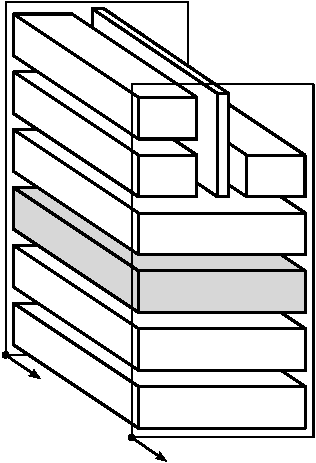
\includegraphics[scale=0.5]{ch3/img/PA_map_obstacle.pdf}
	\begin{tikzpicture}[>=latex',scale=0.4]
	\drawplanexy{-0.3}{-0.3}{-0.3}{6.7}{10}{dashed}{perception}
	
	\drawcube{0}{0}{5}{6.4}{1}{white}{dinamica}{}{};
	\drawcube{0}{1.2}{5}{6.4}{1}{white}{tracking}{}{};
	
	\drawcube{0}{2.4}{5}{6.4}{1}{gray!40}{ostacoli}{}{};
	\drawcube{0}{3.6}{5}{6.4}{1}{white}{altitude}{}{};
	
	\drawcube{0}{4.8}{5}{3}{1.5}{white}{source}{}{};
	\drawcube{0}{6.5}{5}{3}{1.5}{white}{emulatore}{}{};

	\drawplanezy{3.2}{4.8}{5}{4.5}{radar_det}{fill=white,opacity=0.90}{}{};

	\drawcube{3.4}{4.8}{5}{3}{3.2}{white}{alpha}{}{};
	\drawplanexy{-0.3}{-0.3}{5.3}{6.7}{10}{dashed}{action}
	

	\draw [->,line width=1.5] (action_D) -- ++(0,0,2);
	\draw [->,line width=1.5] (perception_D) -- ++(0,0,2);

	\coordinate [at=(radar_det_D), yshift=-5] (arrows_point);
	\draw [->,dashed]  (arrows_point) -- ++(1.5,0,0); 
	\draw [->,dashed]  (arrows_point) -- ++(-1.5,0,0); 
\end{tikzpicture}
\end{marginfigure}
An avalanche has an huge amount of kinetic energy, enough to destroy most of the artificial building and move objects with a big cross--section that are on its traveling path. Thus, the objects that avalanche drone has to avoid are mainly pillars, trees or mounds of snow.

Taken into account this consideration about the surroundings in which the drone will try to find a buried person, it is useless to define an internal map of obstacle and elaborate the optimal trajectory to an ending point because, in fact, for the most of the time the drone will explore without having such a knowledge of the ending point.

This simplification gather different advantage to the final algorithm:
\begin{itemize}
\item we do not need the extremely high computational power needed to maintain such environment projection into agent mind space
\item the obstacle avoidance imposes minor constraints on the upper layer of the searching algorithm, with respect to convoluted algorithm
\item the simplification brings to a more reliable routine, because of its deterministic nature, with respect to a Bayesian based map
\item this algorithm fits technical specification imposed by used hardware
\end{itemize}
while the main drawbacks are
\begin{itemize}
\item we are flying on a non optimal path
\item it is based on a simplification, and real life is always harder than what we aspect
\end{itemize}

Diving into deep, the definition is based upon the presence of one range finder for each arm of the drone. As range finder it is possible to use ultrasonic range finders, that are device that do not have problems on lens like laser ones. An ultrasonic range finder has a characteristic lobe, similar to an antenna directivity lobe, with a peak at almost \num{6}\si{\meter}. 

The algorithm tries to identify a run away speed, given the distance from the obstacle received from each sensor (${d_i\,:\,i=1..6}$):

\begin{equation}
\mathbf{v} = \rotmat \sum\limits_{i=1}^{6}v(d_i)\vettore{\cos\braces{(i-1)\dfrac{\pi}{3}} \\ -\sin\braces{(i-1)\dfrac{\pi}{3}} \\0}
\end{equation}

where ${v(d_i)}$ is a function that defines the velocity magnitude on the direction of the range finder. The first magnitude used was:
\begin{equation}
v(d_i) = - \dfrac{1}{d_i}
\end{equation}
that has some discontinuity problems, so the next function implemented is a sigmoid function:
\begin{equation}
v(d_i) = p_3 \braces{\dfrac{1}{1+e^{4 \braces{\frac{p_1}{2}-d_i}\frac{p_2}{p_3}}}-1}
\end{equation}
\begin{marginfigure}
	\centering
	%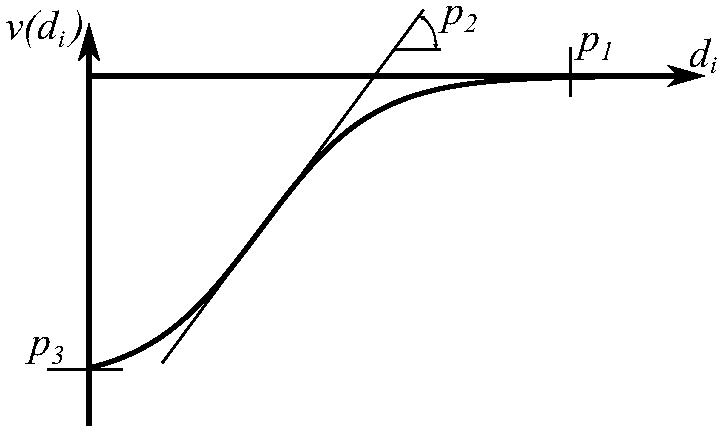
\includegraphics[scale=0.4]{ch3/img/speed_profile.pdf}
	\pgfmathdeclarefunction{speed}{3}{%
		\pgfmathparse{#3 * ( (1)/(1+exp(4*((#1/2)-x)*#2/#3)) - 1 )}%
	}
	\begin{tikzpicture}[>=latex]
		\begin{axis}[
			domain=0:11.5, samples=100,
			enlargelimits=false,
			xmin=0, xmax=12, ymin=-6, ymax=1,
			height=6cm, width=6cm,
			axis lines=middle,
			xlabel=\scriptsize{$d_i$}, ylabel=\scriptsize{$v(d_i)$},
			every axis y label/.style={at=(current axis.above origin),anchor=south },
			every axis x label/.style={at=(current axis.right of origin),anchor=west},
			xtick=\empty, ytick=\empty,
			extra y ticks={-4.7}, extra y tick labels={$p_3$},
			extra x ticks={10}, extra x tick labels={$p_1$}
		]
			\addplot[black,line width=1.5]{speed(7,1,5)};
		\end{axis}
		
		\draw (0.75,1.3) -- ++(240:1) -- ++(60:5) -- ++(240:0.75) -- ++(0.75,0) --++(-0.15,0) coordinate(arco);
		\draw[<->] (arco) arc(0:60:0.6) node [xshift=15] {$p_2$};	
	\end{tikzpicture}
	\caption{Velocity profile}
\end{marginfigure}
from which we obtain a continuous function where the parameters:
\begin{itemize}
\item $p_1$: it is the maximum range, at which considered velocity is zero
\item $p_2$: defines the slope of the curve at ${d_i = p_1/2}$
\item $p_3$: defines the maximum velocity, or the value of the curve for ${d_i = 0}$
\end{itemize}

In figure \ref{fig:obstavoidexample} an example of how the algorithm works is shown. Obviously, signal coming from the algorithm get some sort of filtration to eliminate various source of noise.
\begin{figure}[h]
	\centering
	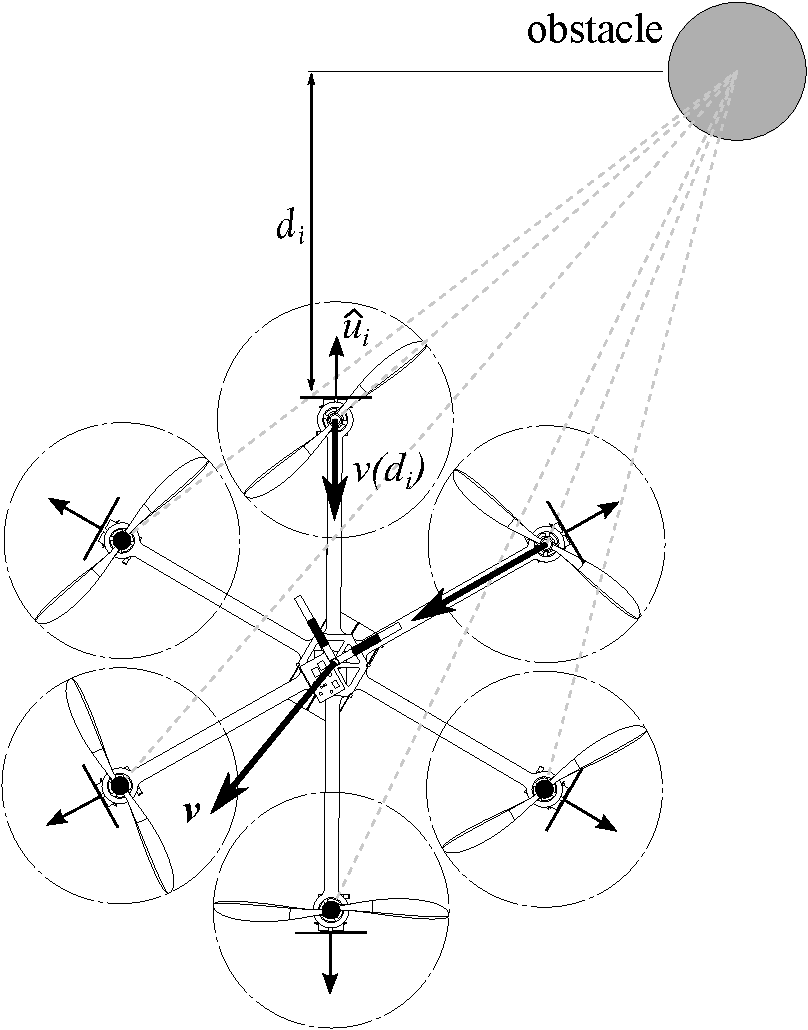
\includegraphics[scale=0.45]{ch3/img/obstavoid_dist.pdf}
	\caption{Example of obstacle avoid algorithm behavior}
	\label{fig:obstavoidexample}
	\forceversofloat
\end{figure}

\myparagraph{Model of range finder}
From the simulation point of view the effects of an obstacle are obtained through a model of the characteristic lobe of each range finder. 
\begin{figure}[h]
	\centering
	%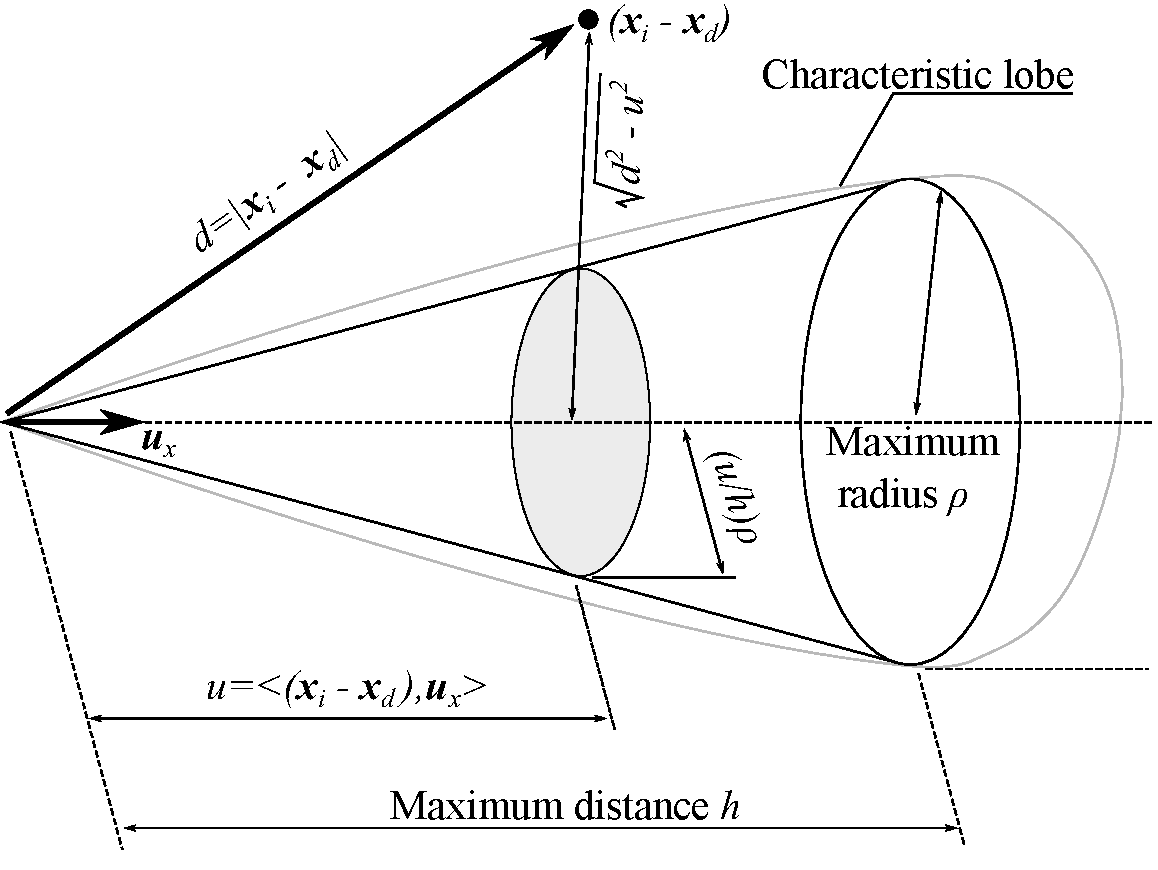
\includegraphics[scale=0.45]{ch3/img/lobe_dimensions.pdf}
	\begin{tikzpicture}[>=latex']
		\draw[dashed,gray] (0,0) .. controls (6cm,3cm) ..  (8.5cm,3.5cm) to[bend left,out=45] (11cm,0cm) to [bend left,in=125] (8.5cm,-3.5cm) .. controls (6cm,-3cm) .. cycle;
	   \draw [fill=gray!40,opacity=40](5cm,0cm) ellipse (0.75cm and 2.05cm);
		\draw (8.5cm,0cm) ellipse (1.25cm and 3.5cm);
		\draw (8.2cm,-3.4cm) -- (0,0) -- (8.2cm,3.4cm);
		\draw[dashed] (0,0) -- (9cm,0);

		\node [circle,inner sep=1pt,fill=black] at (5cm,4cm) {};
		\draw [<->] (5cm,0cm) -- node[pos=0.9,right]{$\sqrt{d_i^2-u^2}$} (5cm,3.9cm);
		\draw [->,line width=1.5] (0cm,0cm) -- (2.5cm,0cm);
		\draw [->,line width=1.5] (0cm,0cm) -- node[above,rotate=38.53]{$d_i = | \mathbf{x}_i^{\Psi} - \mathbf{x}_d|$} (4.9cm,3.9cm);
		\draw [->] (5cm,0cm) -- ++(-70:1.4) node[anchor=west,xshift=3,yshift=-3] {$\dfrac{\rho}{h}u$};
		\node at(4cm,4.3cm) {$(\mathbf{x}_i^{\Psi} - \mathbf{x}_d)$};
		\node at(2.5cm,-0.35cm) {$\hat{\mathbf{u}}_{i}$};

		\draw [->] (8.5cm,0cm) -- ++(-70:2.5) node[anchor=west,xshift=3,yshift=-3] {$\rho$ (maximum radius)};

		\draw (0cm,-0.1cm) -- (0cm,-5cm);
		\draw (4.9cm,-2.2cm) -- (4.9cm,-4cm);
		\draw (8.5cm,-0.1cm) -- (8.5cm,-5cm);
		\draw [<->](0cm,-3.9cm) -- node[pos=0.5,above]{$u=(\mathbf{x}_i^{\Psi} - \mathbf{x}_d) \cdot \hat{\mathbf{u}}_i$} (4.9cm,-3.9cm);
		\draw [<->](0cm,-4.9cm) -- node[pos=0.5,above]{$h$ (maximum range)} (8.5cm,-4.9cm);
		\draw [<-] (9cm,3.5cm) -- ++(45:0.5cm) -- node[pos=0.5,above]{Characteristic lobe} ++(3cm,0); 
	\end{tikzpicture}
	\caption{Range finder algorithm}
	\forcerectofloat
\end{figure}
The obstacles are implemented as sets of points, paradigm that brings a little advantage from the simulation point of view of inserting some noise due to the discontinuities between points, similar to real range finder noise, due to analog to digital conversion.
\begin{equation}
\Psi = \left[ \mathbf{x}_i \,:\,i=1..M  \right]
\end{equation}

For our system we suppose to know exactly the position $\hexastate_d$ and orientation $\rotmat$ of the drone\sidenote{For the obstacle avoidance algorithm only attitude must be know, to project the velocity in ground reference frame}. We define observation versors as follows:
\begin{equation}
\label{eq:versorirangefind}
\left\{ \vers{u}_i \,:\, i=1..6 \right\} \rightarrow \left\{ \vettore{\cos\braces{(i-1)\dfrac{\pi}{3}} \\ -\sin\braces{(i-1)\dfrac{\pi}{3}} \\0} \,:\, i=1..6 \right\}
\end{equation}
The characteristic of the range finder is described with the use of a cone. Distance is evaluated using time of flight of an ultrasonic signal emitted by the oscillator. Mathematically it is possible to define the lobe with a cone in the space, that has axis parallel to the versors defined in \ref{eq:versorirangefind}, and vertex coincident with receiving system. The solid that approximates the characteristic lobe is defined by:
\begin{equation}
\begin{array}{rcl}
x &=& \dfrac{u}{h} \rho \cos(\theta) \\
y &=& \dfrac{u}{h} \rho \sin(\theta) \\
z &=& u
\end{array}
\end{equation}
where the parameters:
\begin{itemize}
\item $h$: receiver maximum distance
\item $\rho$: receiver maximum lobe dimension
\end{itemize}

\begin{algorithm}[h]
\label{alg:rangefinder}
\caption{Range finder points}
\SetKw{KwAs}{as}
\KwData{$h,\,\rho$}
\ForEach{Obstacle \KwAs $\Psi$}{
	\tcc{Exec for each point of an obstacle}
	\For{$i=1$ \KwTo $M$}{ 
		${\mathbf{d}_i^{\Psi} \leftarrow \mathcal{R}^T(\phi,\theta,\psi) \braces{\mathbf{x}_{i,\mathrm{ground}}^{\Psi}-\mathbf{x}_d}}$\;
		\For{$j=0$ \KwTo 5}{
			${D_{i,j}^{\Psi} \leftarrow \mathbf{d}_i^{\Psi} \cdot \vers{u}(j\pi/3)}$\;
			\tcc{Check if the point is in cone, else distance is $\infty$}
			\eIf{$\braces{0\leq D_{i,j}^{\Psi} \leq h}$}{
				\If{$\braces{\mathbf{d}_i^{\Psi} \cdot \mathbf{d}_i^{\Psi} - {D_{i,j}^{\Psi}}^2 \geq \braces{\dfrac{\rho}{h} D_{i,j}^{\Psi}}^2 }$}{
					${D_{i,j}^{\Psi} \leftarrow \infty}$\;
				}
			}{
				${D_{i,j}^{\Psi} \leftarrow \infty}$ \;
			}
		}
	}
}
\tcc{Search minimum distance for each sensor}
$\mathbf{r} \leftarrow [r_j = \infty\,:\,j=0$ \KwTo $5]$\;
\For{$j=0$ \KwTo 5}{
	\ForEach{Obstacle \KwAs $\Psi$}{
		\For{$i=1$ \KwTo $M$}{
			\If{$r_j \geq D_{i,j}^{\Psi}$}{
				$r_j \leftarrow D_{i,j}^{\Psi}$ \;
			}
		}
	}
}
\Return{$\mathbf{r}$}
\end{algorithm}

Given a point ${\mathbf{x}_i \in \Psi}$, if it is inside the cone, the projection of the distance ${\mathbf{x}_d-\mathbf{x}_i}$ on the axis of the cone is the identified distance.

The algorithm describes how each sensor returns the minimum identified distance that is inside its cone. The distances are used to build the velocity vector that avoid the obstacle.

\FloatBarrier
\section{Altitude keeping}
\begin{marginfigure}
	\centering
	%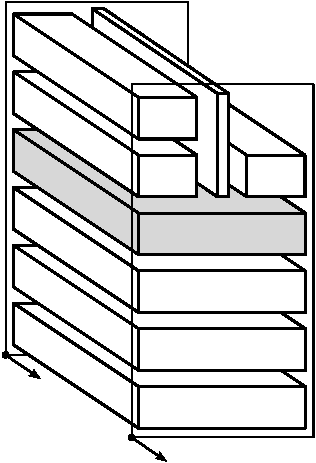
\includegraphics[scale=0.5]{ch3/img/PA_map_altitude.pdf}
	\begin{tikzpicture}[>=latex',scale=0.4]
	\drawplanexy{-0.3}{-0.3}{-0.3}{6.7}{10}{dashed}{perception}
	
	\drawcube{0}{0}{5}{6.4}{1}{white}{dinamica}{}{};
	\drawcube{0}{1.2}{5}{6.4}{1}{white}{tracking}{}{};
	
	\drawcube{0}{2.4}{5}{6.4}{1}{white}{ostacoli}{}{};
	\drawcube{0}{3.6}{5}{6.4}{1}{gray!40}{altitude}{}{};
	
	\drawcube{0}{4.8}{5}{3}{1.5}{white}{source}{}{};
	\drawcube{0}{6.5}{5}{3}{1.5}{white}{emulatore}{}{};

	\drawplanezy{3.2}{4.8}{5}{4.5}{radar_det}{fill=white,opacity=0.90}{}{};

	\drawcube{3.4}{4.8}{5}{3}{3.2}{white}{alpha}{}{};
	\drawplanexy{-0.3}{-0.3}{5.3}{6.7}{10}{dashed}{action}
	

	\draw [->,line width=1.5] (action_D) -- ++(0,0,2);
	\draw [->,line width=1.5] (perception_D) -- ++(0,0,2);

	\coordinate [at=(radar_det_D), yshift=-5] (arrows_point);
	\draw [->,dashed]  (arrows_point) -- ++(1.5,0,0); 
	\draw [->,dashed]  (arrows_point) -- ++(-1.5,0,0); 
\end{tikzpicture}
\end{marginfigure}
The last basic block that should be implemented is the altitude keeping, to maintain the distance of the drone to the soil high enough to avoid contact with rescuer and low enough to get a good signal strength. The sensors used are, again, ultrasonic range finder. With respect to the obstacle avoidance, that acts as a control on the lateral dynamic of the drone, that is quite slow, altitude keeping works on vertical dynamic that is really fast, and need a more reliable implementation, and require a statistical system to determine the distance even with a high irregular terrain.

This part was actually not implemented because of the need of more test about response of ultrasonic waves upon snow surface, to better understand the effects of density on perceived distance.

\subsection{Kalman Filter}
We assume that the dimension could be described with the use of normal distribution:
\begin{equation}
p(\hexastate) \det\braces{(2\pi)^{n}\Sigma_0}^{-1/2} e^{-\dfrac{1}{2}\braces{\hexastate - \boldsymbol{\mu}}^T \Sigma^{-1}\braces{\hexastate - \boldsymbol{\mu}}}
\end{equation}
with ${\boldsymbol{\mu}}$ the mean value for the distribution and ${\Sigma}$ covariance matrix of the distribution.

The Kalman filter include the knowledge of the covariance matrix into the state estimation procedure, and it is possible to proof that the final estimation will maintain a normal distribution if:
\begin{itemize}
\item distribution of initial state is normal
\item the state distribution is a linear function of the previous state and a white Gaussian noise
\item the measurement distribution  is a linear function of the state and a white Gaussian noise
\end{itemize}

\myparagraph{Initial state probability}
We make the really strong hypothesis to have an initial distribution in the normal form:
\begin{equation}
p(\hexastate_0) \det\braces{(2\pi)^{n}\Sigma_0}^{-1/2} e^{-\dfrac{1}{2}\braces{\hexastate_0 - \boldsymbol{\mu_0}}^T \Sigma_{0}^{-1}\braces{\hexastate_0 - \boldsymbol{\mu_0}}}
\end{equation}

\myparagraph{Prediction phase}
The distribution of the state derives from the distribution of the previous state, using the linear relation:
\begin{equation}
\hexastate_t = A_t \hexastate_{t-1} + B \hexacontrol_t + \statenoise
\end{equation}
where ${\mathbf{w}_t}$ is a realization of a distribution ${\mathcal{N}(\mathbf{0},R_t)}$ in which $R_t$ is the matrix that describes the covariance of the noise on the state.

The distribution is normal due to the relations:
\arraymath{
\bar{\boldsymbol{\mu}_{t}} &=& A_t \boldsymbol{\mu}_{t-1} + B_t \hexacontrol_{t} \\
\bar{\Sigma_{t}} &=& A_t \Sigma_{t-1} A_t^T + R_t \\
p(\hexastate_t \mid \hexastate_{t-1}, \hexacontrol_t) &=& \det((2\pi)^n R_t)^{-\frac{1}{2}} e^{\left( - \frac{1}{2} (\hexastate_t - \bar{\boldsymbol{\mu}_{t}})^T {R_t}^{-1} (\hexastate_t - \bar{\boldsymbol{\mu}_{t}}) \right)}
}

If the system has a non--linear function that describes the dynamic, it could be approximated with a first--order Taylor expansion:
\begin{equation}
\hexastate_t = g\braces{\hexastate_{t-1},\hexacontrol_t} + \statenoise
\end{equation}
\arraymath{
\mathrm{Taylor}_{1}\left(g(\hexastate_{t-1},\hexacontrol_t)\right)\Big\rfloor_{\bar{\boldsymbol{\mu}}_{t-1},\bar{\hexacontrol}_t} & = & g(\bar{\boldsymbol{\mu}}_{t-1},\bar{\hexacontrol}_t) + \\ & & \nabla_{\hexastate} g (\hexastate_{t-1},\hexacontrol_t)\Big\rfloor_{\bar{\boldsymbol{\mu}}_{t-1},\bar{\hexacontrol}_t}\left( {\hexastate}_{t-1} - \bar{\boldsymbol{\mu}}_{t-1} \right) \\
& = & g(\bar{\boldsymbol{\mu}}_{t-1},\bar{\hexacontrol}_t) + A_t\left( {\hexastate}_{t-1} - \bar{\boldsymbol{\mu}}_{t-1} \right)
}

\myparagraph{Estimation state}
The measurement distribution derives directly from the measurement model:
\begin{equation}
\mathbf{z}_t = C_t \hexastate_t + \measnoise
\end{equation}
where ${\mathbf{v}_t}$ is a realization of a distribution ${\mathcal{N}(\mathbf{0},Q_t)}$ in which $Q_t$ is the matrix that describes the covariance of the noise on the measurement.

The distribution maintains its normal behavior due to the relation:
\[p(\mathbf{z}_t\mid\hexastate_t) = \det((2\pi)^n Q_t)^{-\frac{1}{2}} e^{\left( -\frac{1}{2} (\mathbf{z}_t - C_t \hexastate_t)^T Q_t^{-1} (\mathbf{z}_t - C_t \hexastate_t) \right)}\]

If the measurement is modeled with the use of a non--linear function it is possible to use a Taylor expansion to approximate locally the measurement function:
\begin{equation}
\mathbf{z}_t = h(\hexastate_t) + \measnoise
\end{equation}
\arraymath{
\mathrm{Taylor}_{1}\left(h(\hexastate_{t})\right)\Big\rfloor_{\bar{\boldsymbol{\mu}}_{t}} & = & h(\bar{\boldsymbol{\mu}}_{t}) + \nabla_{\hexastate} h (\hexastate_{t})\Big\rfloor_{\bar{\boldsymbol{\mu}}_{t-1}}\left( {\hexastate}_{t} - \bar{\boldsymbol{\mu}}_{t} \right) \\
 & = & h(\bar{\boldsymbol{\mu}}_{t}) + C_t\left( {\hexastate}_{t} - \bar{\boldsymbol{\mu}}_{t} \right)
}

\myparagraph{Complete KF algorithm}
Now we are ready to define a complete Kalman Filter. The blue lines represent the step that should be performed in the case of non--linear models. Must be noticed, that in case of such non--linearities, it is impossible to demonstrate the fact that normal posterior distribution are maintained.
\begin{algorithm}[h]
\caption{(Extended) Kalman Filter}
\KwData{$\stateest_{t-1},\,\statecovest_{t-1},\,\hexacontrol_t,\,\measset_t$}
\tcc{Prediction phase}
\eIf{Model is linear}{
	${\statepred_t = A_t \stateest_{t-1} + B_t \hexacontrol_t}$ \;
	${\measpred_t = C_t \statepred_t}$ \;
}{
	${\color{blue} \statepred_t = g\braces{\stateest_{t-1},\hexacontrol_t}}$ \;
	${\color{blue} A_t = \nabla_{\hexastate}g\braces{\hexastate_{t-1},\hexacontrol_t} \Big\rfloor_{\statepred_{t-1},\hexacontrol_t}}$ \;
	${\color{blue} B_t = \nabla_{\hexastate}h\braces{\hexastate_{t-1}} \Big\rfloor_{\statepred_{t-1},\hexacontrol_t}}$ \;
	${\color{blue} \measpred_t = h(\statepred_t)}$ \;
}
${\statecovpred_t = A_t \statecovpred_{t-1} A_t + \statecovnoise}$ \;
\tcc{Evaluation of Kalman Gain}
${\kfgain = \statecovpred_t C_t^T \braces{ C_t \statecovpred_t C_t^T + \meascovnoise }^{-1}}$ \;
\tcc{Estimation phase}
${\stateest_t = \statepred_t + \kfgain \braces{\measset_t - \measpred_t}}$ \;
${\statecovest_t = \braces{\mathbb{I} - \kfgain C_t} \statecovpred_t}$ \;
\Return{${\stateest_t,\,\statecovest_t}$}
\end{algorithm}
\FloatBarrier
\subsection{Application to altitude keeping}
\begin{figure}[h]
	\centering
	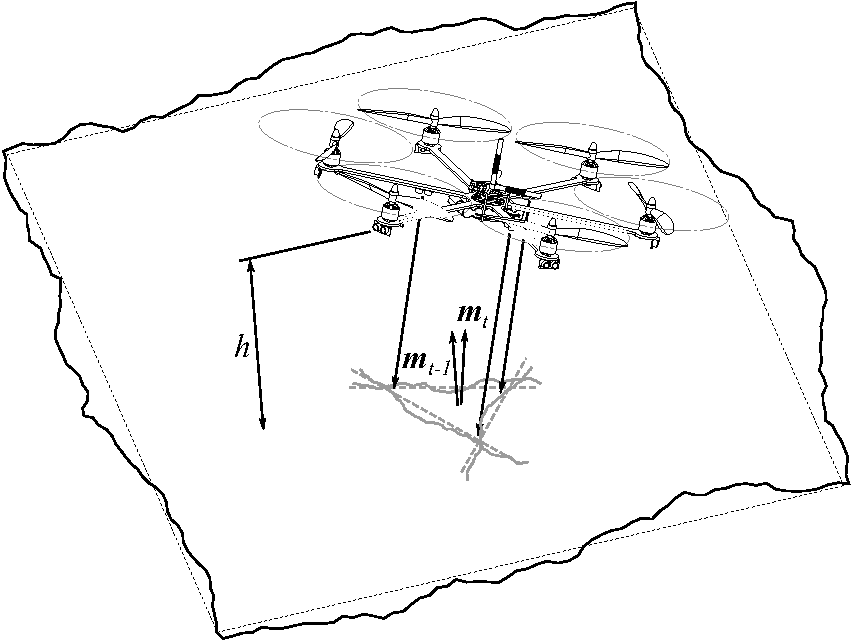
\includegraphics[scale=0.65]{ch3/img/altitude_keep.pdf}
	\caption{Altitude keeping problem}
	\forceversofloat
\end{figure}
\FloatBarrier
We can model the problem taking into account attitude dynamic and vertical dynamic of the VTOL, from which we know also the rotation matrix of the drone. The plane of the avalanche could be approximated through the orthogonal versor $\vers{m}$, projected in the drone reference frame. The problem, inserting $\vers{m}$ into the state vector, becomes equivalent to a \emph{SLAM}\sidenote[][-1cm]{\emph{SLAM}: Simultaneous Localization And Mapping} problem.

The state is:
\renewcommand{\arraystretch}{1}
\begin{equation}
\hexastate = \vettore{\hexastate \\ \vers{m}_b}
\end{equation}
\renewcommand{\arraystretch}{1.75}
and the covariance matrix of the state derives from covariance of the position system at which must be added a covarianc ematrix on the knowledge of ${\vers{m}_b = \rotmat^{T} \vers{m}}$. We could use three range finder directed to the ground, under the drone, that allow us to define three points on the surface. A model for the measurement function uses some simple algebraic definitions: given three points that belong to the plane, $\{A,\, B,\, C\}$, the normal is:
\begin{equation}
\vers{m} = \dfrac{(A-B)\times(B-C)}{\abs{(A-B)\times(B-C)}}
\end{equation}

Once normal is know, it could be used to implement a tracking control that maintains a certain distance on the normal vector. As already said, the performance of this algorithm depends directly from the estimation of the covariance matrix for measurement, and upon the sonar response due to variation of snow on the field.
%\FloatBarrier7
\section{The signal detection problem}
\begin{marginfigure}
	\centering
	%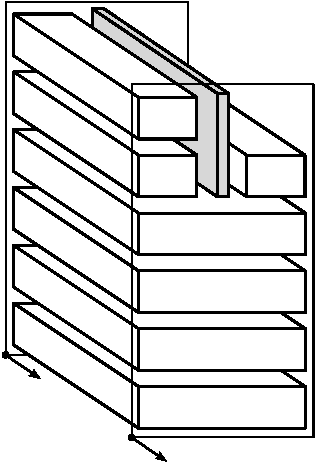
\includegraphics[scale=0.5]{ch3/img/PA_map_radar.pdf}
	\begin{tikzpicture}[>=latex',scale=0.4]
	\drawplanexy{-0.3}{-0.3}{-0.3}{6.7}{10}{dashed}{perception}
	
	\drawcube{0}{0}{5}{6.4}{1}{white}{dinamica}{}{};
	\drawcube{0}{1.2}{5}{6.4}{1}{white}{tracking}{}{};
	
	\drawcube{0}{2.4}{5}{6.4}{1}{white}{ostacoli}{}{};
	\drawcube{0}{3.6}{5}{6.4}{1}{white}{altitude}{}{};
	
	\drawcube{0}{4.8}{5}{3}{1.5}{white}{source}{}{};
	\drawcube{0}{6.5}{5}{3}{1.5}{white}{emulatore}{}{};

	\drawplanezy{3.2}{4.8}{5}{4.5}{radar_det}{fill=gray!40,opacity=0.90}{}{};

	\drawcube{3.4}{4.8}{5}{3}{3.2}{white}{alpha}{}{};
	\drawplanexy{-0.3}{-0.3}{5.3}{6.7}{10}{dashed}{action}
	

	\draw [->,line width=1.5] (action_D) -- ++(0,0,2);
	\draw [->,line width=1.5] (perception_D) -- ++(0,0,2);

	\coordinate [at=(radar_det_D), yshift=-5] (arrows_point);
	\draw [->,dashed]  (arrows_point) -- ++(1.5,0,0); 
	\draw [->,dashed]  (arrows_point) -- ++(-1.5,0,0); 
\end{tikzpicture}
\end{marginfigure}
We have two searching status for our agent. In one searching status, the VTOL tries to identify a signal, while in the second stage, once we have identified the presence of a signal, the drone has to find the transmission source point. The passage from a searching strategy to another is the\emph{supervised signal detection}.

\subsection{Supervised signal detection}
What we are trying to define is a strategy that is able to detect a target signal from a background noise. This is not new to signal theory, if we look at radar research work.
\begin{marginfigure}
	\centering
	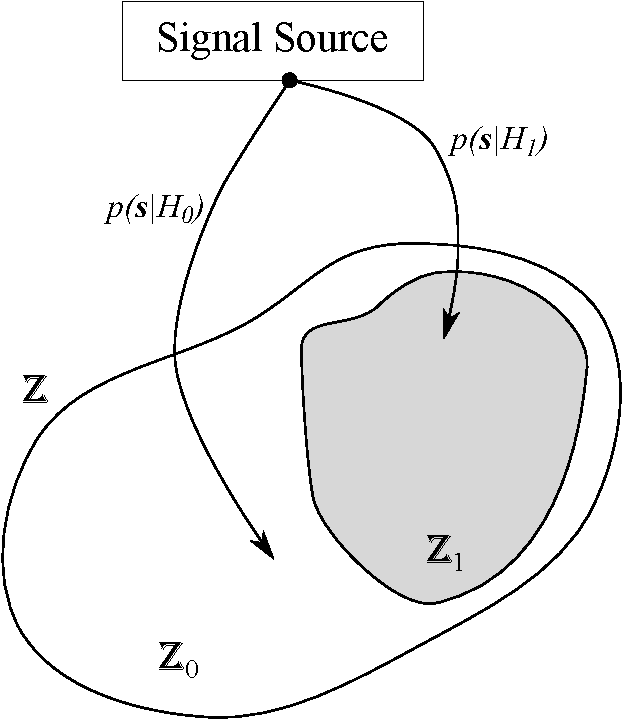
\includegraphics[scale=0.5]{ch3/img/signalsources.pdf}
	\caption{Decision spaces}
\end{marginfigure}
The detection theory is seen as a binary classification problem based upon two hypothesis:
\begin{itemize}
\item hypothesis $0$: absence of signal
\item hypothesis $1$: presence of signal
\end{itemize}
The choice is made upon a signal ${\signal = [s_1,\dots,s_n]}$ in which a certain number of feature identifies its belonging to a decision field or observation space $\decspace \in \mathbb{R}^n$. The observation space is defined by the union of two decision regions:
\[ \decspace \equiv \decspacezero \cup \decspaceone \]
Each decision space has a conditional \emph{PDF}, that is assumed to be known:
\arraymath{
	\decspacezero & \mapsto & p(\signal|\hypzero) \\
	\decspaceone & \mapsto & p(\signal|\hypone) \\
}

\subsection{Risk criterion}
The classification is based upon criteria, such as:
\begin{itemize}
\item Minimum Risk Criterion
\item Minimax Criterion
\item Neyman--Pearson Criterion
\end{itemize}
That represents the classification strategies.

\myparagraph{Minimum risk criterion}
This criterion is based upon the assumptions that posteriors probability ${P(\hypzero|\signal)}$ and ${P(\hypone|\signal)}$ are known, and also the cost matrix is known, where the matrix is defined in table \ref{tbl:cost_matrix}.
\begin{margintable}
	\renewcommand{\arraystretch}{1}
	\begin{centering} 
		\begin{tabular}{>{\centering} m{1.25cm} <{\centering} | >{\centering} m{1.25cm} <{\centering} >{\centering} m{1.25cm} <{\centering}}
		\hline										& \scriptsize{\textbf{Decide absent}\newline$D_0$} & \scriptsize{\textbf{Decide present}\newline$D_1$} \tabularnewline \hline
		\scriptsize{\textbf{Signal absent}\newline$\hypzero$}  	& \cellcolor{lgray}\scriptsize{Correct rejection:\newline$c_{0,0}$} & \cellcolor{dgray}\scriptsize{False alarm:\newline$c_{1,0}$}        \tabularnewline
		\scriptsize{\textbf{Signal present}\newline$\hypone$} 	& \cellcolor{dgray}\scriptsize{Miss:\newline$c_{0,1}$}              & \cellcolor{lgray}\scriptsize{Hit:\newline$c_{1,1}$}                \tabularnewline \hline
		\end{tabular}
	\end{centering} 
	\renewcommand{\arraystretch}{1.75}
	\caption{Costs matrix}
	\label{tbl:cost_matrix}
\end{margintable}
In practice we have: ${c_{0,1} > c_{1,1}}$ and ${c_{1,0} > c_{0,0}}$.

The main objective is to \emph{minimize the average cost incurred by erroneous decision}\TODO{citep libro pattrec}. This is done through a minimization of a risk function defined over observation space. This optimization allows us to define the decision regions $\decspacezero$ and $\decspaceone$ which are optimal in terminal of overall risk. We define the risk:
\begin{equation}
R = c_{0,0} P(D_0, \hypzero) + c_{1,0} P(D_1, \hypzero) + c_{0,1} P(D_0, \hypone) + c_{1,1} P(D_1, \hypone)
\end{equation}
using the axiom of probability on $P(D_i,H_j)$, we get in general:
\begin{equation}
P(D_i,H_j) = P(D_i|H_j) P(H_j) \qquad (i,j) \in (0..1,0..1)
\end{equation}
and also:
\begin{equation}
P(D_i|H_j) = \int\limits_{\decspace_i}P(\signal|H_j)d\signal
\end{equation}
The evaluation, for each conditional probability is:
\begin{marginfigure}
	\centering
	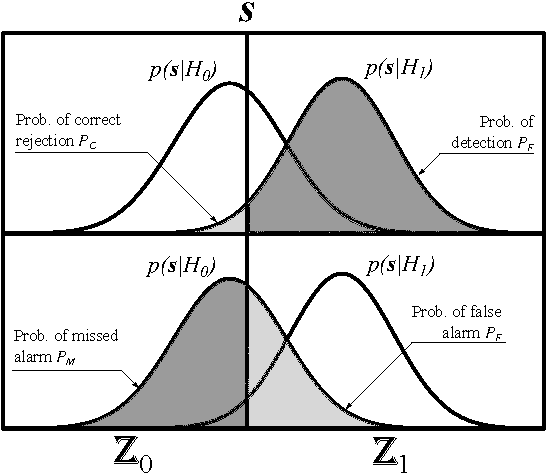
\includegraphics[scale=0.55]{ch3/img/probcurves.pdf}
	\caption{Probability versus decision space}
\end{marginfigure}
\arraymath{
	P(D_0|\hypzero) & = & \int\limits_{\decspacezero}p(\signal|\hypzero)d\signal = 1 - \probfalse \\
	P(D_0|\hypone) & = & \int\limits_{\decspacezero}p(\signal|\hypone)d\signal = \probmiss \\
	P(D_1|\hypzero) & = & \int\limits_{\decspaceone}p(\signal|\hypzero)d\signal = \probfalse \\
	P(D_1|\hypone) & = & \int\limits_{\decspaceone}p(\signal|\hypone)d\signal = 1 - \probmiss
}
where:
\begin{itemize}
\item $\probrej$: represents probability of correct rejection
\item $\probfalse$: represents probability of false alarm
\item $\probmiss$: represents probability of missed alarm
\item $\probdet$: represents probability of detection
\end{itemize}
and, looking at figure \ref{fig:probdetection}, stands the relation:
\arraymath{
	\probdet + \probmiss & = & 1 \\
	\probrej + \probfalse & = & 1
}

Finally, we get the defintion of risk:
\begin{equation}
\begin{array}{rcl} 
R & = & c_{0,0} \braces{1-\probfalse} P(\hypzero) + c_{0,1} \probmiss P(\hypone) + \\ 
  &   &  + c_{1,0} \probfalse P(\hypzero) + c_{1,1} (1-\probmiss) P(\hypone) \\
  & = & P(\hypzero) \braces{c_{0,0} + \probfalse (c_{1,0} - c_{0,0})} + P(\hypone) \braces{c_{1,1} + \probmiss (c_{0,1} - c_{1,1})}
\end{array}
\end{equation}
applying some substitutions:
\arraymath{
	\probmiss & = & \int\limits_{\decspacezero}p(\signal|\hypone)d\signal \\
	\probfalse & = & \int\limits_{\decspaceone}p(\signal|\hypzero)d\signal =  \\
	    & = & 1 - \int\limits_{\decspacezero}p(\signal|\hypzero)d\signal  \\
	1 & = & \int\limits_{\decspacezero}p(\signal|H_j)d\signal + \int\limits_{\decspaceone}p(\signal|H_j)d\signal 
}
and the risk equation:
\begin{equation}
\begin{array}{rcl}
R & = & P(\hypzero) \braces{c_{0,0} + \probfalse (c_{1,0} - c_{0,0})} + P(\hypone) \braces{c_{1,1} + \probmiss (c_{0,1} - c_{1,1})} = \\ 
  & = & P(\hypzero) \braces{c_{0,0} + \braces{1 - \int\limits_{\decspacezero}p(\signal|\hypzero)d\signal} (c_{1,0} - c_{0,0})} + \\ 
  &   &  + P(\hypone) \braces{c_{1,1} + \braces{\int\limits_{\decspacezero}p(\signal|\hypone)d\signal} (c_{0,1} - c_{1,1})} = \\ 
  & = & P(\hypzero) c_{1,0} + P(\hypone) c_{1,1} + \\
  &   & + \int\limits_{\decspacezero} P(\hypone)\braces{c_{0,1} - c_{1,1}} p(\signal|\hypone) - P(\hypzero)\braces{c_{1,0} - c_{0,0}} p(\signal|\hypzero) d\signal
\end{array}
\end{equation}
The first part is constant, to minimize the risk we have to work on the argument of the integral, that depends upon ${\decspacezero}$. Because:
\arraymath{
	P(\hypone)\braces{c_{0,1} - c_{1,1}} p(\signal|\hypone) & \geq & 0 \\
	P(\hypzero)\braces{c_{1,0} - c_{0,0}} p(\signal|\hypzero) & \geq & 0
}
the risk is minimized when:
\begin{equation}
P(\hypone)\braces{c_{0,1} - c_{1,1}} p(\signal|\hypone) < P(\hypzero)\braces{c_{1,0} - c_{0,0}} p(\signal|\hypzero)
\end{equation}
and rearranged as follow
\begin{equation}
\naming{ \dfrac{p(\signal|\hypone)}{p(\signal|\hypzero)} }{\likelihood} < \naming{ \dfrac{P(\hypzero)\braces{c_{1,0} - c_{0,0}}}{P(\hypone)\braces{c_{0,1} - c_{1,1}}} }{\threshold}
\end{equation}
that allow us to define the algorithm \ref{alg:minimumrisk}. Must be noticed:
\begin{itemize}
\item because of the binary nature, the decision rule obtained with the minimization on a single decision, grant the minimization of the risk also on the other decision; thus we could say that the local decision rule minimizes the overall risk
\item the likelihood ratio and threshold define decision regions as follows:
\arraymath{
	\decspacezero &=& \{ \signal\in\decspace \,:\,\likelihood<\threshold \} \\
	\decspaceone &=& \{ \signal\in\decspace \,:\,\likelihood>\threshold \} 
}
and a sample such that $\likelihood=\threshold$ could be assigned arbitrarily to one of the decision region
\item the distributions ${p(\signal|\hypzero)}$ and ${p(\signal|\hypone)}$ should be derived experimentally, something that is not to difficult because of characteristics of our signal
\end{itemize}
\begin{algorithm}[h]
\caption{Minimum risk criterion}
\label{alg:minimumrisk}
\KwData{ $p(\signal|\hypone),\,p(\signal|\hypzero),\,c_{0,0},\,c_{1,0},\,c_{0,1},\,c_{1,1}$ }
\tcc{Define the likelihood ratio}
$\likelihood \leftarrow \dfrac{p(\signal|\hypone)}{p(\signal|\hypzero)} $ \;
\tcc{Define the threshold}
$\threshold \leftarrow \dfrac{P(\hypzero)\braces{c_{1,0} - c_{0,0}}}{P(\hypone)\braces{c_{0,1} - c_{1,1}}}$ \;
\tcc{Binary classification}
\ForAll{$\signal_{in}$}{
	\eIf{$\Lambda(\signal_{in}) \leq \threshold$}{
		\Return{$\signal \in \hypzero$}
	}{
		\Return{$\signal \in \hypone$}
	}
}
\end{algorithm}

\myparagraph{The feature space}
The feature space that could be used are the three signal received from the three orthogonal antennas, plus the position. Te insertion of the position in the feature space is not important for the actual implementation, but could be useful in future, if some computer vision algorithm will be implemented. Algorithms that are able to represent symbolically the dimensions of the avalanche front, in conjunction with slope of the avalanche obtained by the altitude keeping routine, may allow us to define a probability distribution of the possible buried victims, distribution that could be inserted as a priori knowledge in radar detection and searching algorithm.
\FloatBarrier
\section{Searching for the signal}
\begin{marginfigure}
	\centering
	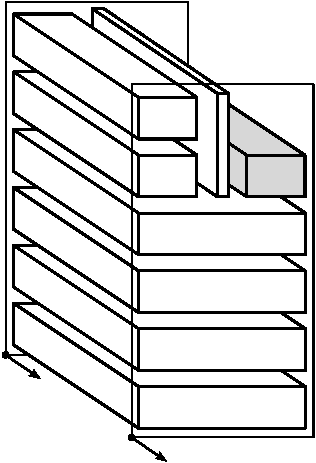
\includegraphics[scale=0.5]{ch3/img/PA_map_exploration.pdf}
\end{marginfigure}
In this section we derive a very simple method to cover the avalanche front to search for a signal beacon. The algorithm presented is incredibly simple and derives from what is actually done by a rescuer on the avalanche front. We try to cover the area of the avalanche with straight equi--spaced lines generated from a series of points.
\begin{figure*}[p]
\caption{Exploration algorithm} \label{fig:exploration} \centering
\begin{tikzpicture}[auto,node distance=0.5cm and 1cm, >=latex', minimum width=3cm, minimum height=1cm, text width=4cm, align=center]

	%\draw (0,0) ellipse (2cm and 1cm) node (start) {Start};
	%\draw

	\node [ellipse, draw, minimum width=2cm, text width=2cm, fill=gray!40] (start) {Start};
	\node [trapezium, draw, trapezium left angle=70,trapezium right angle=-70, below=of start] (inserimento) {Receiving starting point $\mathbf{p}_0$, ending point $\mathbf{p}_n$, plane direction};
	\node [rectangle, draw, below=of inserimento] (generazione_punti) {Generation of points vector $\mathbf{P} = [\mathbf{p}_0,\dots,\mathbf{p}_n]$, set confidence distance $\Delta$};
	\node [rectangle, draw, below=of generazione_punti] (abilita_ricerca) {Start searching sensors, start radar detection routines $\Lambda(\mathbf{s}) \overset{?}{<>} \eta$ };
	\node [rectangle, draw, below=of abilita_ricerca] (goto_start) {$i \leftarrow 0$};
	\node [rectangle, draw, below=of goto_start, text width=2cm] (select_point) {Go To $\textbf{p}_i$};
	\node [trapezium, draw, trapezium left angle=70, trapezium right angle=-70, below=of select_point,text width=1.2cm] (read_position) {Get $\mathbf{x}$};
	\node [diamond, draw, aspect=2, text width=2.3cm, below=of read_position] (distanza) {$\left| \mathbf{p}_i - \mathbf{x} \right| < \Delta$ ?};
	\node [diamond, draw, aspect=2, text width=2cm, below=of distanza] (lastpoint) {$i = n$ ?};
	\node [ellipse, draw, minimum width=2cm, text width=2cm, below=of lastpoint,fill=gray!40] (stop) {Stop};

	\node [rectangle,draw,left=of lastpoint, text width=1.5cm] (addone) { $i \leftarrow i+1$ };
	\coordinate [at=(select_point.north), shift=(0:22mm)] (braces_a);
	\coordinate [at=(distanza.south), shift=(0:22mm)] (braces_b);
	\draw [decorate,decoration={brace,amplitude=12pt}] (braces_a) -- (braces_b) {};

	\node [diamond, draw, aspect=2, text width=2cm, at=(read_position.north east), shift=(0:50mm)] (detection) {$\Lambda(\mathbf{s}) > \eta$?};
	\node [rectangle, draw,fill=gray!40, text width=2.5cm, below=of detection] (search) {Search \mbox{H--field} source};

	\coordinate [at=(detection.north), shift=(90:5mm)] (extraA);
	\coordinate [at=(search.south), shift=(270:5mm)] (extraB);
	\coordinate [at=(detection.west), shift=(180:5mm)] (extraC);
	\coordinate [at=(distanza.west), shift=(180:10mm)] (intraB);

	\draw [->] (start) -- (inserimento);
	\draw [->] (inserimento) -- (generazione_punti);
	\draw [->] (generazione_punti) -- (abilita_ricerca);
	\draw [->] (abilita_ricerca) -- (goto_start);
	\draw [->] (goto_start) -- coordinate[pos=0.5](intraA) (select_point);
	\draw [->] (select_point) -- (read_position);
	\draw [->] (read_position) -- (distanza);
	\draw [->] (distanza) -- node[shift=(0:-17mm)]{\scriptsize{true}} (lastpoint);
	\draw [->] (lastpoint) -- node[shift=(0:-17mm)]{\scriptsize{true}} (stop);
	\draw [->] (detection) -- node[shift=(0:-17mm)]{\scriptsize{true}} (search);
	\draw [->] (lastpoint) -- node[shift=(45:3mm)]{\scriptsize{false}} (addone);

	\draw [->,dashed] (extraA) -- (detection);
	\draw [->,dashed] (search) -- (extraB);
	\draw [->,dashed] (detection) -- node[shift=(45:3mm)]{\scriptsize{false}} (extraC);

	\draw [->] (addone) |- (intraA);
	\draw (distanza) -- node[shift=(45:3mm)]{\scriptsize{false}} (intraB) |- (intraA);

\end{tikzpicture}
\end{figure*}

When turned on, the drone require insertion of two GPS coordinates, or  and a direction from the rescuer. Those two coordinates represent starting point and ending point for the first level of search. Those two points defines a rectangle, the direction represent the orientation of the rectangle. Those data could be inserted from a media device such as tablet or smarthphone.

Once the search area is defined, it is divided into a regular grid, identified by points in the center of each square of the grid. Due to the fact that such input derives from an external device that has computational power, we could use this external device to perform such calculation.

Once the points array is defined, drone simply uses the lower levels of the map to reach each point in sequence. In some cases may be impossible to reach the specific point, due to causes like obstacle or uncertainty due to the motion. To avoid this problem, for each point, is associated a confidence distance, that defines a sphere in which the drone should fly before going to the next point. When last point is reached mission is over. A flowchart of algorithm is presented in figure \ref{fig:exploration}.

\TODO{Immagine esplicativa}

\section{Source searching algorithm}

Some new papers in searching suggested the use of a modified version of the \emph{SLAM} problem to identify position of the source and direction of the dipole. Even if some promising results are exposed in cited papers \citep{pinies2006fast,pinies2006localization}, we were not able to reproduce such results with our system in simulations; because of that, we decided to drop this approach to use one that fit better the perception--action paradigm.

The proposed algorithm uses a two component algorithm.

\subsection{Exploration step}
\begin{marginfigure}
	\centering
	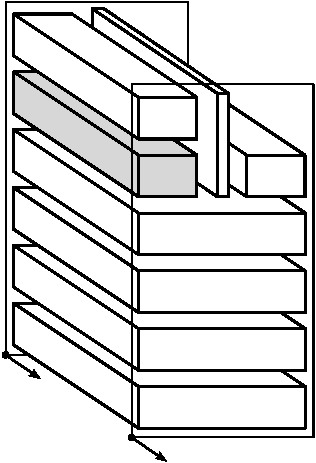
\includegraphics[scale=0.5]{ch3/img/PA_map_direction.pdf}
\end{marginfigure}
The first step is simply an adaptive filter, stolen from the evaluation of Round--Trip--Time in TCP networking, that tries to identify a direction in which the signal is maximized, given an adapted previous knowledge. The algorithm takes into consideration the presence of fluctuations due to noise and interference and changes orientation only when the change in signal is obvious. Scaling parameter regulate the velocity that will move the drone.

An adaptive filter for a variable $x$ is defined as:
\[
x_k = \alpha x_{k-1} + (1-\alpha) \hat{x}_k \qquad 0 \leq \alpha \leq 1
\]

The first part is a mean sampler, that helps us to partially eliminate the white Gaussian noise:
\begin{equation}
	\hat{\hfield}_g = \dfrac{1}{N} \rotmat \sum\limits_{i=0}^{N} \hfield_{b,i}
\end{equation}
Starting from the vector of received signal $\hfield$, the value measured is a vector in hexa--copter body reference frame, and should be reported in ground reference frame, using the state of the drone. From the projection of the H--field some information are extracted, like \textbf{intensity} and \textbf{direction on} $(\vrx\times\vry)$ \textbf{plane}:
\begin{equation}
\begin{array}{rcl}
	\ccos{\alpha} & = & \ccos{\arctan_2(H_y,H_x)} \\
	\ssin{\alpha} & = & \ssin{\arctan_2(H_y,H_x)} \\
	\abs{\hfield} & = & \sqrt{H_x+H_y+H_z}
\end{array}
\end{equation}
The next step is a filtering to eliminates some of the residual noise, with a second order filter. We exploit the discontinuity problem of the ${\arctan_2(\cdot)}$ function using trigonometric functions. From the input values:
\begin{itemize}
\item the value of the measured field is used to steer the system in direction of the source, to avoid symmetric problem of the received field
\item the adapted H--field measurement defines the speed, throug a function ${v(\cdot)}$
\item the direction of speed is defined using adapted angle
\end{itemize}
The effect of this routine is only to explore the environment in a direction the maximizes the received signal.

\begin{algorithm}
\caption{Searching and explore}
\KwData{$|\hfield|_{k-1},\,\psi_{k-1},\,\mathbf{v}_{k-1},\,w_1,\,w_2,\,\Delta,\,\delta$}
\tcc{Steer in direction of greater intensity}
\If{$\braces{\dfrac{|\hfield|_k}{|\hfield|_{k-1}} - 1 } \leq \Delta$}{
	$\psi_k = (1-w_1)\psi_{k-1} + w_1 \delta$\;
}
\ElseIf{$\braces{\dfrac{|\hfield|_k}{|\hfield|_{k-1}} - 1 } \geq \Delta$}{
	$\psi_k = (1-w_1)\psi_{k-1} - w_1 \delta$\;
}

\tcc{Set speed magnitude}
$|\mathbf{v}_{k}| = (1-w_2) |\mathbf{v}_{k-1}| + w_2 v(|\hfield_k|)$\;

\tcc{Steer in direction of flux lines}
$\ccos{\psi}_k = (1-w_1) \ccos{\theta} + w_1 \ccos{\psi}_{k-1} $\;
$\ssin{\psi}_k = (1-w_1) \ssin{\theta} + w_1 \ssin{\psi}_{k-1} $\;

\tcc{Defines speed}
\renewcommand{\arraystretch}{1}
$\mathbf{v}_k = \vettore{
	|\mathbf{v}_k| \ccos{\psi}_k \\
	|\mathbf{v}_k| \ssin{\psi}_k \\
	0
}$\;
\renewcommand{\arraystretch}{1.75}
\Return{$\mathbf{v}_k$}
\end{algorithm}

\subsection{Emulation step}
\begin{marginfigure}
	\centering
	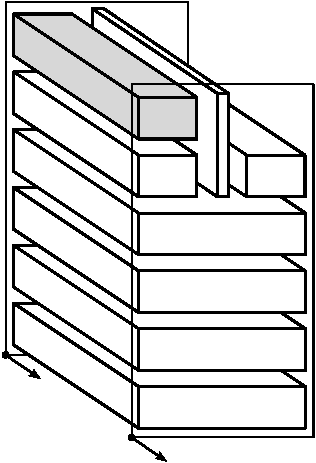
\includegraphics[scale=0.5]{ch3/img/PA_map_emulation.pdf}
\end{marginfigure}

\myparagraph{Optimization}
In parallel with the previous searching method, an emulation of the real field is implemented. The emulation tries to understand the position of the source as a solution of an optimization problem, using previous solution as a guess that is adapted through time. The optimization problem is:
\begin{equation}
\begin{array}{ll}
\underset{\mathbf{p}_T}{\mathrm{arg~min}} & \boldsymbol{\delta} \\
\mathrm{subject~to} & 	\left\{ \begin{array}{l}
							\boldsymbol{\delta} = \braces{\hfield(\hexastate,\mathbf{p}_T, \mathbf{m}) - \hat{\hfield}}^2 \\
							\braces{\hexastate - \mathbf{p}_T}^2  \leq  {\radiodist_{\mathrm{max}}}
						\end{array} \right. \\ 
\end{array}
\end{equation}
The optimization problem is solved numerically, guessing as initial point the solution at the previous step. The unilateral constraint is transformed in a barrier function.

The solution of the optimization routine is saved in a persistent memory, as a vector:
\[ \mathbf{P} = [ \mathbf{p}_{T,k} \,:\, k=1..N ] \]

\myparagraph{Estimation}
At this point, with could notice a lot of fluctuation in the solution, due to the noise in measurement, that is why we decided to treat the solution as a stochastic process. The solution are parsed in a \emph{parzen window estimator}, a non--parametric estimator, that consider a kernel function $\kernel$ with volume $V(h)$:
\begin{itemize}
\item $h$ identifies a kernel geometric characteristic
\item the kernel is normal: 
\[ \int\limits_{\mathbb{R}^n} \dfrac{\kernel}{V(h)}d\mathbf{p} = 1 \]
\item $\gamma(\cdot)$ has maximum in the origin
\item $\gamma(\cdot)$ is continuous
\item $\gamma(\pmb{\mu}\leftarrow\infty)\leftarrow 0$
\end{itemize}
the approximation of the distribution of the solution of the optimization step is in the form:
\begin{equation}
\hat{p}(\mathbf{p}) = \dfrac{1}{N}\sum\limits_{k=1}^{N} \dfrac{\gamma(\mathbf{p}-\mathbf{p}_k,h)}{V(h)}
\end{equation}
We have chosen as kernel a Gaussian function: 
\[ \int\limits_{-\infty}^{\infty} \dfrac{1}{\sqrt{2\pi} h} e^{-\dfrac{z^2}{2 h^2}} dz = 1 \]
Such an estimator has the following drawbacks:
\begin{itemize}
\item with the exact knowledge of the distribution that we are trying to estimate, the expectation of the estimation shows us that such an estimation is a blurred version of the real one: \[{E\{\hat{p}(\mathbf{p})\} = p(\mathbf{p}) * \dfrac{1}{h} \gamma(\mathbf{p},h)}\]
\item the estimation may suffer bias problem for samples $N<\infty$, that means \[{E\{\hat{p}(\mathbf{p})\}=E\{{p}(\mathbf{p})\} + \Delta}\]
\end{itemize}

The final concept of the estimator is to identify the position inside a certain circle of confidence. When the drone is in such a confidence area, it release the dart to signal the position to the rescue.

	\chapter{Simulations}
\minitoc
\thispagestyle{plain}

In this chapter we will see the implementation of part of the system using Matlab/Simulink platform. Some results are shown. Implementation takes into account the presence of noise in ARTVA receiver and consider a good estimation for the position and attitude of the system. To make simulation faster, we used \texttt{C--compiled} functions to perform heavier computational tasks\marginnote{The complete project is available on--line as a public Github repository. Please refer to the project for the actual source code of the single blocks.}. 

\section{Implementations}

\subsection{Dynamic model implementation}

The dynamic of the model is implemented with an \texttt{S-Function}, while the control is derived from the linearization of the model and thus inserted as gain in the model loop. The system has a free $\vrz$ attitude, while position is controlled through the use of an integrated velocity vector.
\begin{figure*}[h] \centering
\begin{tikzpicture}[auto,node distance=10mm and 7mm, >=latex']

	\node [block, fill=gray!40] (hexamodel) {Hexacopter Model};
	\fromworkspace{parameter}{\scriptsize{Parameters}}{at=(hexamodel),xshift=-50,yshift=30}
	\node [sum, left=of hexamodel] (sumA) {$+$};
	\node [block, left=of sumA] (force) {$F_i = \dfrac{mg}{6}$};
	
	\node [ellipse, draw, minimum width=1.3cm, above=of force] {\scriptsize{Time}};
	\node [block,below=of hexamodel] (controller) {LQR Controller};
	\node [block, right=of controller] (integrator) {$\dfrac{1}{s}$};
	\fromworkspace{zattitude}{\scriptsize{$\hat{\mathbf{z}}$ attitude}}{at=(controller),yshift=-30,xshift=-50}
	\node [sum, right=of integrator] (sumB) {$+$};
	\node [block, right=of sumB, text width=2cm,align=center] (searching) {Searching Algorithm};
	\node [block, below=of searching, text width=2cm,align=center] (obstacle) {Obstacle Avoiding};
	\coordinate[at=(hexamodel),xshift=220] (intersection);
	\toworkspace{results}{$\mathbf{x}$}{right=of intersection};

	\draw [->] (force) -- (sumA);
	\draw [->] (sumA) -- (hexamodel);
	\draw [->] (hexamodel) -- (results_in);
	\draw [->] (searching) -- (sumB);
	\draw [->] (sumB) -- (integrator);
	\draw [->] (integrator) -- (controller);

	\draw [->] (controller) -| (sumA);
	\draw [->] (zattitude_out) -| (controller);
	\draw [->] (parameter_out) -| (hexamodel);
	\draw [->] (obstacle) -| (sumB);
	\draw [->] (intersection) |- (searching);
	\draw [->] (intersection) |- (obstacle);

\end{tikzpicture}
\caption{System complete model}
\end{figure*}
\begin{figure*}[h] \centering
\begin{tikzpicture}[auto,node distance=10mm and 7mm, >=latex]
	\inputpin{stato}{$\mathbf{x}$}{}
	\draw [at=(stato), xshift=50, fill=black] ++(0,0) node(muxin){} -- ++(0,2cm) -- ++(1mm,0) -- node[pos=0.2](posizione){} node[pos=0.4](velocita){} node[pos=0.6](angolo){} node[pos=0.8](velrotazione){} ++(0,-4cm) -- ++(-1mm,0) -- cycle;
	\node [sum, at=(posizione), xshift=50] (sumA) {$+$};
	\node [sum, at=(angolo), xshift=100] (sumB) {$+$};
	\draw [at=(stato), xshift=200+1mm, fill=black] ++(0,0) node(muxout){} -- ++(0,2cm) -- ++(-1mm,0) -- node[pos=0.2](posizioneB){} node[pos=0.4](velocitaB){} node[pos=0.6](angoloB){} node[pos=0.8](velrotazioneB){} ++(0,-4cm) -- ++(1mm,0) -- cycle;
	\node [gain,at=(stato.west), xshift=255, regular polygon rotate=-90] (gain) {$K$};
	\outputpin{controllo}{$\mathbf{u}$}{at=(stato.west), xshift=315};

	\inputpin{refer}{$\mathbf{x}_f$}{at=(stato.center), yshift=-80}
	\inputpin{attitz}{$\psi_f$}{at=(stato.center), yshift=-110}

	\draw [->] (stato_out) -- (muxin.center);
	\draw [->] (posizione.west) -- node[text width=1.5cm,align=left,pos=0.60]{\scriptsize{Position}} (sumA.west);
	\draw [->] (sumA.east) -- (posizioneB.west);
	\draw [->] (velocita.west) -- node[text width=1.5cm,align=left,pos=0.175]{\scriptsize{Velocity}} (velocitaB.west);
	\draw [->] (angolo.west) -- node[text width=1.5cm,align=left,pos=0.275]{\scriptsize{Attitude}} (sumB.west);
	\draw [->] (sumB.east) -- (angoloB.west);
	\draw [->] (velrotazione.west) -- node[text width=1.5cm,align=left,pos=0.175]{\scriptsize{Ang.ratio}} (velrotazioneB.west);
	\draw [->] (muxout.center) -- (gain);
	\draw [->] (gain) -- (controllo_in);

	\draw [->,draw=white,line width=2] (refer_out) -| (sumA.south);
	\draw [->,draw=white,line width=2] (attitz_out) -| (sumB.south);
	\draw [->] (refer_out) -| node[right,at end]{$-$} (sumA.south);
	\draw [->] (attitz_out) -| node[right,at end]{$-$} (sumB.south);

\end{tikzpicture}
\caption{Tracking problem}
\end{figure*}
\FloatBarrier

\subsection{Receiver Model}

The receiver implements a mean sampler to reduce white Gaussian noise. The model of the receiver contains the equations of the H--field at which noise proportional to signal intensity on each antenna. The idea is to get \num{40}\si{\decibel} of signal to noise ratio, that is quite optimistic, but it is also the value declared from some manufacturer. Also algorithm may work with lower receiver SNR.
\begin{figure*}[h] \centering
\begin{tikzpicture}[auto,node distance=10mm and 10mm, >=latex]
	
	\inputpin{stato}{$\mathbf{x}$}{}
	\node [block, right=of stato_out,fill=gray!40] (Hfield) {$\mathbf{H}\left( \mathbf{x}, \mathbf{p}_T, \hat{\mathbf{m}} \right)$};
	\fromworkspace{mvector}{\scriptsize{Magnetic Dipole $\hat{\mathbf{m}}$}}{at=(Hfield),xshift=-60,yshift=30,text width=2.7cm}
	\fromworkspace{tpos}{\scriptsize{Transmitter position $\mathbf{p}_T$}}{at=(Hfield),xshift=-60,yshift=50,text width=2.7cm}

	\coordinate [right=of Hfield] (intersection);
	\node [block, below=of intersection,text width=1cm, align=center] (absolute) {$|\mathbf{H}|$};
	\node [sum, below=of absolute] (prod) {$\times$};
	\node [block, left=of prod] (noise) {$\mathcal{N}(\mathbf{0},\Sigma)$};
	\node [gain, right=of prod, regular polygon rotate=-90, text width=0.3cm] (gain) {\scriptsize{SNR}};
	\node [sum, at=(intersection), xshift=100] (somma) {$+$};
	\outputpin{hvalue}{$\mathbf{H}$}{right=of somma}

	\draw[->] (stato_out) -- (Hfield);
	\draw[->] (Hfield) -- (somma);
	\draw[->] (somma) -- (hvalue_in);
	\draw[->] (intersection) -- (absolute);
	\draw[->] (absolute) -- (prod);
	\draw[->] (noise) -- (prod);
	\draw[->] (prod) -- (gain);
	\draw[->] (gain) -| (somma);
	\draw[->] (mvector_out) -| (Hfield);
	\draw[->] (tpos_out) -| (Hfield);

\end{tikzpicture}
\caption{Receiver implementation}
\end{figure*}
\FloatBarrier

\subsection{Obstacle avoidance}

In the obstacle avoidance block we find a model of the receivers, written as a \texttt{mex--function}, and than the quite simple algorithm that allow us to avoid the obstacle generating a velocity vector orthogonal to the obstacle plane. This velocity vector is added to the searching input. This behavior is typical of the grounded paradigm.
\begin{figure*}[h] \centering
\begin{tikzpicture}[auto,node distance=10mm and 7mm, >=latex]
	\inputpin{stato}{$\mathbf{x}$}{}
	\coordinate [right=of stato_out] (intersectionA);
	\node [block, right=of intersectionA,fill=gray!40] (range_finder) {Range Finder Model ${d_i}$};
	\fromworkspace{punti}{\scriptsize{${\Psi = [\mathbf{x}_i:i=1..M]}$}}{at=(range_finder),xshift=-60,yshift=30,text width=2cm}
	\fromworkspace{parametri}{\scriptsize{$[h,\,\rho]$}}{at=(range_finder),xshift=-60,yshift=50,text width=2cm}
	\node [block, below=of range_finder] (rotmat) {${\mathcal{R}^T(\phi,\theta,\psi)}$};
	\node [block, right=of range_finder] (velocita) {${\mathbf{v}_b = \sum\limits_{i=1}^{6} v(d_i) \hat{\mathbf{u}}_i}$};
	\node [sum, right=of velocita] (prod) {$\times$};
	\outputpin{velout}{$\mathbf{v}$}{right=of prod}
	\fromworkspace{paramV}{\scriptsize{$[p_1,\,p_2,\,p_3]$}}{at=(velocita),xshift=-45,yshift=30}

	\draw [->] (stato_out) -- (range_finder);
	\draw [->] (range_finder) -- (velocita);
	\draw [->] (velocita) -- (prod);
	\draw [->] (prod) -- (velout_in);
	\draw [->] (intersectionA) |- (rotmat);
	\draw [->] (rotmat) -| (prod);
	\draw [->] (punti_out) -| (range_finder);
	\draw [->] (parametri_out) -| (range_finder);
	\draw [->] (paramV_out) -| (velocita);

\end{tikzpicture}

\caption{Obstacle avoidance sub--block}
\end{figure*}
\FloatBarrier

\subsection{Searching algorithm}

The receiver output feeds directly the two component of the source searching algorithm. The field information is transformed in an intensity and in a direction value to get an exploration direction. Measured field is used to perform the emulation, as an optimization problem. It was quite tricky to call the optimizer from Simulink, but possible using the \texttt{caller extrinsic} directive, alongside with an external evaluation from the Matlab engine, using \texttt{feval}. To speed up the process, residuals and barrier function results are evaluated using a \texttt{mex--function}. The parzen window estimation is performed offline, only as qualitative expression of the quality of the algorithm. The system shows some problem due to the symmetry of the transmitting field.
\begin{figure*}[h] \centering
\begin{tikzpicture}[auto,node distance=10mm and 7mm, >=latex]
	\inputpin{stato}{$\mathbf{x}$}{}
	\coordinate [right=of stato_out] (intersectionA);
	\node [block, right=of intersectionA] (Hfield) {$\mathbf{H}$ sensor};
	\fromworkspace{mvector}{\scriptsize{Magnetic Dipole $\hat{\mathbf{m}}$}}{at=(Hfield),xshift=-60,yshift=30,text width=2.7cm}
	\fromworkspace{tpos}{\scriptsize{Transmitter position $\mathbf{p}_T$}}{at=(Hfield),xshift=-60,yshift=50,text width=2.7cm}
	\coordinate [right=of Hfield] (intersectionB);
	\node [block, right=of intersectionB] (direction){$\begin{array}{l} |\mathbf{H}| \\ \cos(\theta) \\ \sin(\theta) \end{array}$};
	\node [block, right=of direction] (filtering) {$\dfrac{\alpha_1 s + 1}{\beta_1 s^2 + \beta_2 s +1}$};
	\node [block,right=of filtering,text width=2cm,align=center] (velocity) {Exploration direction};
	\outputpin{velout}{$\mathbf{v}$}{right=of velocity}
	\node [block,below=of filtering,fill=gray!40,text width=3cm,align=center, minimum height=2cm] (emulation) {Emulation ${(\mathbf{H} - \hat{\mathbf{H}})^2 = \mathbf{0}}$};
	\coordinate [at=(emulation.east), yshift=15] (emulation_out1);
	\coordinate [at=(emulation.east), yshift=-15] (emulation_out2);
	\coordinate [at=(emulation.west), yshift=15] (emulation_in1);
	\coordinate [at=(emulation.west), yshift=-15] (emulation_in2);

	\toworkspace{posopt}{Optimized $\mathbf{p}_T$}{right=of emulation_out1}
	\toworkspace{mopt}{Optimized $\hat{\mathbf{m}}$}{right=of emulation_out2}
	\fromworkspace{paramV}{\scriptsize{Parameters}}{at=(velocity),xshift=-45,yshift=30}

	\draw [->] (mvector_out) -| (Hfield);
	\draw [->] (tpos_out) -| (Hfield);
	\draw [->] (stato_out) -- (Hfield);
	\draw [->] (Hfield) -- (direction);
	\draw [->] (direction) -- (filtering);
	\draw [->] (filtering) -- (velocity);
	\draw [->] (velocity) -- (velout_in);
	\draw [->] (intersectionA) |- (emulation_in2);
	\draw [->] (intersectionB) |- (emulation_in1);
	\draw [->] (emulation_out1) -- (posopt_in);
	\draw [->] (emulation_out2) -- (mopt_in);
	\draw [->] (paramV_out) -| (velocity);
\end{tikzpicture}

\caption{Searching algorithm sub--block}
\end{figure*}
\FloatBarrier

\section{Results}

\TODO{Immagini risultato}
	\chapter{Conclusions}
\minitoc

We have explored many different topics through this work. It is not easy to find a common line to derive conclusion about the future of such a kind of project. 

\section{The ARTVA and the searching field}

The digital ARTVA we have build is not ready to be used on a drone. The SNR is too high, and the receiving distance too small. Also the use of a complete analogical preamplifier should be avoided due to thermal derive.

What should be concluded from this analysis is:
\begin{itemize}
\item it is possible to build an ARTVA receiver relying only on normative data
\item the performance of a complete analogical preamplifier circuit tells us that other architecture should be preferred
\end{itemize}

It could be a good starting point remove the pre--amplification section, and \textbf{insert an high speed sampling device}, like an FPAA or an FPGA. Those device grant a sampling rate that is extremely higher with respect to a micro--controller, and antenna input could be directly sampled to implement more intense filtering routines. The use of such devices increases also the thermal reliability of the receiver, through the elimination of analog passive components in the filter. 

The receiver low performance may also be taken back to the low quality of the antenna. \textbf{Building a ferrite loop antenna} require a profound radio amateur experience and some specific instrumentation to characterize the winded loop. It is almost impossible to build two equal antenna, that is why a direct AD conversion is highly advised, and a dynamical calibration may be implemented via software.

The receiver is not the only critical part, some word must be spent about the complexity of the \textbf{searching H--field} and the transmission protocol. Even if based upon some strong advantages due to little interference induced by external environment, the protocol is defined in such a way that is almost impossible to perform a reliable searching routine. The use of one frequency, with such long $\lunghezzaonda$ put us in the difficult situation of searching in near field condition. As we have already seen, the field lines creates a very difficult shape to be interpreted.

The protocol has a \textbf{extremely variable duty cycle}, that is not a problem for a human rescuers, but could introduce issues in our algorithms, that make them unreliable.

Some simpler aspects of a construction of transmitting device are also locked by the normative, like battery. The use of commercial batteries is forced, while some other form of accumulator, with higher energy density, may be used. More energy could bring to the use of \textbf{different frequency transmitted}, to perform searches in near and far field, and send some more data.

The last element that should be taken into account is the impossibility to find two or more buried that are close to each other. The \textbf{signal overlapping problem} do not allow us to understand and sometime even receive the weaker signal. At this moment the only solution seems to be an estrangement from the buried found, to try to receive other beacons signal.

\textit{What is suggested in literature is a revision of the searching protocol and normative, to get a new one more conform to the technology evolution and to get a signal that is defined in such a way that could be used to perform an automatic searching routine.}

\section{The drone and its avionic}

The system presented is not ready to be implemented as a complete project. Many study should be performed to adapt the avionic to the duty cycle problem, and a better device, with higher SNR ratio must be implemented. 

From the mechanical point  of view, the use of an hexa--copter is due to the need of a very strong thrust vector to be robust with respect to wind gust, but a system to identify a continuous interference like constant wind that drone may encounter. 

The \textbf{perception--action map} fit completely the avionic problem, and its definition makes really easy to implement other high level routines, to expand searching capabilities and scope of use of our drone. With respect to literature, our map implement a tri--dimensional expansion in which two different behavior are accessed through an algorithm, the radar detection routine. This intuition is almost new to the theory, and is something that allow us to expand the embodiment of the agent.

Searching is performed in two step: an \textbf{exploration} and a \textbf{source searching and emulation}. Exploration gives the drone the ability to cover the avalanche front in search for a signal. When a signal is received and identified with the \textbf{radar detection} algorithm, the drone enter in fine searching method. The exploration tries to reach the maximum signal strength, avoiding impasse due to the field geometry, no matter what orientation magnetic dipole vector has.

The \textbf{emulation routine}, that runs in parallel, and represent the action part of the searching routine, tries to optimize numerically the equation of the field with respect to drone location to understand the position of the source. Simulation showed us that this formulation is not ready to be used on the field, even if it is a good starting point for a built from scratch searching algorithm. The symmetry of the field generates more than one single solution for the system of equations, and noise influences the results. More information should be provided to the optimization routine, in particular from the exploration: the exploring direction information may reduce the area in which source could be, from a sphere to an hemisphere, reducing optimization error. Also knowledge about avalanche plane could help us to limit the position of the source under the avalanche. Restriction to solution space increases our chances to find the global minimum of the optimization that refers to our buried position.

For what concerns \textbf{obstacle avoidance}, the algorithm presented generates a simple run away speed from obstacle. This means that we have no symbolical knowledge of the surroundings, decision derived from the fact that our computational resources are limited and mainly focused on the searching of the buried position. Parameter of the avoidance velocity should be chosen wisely, with respect to searching velocity.

The perception--action map may take advantages from different future sensor--fusion insertion, like video feed. Implementation of higher complexity will require an external element, like ground station with higher computational power, and an employment of a wireless communication bus, to exchange mission information. Also, a speech--to--text over radio could be used as a fast way to allow communication between rescuers and drone.

\emph{This work poses some foundation for the develop of an agent that is able to find a buried victim on the avalanche. The performance of the agent can not be completely related to the definition of its searching algorithm, but also due to the complexity of the ARTVA protocol. Taken this problem apart, perception action map showed us how it is possible to implement a complete avionic, and get an autonomous drone, prone to further modification and expansions.}

\backmatter
	\renewcommand{\headrulewidth}{0pt}
	\thispagestyle{empty}
	\listofsymbolspages
	\setlength{\parskip}{5pt}
	\bibliographyinsert
	\setlength{\parskip}{0pt}
	%\listoffigures
	%\index ?? we will see...

\end{document}